\AtBeginDocument{%
  \providecommand\BibTeX{{%
    Bib\TeX}}}

\documentclass[acmsmall,screen,review=false]{acmart}

%%%%% THe following four lines remove the copyright notice on the first page.
%%%% \setcopyright{none}
%%%% \settopmatter{printacmref=false} % Removes citation information below abstract
%%%% \renewcommand\footnotetextcopyrightpermission[1]{} % removes footnote with conference information in first column
%%%% \pagestyle{plain}

\usepackage{booktabs}
\usepackage{amsthm}
\usepackage{amsmath}
\usepackage{qcircuit}
\usepackage{multirow}
\usepackage{graphicx}
\usepackage{wrapfig}
\usepackage{soul}
\setstcolor{red}
\usepackage{color, xcolor}

\usepackage{tikz}
\usetikzlibrary{shapes.geometric, arrows}
\tikzstyle{startstop} = [rectangle, rounded corners, minimum width=2.4cm,
           minimum height=1cm,text centered, draw=black, fill=red!30]
\tikzstyle{bottomlayer} = [rectangle, rounded corners, minimum width=2.4cm,
           minimum height=1cm,text centered, draw=black, fill=green!30]
\tikzstyle{arrow} = [thick,->,>=stealth]

\def\ket#1{|#1\rangle}
\def\bra#1{\langle#1|}
\def\inner#1#2{\langle{#1}|{#2}\rangle}
\def\outer#1#2{\ket{#1}\bra{#2}}
\def\eigenvalues#1{\mbox{\sf Eigenvalues}(#1)}

\def\diag#1{\mbox{\sf Diag}{(#1)}}
\def\diagtwo#1#2{\diag{#1,#2}}

\def\C#1{\mbox{\sf C}{(#1)}}
\def\CC#1{\mbox{\sf CC}{(#1)}}

\def\oU{\overline{U}}
\def\oV{\overline{V}}
\def\oS{\overline{S}}

\def\SS{{\mathcal{S}}}

\newtheorem{theorem}{Theorem}[section]
\newtheorem{lemma}[theorem]{Lemma}
\newtheorem{example}[theorem]{Example}

\newtheorem{thm}{Theorem}
\newenvironment{thmbis}[1]
  {\renewcommand{\thethm}{\ref{#1}}%
   \addtocounter{thm}{-1}%
   \begin{thm}}
  {\end{thm}}

\newtheorem{lem}{Lemma}
\newenvironment{lembis}[1]
  {\renewcommand{\thelem}{\ref{#1}}%
   \addtocounter{thm}{-1}%
   \begin{lem}}
  {\end{lem}}

\citestyle{acmauthoryear}

% \newtheorem{example}{Example}


% \author{ANONYMOUS AUTHOR(S)}

\begin{document}

%%
%% The "title" command has an optional parameter,
%% allowing the author to define a "short title" to be used in page headers.
\title{Toffoli Requires Six Quantum Neighbor Gates}

%%
%% The "author" command and its associated commands are used to define
%% the authors and their affiliations.
%% Of note is the shared affiliation of the first two authors, and the
%% "authornote" and "authornotemark" commands
%% used to denote shared contribution to the research.
\author{Keli Huang}
\affiliation{
\institution{University of California, Los Angeles}
\country{USA}}
\email{kelihuang@cs.ucla.edu}

\author{Jens Palsberg}
\affiliation{
\institution{University of California, Los Angeles}
\country{USA}}
\email{palsberg@ucla.edu}

\renewcommand{\shorttitle}{Toffoli Requires Six Quantum Neighbor Gates}
\renewcommand{\shortauthors}{Keli Huang and Jens Palsberg}

\begin{abstract}
Toffoli gates are key building blocks in quantum programs, and on
most current quantum computers, they must be implemented with smaller gates.
Such an implementation requires five 2-qubit gates if we assume that each gate can operate on any two qubits.
However, many current quantum computers have only 2-qubit gates that operate on neighboring qubits; we call them neighbor gates.
How many neighbor gates are required to implement a Toffoli gate?
In this paper, we show that six neighbor gates are necessary and sufficient,
and we generalize to a characterization of all 3-qubit diagonal gates.
\end{abstract}

\begin{CCSXML}
<ccs2012>
<concept>
<concept_id>10010520.10010521.10010542.10010550</concept_id>
<concept_desc>Computer systems organization~Quantum computing</concept_desc>
<concept_significance>500</concept_significance>
</concept>
<concept>
<concept_id>10011007.10011006.10011041</concept_id>
<concept_desc>Software and its engineering~Compilers</concept_desc>
<concept_significance>500</concept_significance>
</concept>
</ccs2012>
\end{CCSXML}

\ccsdesc[500]{Computer systems organization~Quantum computing}
\ccsdesc[500]{Software and its engineering~Compilers}


%
%% The code below is generated by the tool at http://dl.acm.org/ccs.cfm.
%% Please copy and paste the code instead of the example below.

\keywords{quantum computing, compilers, code size}

\maketitle

%%
%% The abstract is a short summary of the work to be presented in the
%% article.

% \section*{TODO LIST}
 
% \begin{enumerate}
%    \item Give a more intuitive understanding of the main result. 
    
%    \textcolor{blue}{Done.  We have added an explanation to Section 1.}

%    \item Section 4 specifies seven different sets of gates. The sets are defined by eigenvalues of the gates satisfying certain relations. The relations came seemingly out of nowhere, with no intuition provided for what these sets are or where the relations came from. Four of these sets/relations appear to have come from prior work. But even so, the old sets could've been explained, and certainly the new sets need some discussion. 

%    \textcolor{blue}{Done.  We have added an explanation to Section 4.} 

%    \item The paper provides zero intuition for the proof, neither in the first 10 pages, nor in the appendix where it is given in full. This makes it hard to understand the paper. Explain the techniques used in the proof.

%    \textcolor{blue}{Done.  We have added an explanation to Section 1, and we have added a new section that gives the most important part of the proof.}

%    \item Explain the technical novelty over the existing work. It is hard to understand the novelty over the existing work.

%    \textcolor{blue}{Done.  We have added an explanation to Section 1.}

%    \item A weakness of this paper is that it assumes that the Toffoli is acting on "adjacent" qubits (i.e. on a connected graph of size 3), which seems a bit strong to me, as in general to implement a Toffoli, you would then have to first swap the three qubits into neighboring positions. 

%    \textcolor{blue}{Done.  We have added an explanation to Section 3.}

%    \item change the format to TQC format.

%    \textcolor{blue}{Done. They use the same ACM format as POPL, PLDI.}

% \end{enumerate}

\section{Introduction}

% Toffoli gates are key building blocks in quantum programs,

\paragraph{Background.}
Researchers are designing quantum algorithms that, in some cases, have an exponential advantage over classical algorithms.
They describe their algorithms in the form of quantum circuits that use quantum gates.
In a recent trend, many of their papers
\cite{berry2019qubitization, 
su2021fault, 
lee2021even, 
goings2022reliably, 
rubin2024quantum, 
berry2024analyzing}
express an algorithm's execution time in terms of the number of Toffoli gates.
They do that because they anticipate error-corrected quantum computers on which
the execution of Toffoli gates will be a bottleneck.
Thus, they use Toffoli gates as building blocks that must be compiled to hardware gates.

% on most current quantum computers,
% they must be implemented using smaller gates.
% Such implementation requires five 2-qubit gates, if we assume that
% all qubits are connected.

Toffoli gates are 3-qubit gates and on most current quantum computers,
they must be implemented with smaller gates.
Thus, the implementation of a Toffoli gate on a given quantum computer has a direct impact on the execution time of quantum algorithms.
For such an implementation, five 2-qubit gates are necessary and sufficient, as shown by
\cite{YuDuanYing13,YuYing15,palsberg2024optimal}, assuming that a 2-qubit gate can operate on any two qubits.  
In our terminology, such an implementation uses {\em unrestricted} gates.

Current quantum computers rarely support that a 2-qubit gate can operate on any two qubits.
For example, IBM Condor (1,121 qubits) and IBM Osprey (433 qubits) support that
a 2-qubit gate operates only on some pairs of qubits.
In particular, for any three qubits, they support 2-qubit gates on at most two of the three possible pairs of qubits.
They do that because supporting a 2-qubit gate is easier when the two qubits are neighbors on the chip.
In our terminology, current quantum computers tend to support {\em neighbor} gates.

In this paper, we focus on the question of how many 2-qubit neighbor gates
are required to implement a Toffoli gate and, more generally, any 3-qubit diagonal gate.

  
\paragraph{Question: Five or Six?}

% This raises the question of how many 2-qubit neighbor gates
% are required to implement a Toffoli gate.
% Related work on CNOT: 1) CNOT-cost of Toffoli, 2) ASPLOS 2021.
% We want hardware-independent results.

% Duckering et al.\ 

% We can implement a Toffoli gate using eight $\C{X}$ neighbor gates and some 1-qubit gates, as shown by
% \cite{duckering2021orchestrated}.
We can implement a Toffoli gate both using five unrestricted gates \cite{YuDuanYing13}, and using six neighbor gates, as we show in Section~\ref{sec:programming-with-neighbor-gates}.
Here we arrive at our central question: {\em five or six?}
Specifically, can we improve the implementation of a Toffoli gate from using five unrestricted gates to using five neighbor gates?
Or, are we forced to use a sixth neighbor gate?

\paragraph{Our Results.}

% In this paper, we show that six neighbor gates are necessary and sufficient,
% and we generalize this result to a characterization of all diagonal gates.
% A special case: if \CC{U}, where det(U) = 1, then four is enough.
We show that six neighbor gates are necessary and sufficient to implement a Toffoli gate.
We also generalize this to a characterization of
the number of neighbor gates (Theorem~\ref{thm:optimal-neighbor-implementation-of-3-qubit-diagonal-gates}) and
the number of unrestricted gates (Theorem~\ref{thm:optimal-implementation-of-3-qubit-diagonal-gates})  
that \textcolor{black}{are sufficient} to implement 3-qubit diagonal gates. 
\textcolor{black}{In Corollary~\ref{cor:least-upper-bounds}, we prove that these upper bounds are indeed least upper bounds. }

\paragraph{Our Proof Technique.}
\textcolor{black}{Figure~\ref{fig:proof-structure} shows our proof structure.} 
%
\begin{figure}[ht]
    \centering
    \begin{center}
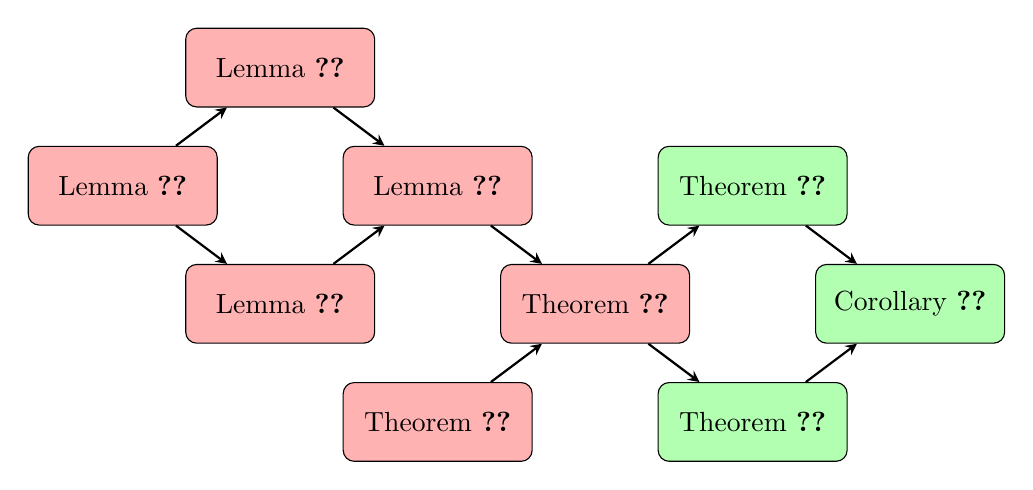
\begin{tikzpicture}[node distance=2cm]
\node (lemma1) [startstop]
   {Lemma~\ref{1keylemma}};
\node (lemma2) [startstop, right of=lemma1, yshift=1.5cm]
   {Lemma~\ref{firstlemma}};
\node (lemma3) [startstop, right of=lemma1, yshift=-1.5cm]
   {Lemma~\ref{secondlemma}};
\node (lemma4) [startstop, right of=lemma3, yshift=1.5cm]
   {Lemma~\ref{lemma:diag-5-to-4}};
\node (theorem6-1) [startstop, right of=lemma3, yshift=-1.5cm]
   {Theorem~\ref{lem:s4-s5-if-and-only-if-product-of-four-neighbor-gates}};
\node (theorem6-2) [startstop, right of=theorem6-1, yshift=1.5cm]
   {Theorem~\ref{nearest neighbor4}};
\node (theorem7-1) [bottomlayer, right of=theorem6-2, yshift=1.5cm]
   {Theorem~\ref{thm:optimal-neighbor-implementation-of-3-qubit-diagonal-gates}};
\node (theorem7-2) [bottomlayer, right of=theorem6-2, yshift=-1.5cm]
   {Theorem~\ref{thm:optimal-implementation-of-3-qubit-diagonal-gates}};
\node (corollary) [bottomlayer, right of=theorem7-2, yshift=1.5cm]
   {Corollary~\ref{cor:least-upper-bounds}};
\draw [arrow] (lemma1) -- (lemma2);
\draw [arrow] (lemma1) -- (lemma3);
\draw [arrow] (lemma2) -- (lemma4);
\draw [arrow] (lemma3) -- (lemma4);
\draw [arrow] (lemma4) -- (theorem6-2);
\draw [arrow] (theorem6-1) -- (theorem6-2);
\draw [arrow] (theorem6-2) -- (theorem7-1);
\draw [arrow] (theorem6-2) -- (theorem7-2);
\draw [arrow] (theorem7-1) -- (corollary);
\draw [arrow] (theorem7-2) -- (corollary);
\end{tikzpicture}
\end{center}
    \caption{Proof structure.}
    \label{fig:proof-structure}
\end{figure}
The lower bound for implementations of a Toffoli gate is a corollary of Theorem~\ref{nearest neighbor4}, which is a novel equivalence between the expressive power of unrestricted gates and the expressive power of neighbor gates.
Specifically, Theorem~\ref{nearest neighbor4} says that three classes of quantum circuits implement the same 3-qubit diagonal gates;
those classes are
(1) four neighbor gates,
(2) five neighbor gates, and
(3) four unrestricted gates.
The most surprising aspect of Theorem~\ref{nearest neighbor4} is the implication $(2) \Rightarrow (1)$, which says that we can transform any circuit with five neighbor gates into an equivalent circuit with four neighbor gates.
This may seem like a magic trick: a gate disappeared!
We prove Theorem~\ref{nearest neighbor4} by proving the chain of implications $(1) \Rightarrow (2) \Rightarrow (3) \Rightarrow (1)$.

The proof of the implication $(2) \Rightarrow (3)$ is
the main technical innovation in this paper: we transform an implementation of a 3-qubit diagonal gate using five neighbor gates into an implementation using four unrestricted gates.  We devote Section~\ref{sec:from-five-neighbor-gates-to-four-unrestricted-gates} to proving one particular form of this result (Lemma~\ref{lemma:diag-5-to-4}), 
\textcolor{black}{which uses Lemmas~\ref{1keylemma}--\ref{secondlemma},}
and then we use it in Section~\ref{sec:toffoli-requires-six-neighbor-gates} in the proof of Theorem~\ref{nearest neighbor4} \textcolor{black}{which relies on Theorem~\ref{lem:s4-s5-if-and-only-if-product-of-four-neighbor-gates}}.
Our proofs in 
Section \ref{sec:from-five-neighbor-gates-to-four-unrestricted-gates} \textcolor{black}{and Section} \ref{sec:toffoli-requires-six-neighbor-gates} rely on a suite of known lemmas that we list in Appendix~\ref{sec:known-lemmas}.
In particular, we use Lemma~\ref{lemma6.4} (\cite[\textsc{Lemma} 6.4]{palsberg2024optimal}), which characterizes the 3-qubit quantum gates with two controls that can be implemented with four neighbor gates. 

A surprising corollary of Theorem~\ref{nearest neighbor4} is that
while {\em four} unrestricted gates and {\em four} neighbor gates have the {\em same} expressive power, 
{\em five} unrestricted gates have {\em strictly more} expressive power than {\em five} neighbor gates.
In particular, five unrestricted gates are sufficient to implement a Toffoli gate, while five neighbor gates are insufficient.
Another surprising finding is that, in some cases, the qubit layout affects the optimal number of neighbor gates (Theorem~\ref{lem:s4-s5-if-and-only-if-product-of-four-neighbor-gates}).

\paragraph{The Rest of the Paper.}
In Section~\ref{sec:quantum-concepts}, we recall key quantum concepts, and
in Section~\ref{sec:programming-with-neighbor-gates}, we show implementations of the Toffoli gate and two other gates.
In Section~\ref{sec:sets-of-3-qubit-diagonal-gates}, we define some sets of 3-qubit diagonal gates that we use to state our results, and
in Sections~\ref{sec:from-five-neighbor-gates-to-four-unrestricted-gates}--\ref{sec:full-characterization-of-3-qubit-diagonal-gates}, we state and prove our theorems, with the exception of some proofs that we relegated to the appendices. 
In Section~\ref{sec:our-example-circuits-are-optimal}, we use our theorems to show that our implementations in Section~\ref{sec:programming-with-neighbor-gates} are optimal, and
in Section~\ref{sec:related}, we discuss related work. 

\section{Quantum Concepts}
\label{sec:quantum-concepts}

% In this section, we introduce the quantum concepts that we use in the paper.

\paragraph{Qubits, Quantum States, and Quantum Gates.} A qubit is a two-dimensional unit vector of complex numbers. An $n$-qubit quantum state is a $2^n$-dimensional unit vector of complex numbers. We use lower-case letters $a$, $b$, $d$, $p$, $q$ to represent complex numbers. Furthermore, we use lowercase letters, enclosed in Dirac notation, as $\ket{x}$, $\ket{y}$, $\ket{z}$ to range over 1-qubit quantum states.

A quantum gate is a unitary matrix. A matrix $U$ is unitary if $U U^\dag = U^\dag U = I$, where $U^\dag$ is the conjugate transpose of $U$, and $I$ is the identity matrix.
%
We use uppercase letters, such as $U$, to range over quantum gates.
We will use the following gates. 
\[
\begin{array}{rclrclrcl}
S &=& \left[\!\!\begin{array}{cccc}
1 \!&\! 0 \!&\! 0 \!&\! 0 \\
0 \!&\! 0 \!&\! 1 \!&\! 0 \\
0 \!&\! 1 \!&\! 0 \!&\! 0 \\
0 \!&\! 0 \!&\! 0 \!&\! 1
\end{array}\!\!\right] 
&
X &=& \left[\!\!\begin{array}{cc}
0 & 1 \\
1 & 0
\end{array}\!\!\right]
\;\;\;\;\;
Z \;\;=\;\; \left[\!\!\begin{array}{cc} 
1 \!&\! 0 \\ 
0 \!&\! -1 \end{array}\!\!\right]
&
H &=& \frac{1}{\sqrt{2}} \left[\!\!\begin{array}{cc}
1 & 1 \\
1 & -1
\end{array}\!\!\right]
\\ \\
R_z(\alpha) &=& \left[\!\!\begin{array}{cc} 
e^{-i\frac{\alpha}{2}} \!&\! 0 \\ 
0 \!&\! e^{i\frac{\alpha}{2}} \end{array}\!\!\right]
\;\;
&
R_y(\theta) &=& \left[\!\!\begin{array}{cc} 
\cos(\theta/2) \!&\! -\sin(\theta/2) \\ 
\sin(\theta/2) \!&\! \cos(\theta/2) \end{array}\!\!\right]
&
P(\varphi) &=& \left[\!\!\begin{array}{cc}
1 & 0 \\
0 & e^{i\varphi}
\end{array}\!\!\right]
\end{array}
\]
Notice that $S$ is the 2-qubit swap gate, while the others are 1-qubit gates. Also, we have that $H Z H = X$, $H X H = Z$, and $H^\dag = H$.
%
We use Greek letters $\alpha$, $\beta$, $\gamma$, $\varphi$, and $\theta$ to stand for angles ranging from $0$ to $2\pi$.

We write an $n$-qubit diagonal gate with $2^n$ complex-number entries as $\diag{d_0, \  d_1, \ \dots \ , d_{2^{n}-1}}$, where $d_i$ is the $(i+1)^{th}$ element on the diagonal. 
%\textcolor{black}{We denote the 3-qubit diagonal gate $D = \diag{d_0, d_1, \ldots, d_7}$ for further discussion. }
% The diagonal gates only change the probability amplitude of each quantum state if each qubit is written in $\ket{0}$ and $\ket{1}$ computational basis states.

For an $n$-qubit gate $U$, we define 
its $(n+1)$-qubit zero-controlled gate as $\outer{0}{0} \otimes U + \outer{1}{1} \otimes I$,
which applies $U$ to the target qubits when the control qubit is $\ket{0}$ and applies the identity matrix if it is $\ket{1}$.
Also, we define 
its $(n+1)$-qubit one-controlled gate as $\C{U} = \outer{0}{0} \otimes I + \outer{1}{1} \otimes U$.
which applies $U$ to the target qubits when the control qubit is $\ket{1}$ and applies the identity matrix if it is $\ket{0}$.

\textcolor{black}{
We use $\eigenvalues{U}$ to denote the multiset of eigenvalues of the unitary matrix $U$, and we use $\sqcup$ to denote the multiset-union operator.}

\paragraph{Quantum Circuit Diagrams.} In a circuit diagram, each qubit has its own line, and we use the symbol $/$ to denote that a diagram represents multiple qubits in a single line. 
We display the $X$ gate as $\oplus$, and we display the $S$ gate as two $\times$'s connected by a line. 
In such a diagram, we have three special notations. 
%
We display a zero-controlled operation as $\circ$ and a one-controlled operation as $\bullet$, as shown in Figure~\ref{fig:zeroone}.
\begin{figure}[ht!]
\hspace*{1cm}
\begin{minipage}[t]{0.40\linewidth}
\hspace{1.0cm}
\Qcircuit @C=0.5em @R=0.45em {
& \qw & \ctrlo{2} &\qw 
&  &  &  &
& \qw & \multigate{2}{\C{U}}  & \qw &   &  & \qw & \ctrl{2} &\qw \\  
&             &           &    
&  &  &  &
& & &     & = &  &             &           & \\
&\qw / & \gate{U} &\qw 
&  &  &  &
& \qw / & \ghost{\C{U}}       & \qw &   &  &\qw / & \gate{U} &\qw\\
}
\caption{Circuits for controlled gates.}
\label{fig:zeroone}
\end{minipage}
\hspace*{0.5cm}
\begin{minipage}[t]{0.40\linewidth}
\hspace{0.7cm}
\Qcircuit @C=0.5em @R=0.45em {
& \qw & \multigate{2}{V} & \qw &   &  & \qw & \gate{} \qwx[2] & \qw &   &  & \qw & \ctrlo{2}      & \ctrl{2}       &\qw\\  
&  &  &  & =  &  & & &     & = &  &             &           &      &                \\
& \qw / & \ghost{V} & \qw &   &  & \qw / & \gate{V}       & \qw &   &  &\qw / & \gate{V_0}      & \gate{V_1}  &\qw\\
}
\caption{Zero-one-controlled circuits.}
\label{fig:boxcontrol}
\end{minipage}
\end{figure}

If there exist two $n$-qubit gates $V_0$ and $V_1$, such that an $(n+1)$-qubit gate $V$ can be written as $V = \outer{0}{0} \otimes V_0 + \outer{1}{1} \otimes V_1$, then, in a diagram, we use $\Box$ on a line to emphasize such a qubit, as shown in Figure~\ref{fig:boxcontrol}. We borrow this notation from \cite{shende2008cnot}. 

%If a 3-qubit gate $D$ has two zero-one-controlled qubits, then there exist four 1-qubit gates $D_{00}$, $D_{01}$, $D_{10}$, and $D_{11}$, such that $D = \outer{00}{00} \otimes D_{00} + \outer{01}{01} \otimes D_{01} + \outer{10}{10} \otimes D_{10} + \outer{11}{11} \otimes D_{11}$, as shown in Figure~\ref{fig:boxboxcontrol}. 
\textcolor{black}{For a 3-qubit diagonal gate $D = \diag{d_0, d_1, \dots, d_7}$, there exist four 1-qubit gates $D_{00} = \diag{d_0, d_1}$, $D_{01} = \diag{d_2, d_3}$, $D_{10} = \diag{d_4, d_5}$, and $D_{11} = \diag{d_6, d_7}$, such that $D = \outer{00}{00} \otimes D_{00} + \outer{01}{01} \otimes D_{01} + \outer{10}{10} \otimes D_{10} + \outer{11}{11} \otimes D_{11}$.  This enables us to think of $D$ in terms of two control qubits, and we display $D$ as shown in Figure~\ref{fig:boxboxcontrol}.}
\begin{figure}[ht!]
\begin{minipage}[t]{0.60\linewidth}
\hspace{1.4cm}
\Qcircuit @C=0.5em @R=1em {
& \qw & \gate{} \qwx[1] & \qw &   &  & \qw & \ctrlo{1} & \ctrlo{1} & \ctrl{1} & \ctrl{1} &\qw\\  
& \qw & \gate{} \qwx[1] & \qw & = &  & \qw & \ctrlo{1} & \ctrl{1} & \ctrlo{1} & \ctrl{1} &\qw\\
& \qw & \gate{D}        & \qw &   &  & \qw & \gate{D_{00}} & \gate{D_{01}} & \gate{D_{10}} & \gate{D_{11}}  & \qw \\
}
\caption{A gate with two zero-one-controlled qubits.}
\label{fig:boxboxcontrol}
\end{minipage}
\end{figure}

% Keli: I think we can delete this sentence. According to Lemma~\ref{commutez}, the gate $V$ commutes with the $Z$ % gates on the qubit where $\Box$ is located.

\paragraph{Applying a 2-qubit Gate to 3 Qubits.}
Because we focus on 3-qubit circuits, we use three uppercase letters $A$, $B$, $C$ to represent these three different qubits. 
An unrestricted 2-qubit gate can operate on any pair of qubits: $AB$, $BC$, and $AC$.
However, neighbor gates can operate on only two of the three pairs.  
Following \cite{palsberg2024optimal}, we define a 3-qubit gate $\overline{U}_{ij}$, where $ij \in \{ AB, \, BC, \, AC \, \}$, to represent that a 2-qubit gate $U$ is implemented on the qubits $i$ and $j$ in a 3-qubit circuit, with the third qubit remaining unchanged. In this notation, if $U$ is a 2-qubit unitary, then $U_{ij}$ operates on 2 qubits, while $\overline{U}_{ij}$ operates on 3 qubits. We define $\overline{U}_{ij}$ as follows.
\begin{eqnarray*}
\oU_{AB} &=& U \otimes I, \;\;\;\;\;\;\;\;
\oU_{BC} \;\;=\;\; I \otimes U, \;\;\;\;\;\;\;\;
\oU_{AC} \;\;=\;\; \oS_{BC}\ \oU_{AB}\ \oS_{BC}
\end{eqnarray*}
%
Notice the use of the swap gate $S$ in $\oS_{BC}$.
%
We have that $\oS_{AB}\ \oU_{AC}\ \oS_{AB} = \oU_{BC}$
\cite[\textsc{Lemma} A.12]{palsberg2024optimal}. 
Furthermore, we can easily check that
$\overline{S}_{BC}\,
\overline{S}_{AC}\,
\overline{U}_{AB}\, \overline{S}_{AC} \, \overline{S}_{BC} = 
\overline{U}_{BC}$. If we have qubit indices $ij \in \{BA, CB, CA\}$, then the qubit order must be reversed by sandwiching two swap gates. Thus, we write $\overline{U}_{ij}$ as $(\overline{S}_{ji}\ \overline{U}_{ji}\ \overline{S}_{ji})$ or $\overline{SUS}_{ji}$.
\textcolor{black}{
We write $\overline{UVW}_{ij}$ as an abbreviation for $\overline{U}_{ij}\, \overline{V}_{ij}\, \overline{W}_{ij}$.
}

% We define $R = \oS_{BC}\, \oS_{AC}$. 
% We can easily check that 
% R = \oS_{AB}\ \oS_{BC}$ and
% $R\ \oU_{AB}\ R^\dagger = \oU_{BC}$ and
% $R\ \oU_{AC}\ R^\dagger = \oS_{AB}\ \oU_{AB}\ \oS_{AB}$ and
% $R\ \oU_{BC}\ R^\dagger = \oS_{AC}\ \oU_{AC}\ \oS_{AC}$ and
% $R^\dagger\ \oU_{AC}\ R = \oS_{BC}\ \oU_{BC}\ \oS_{BC}$ and
% $R^\dagger\ \oU_{AB}\ R = \oS_{AC}\ \oU_{AC}\ \oS_{AC}$.

\paragraph{Sets of Gates.}
If $U,V$ are 3-qubit gates, and $\SS$ is a set of 3-qubit diagonal gates, then we define:
\begin{eqnarray*}
U\ \SS\ V &=& \{\ U\ D\ V \;|\; D \in \SS\ \}
\end{eqnarray*}


\section{Programming with Neighbor Gates}
\label{sec:programming-with-neighbor-gates}

In this section, we present five example circuits \textcolor{black}{that implement the Toffoli gate (Examples~\ref{sec:example-ccu-ab-bc}--\ref{sec:example-ccu-ac-bc}) and other diagonal gates (Examples~\ref{sec:example-ccw-ac-bc-detw-1}--\ref{sec:example-diag-on-ab-bc})}. They all have the optimal numbers of 2-qubit gates, as we will show in Section~\ref{sec:our-example-circuits-are-optimal}.

\paragraph{Qubit Layout.}
\label{sec:qubit-layout}

If we have three qubits $A$, $B$, and $C$, and only two of the pairs are neighbors, the qubit layout is one of the ones in Figure~\ref{fig:enter-label}.  We will study all three layouts.

\begin{figure}[ht!]
    \centering
    \begin{center}
    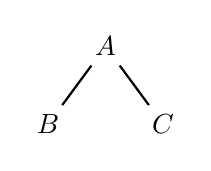
\begin{tikzpicture}[node distance=1.4cm]
    \node (top) {$A$};
    \node (left) [below left of=top, xshift=0.26cm] {$B$};
    \node (right) [below right of=top, xshift=-0.26cm] {$C$};

    % Edges
    \draw[thick] (top) -- (left);
    \draw[thick] (top) -- (right);
    % \draw (left) -- (right);
    \end{tikzpicture}
    %
    \hspace*{0.8cm}
    %
    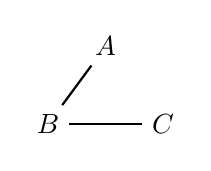
\begin{tikzpicture}[node distance=1.4cm]
    \node (top) {$A$};
    \node (left) [below left of=top, xshift=0.26cm] {$B$};
    \node (right) [below right of=top, xshift=-0.26cm] {$C$};

    % Edges
    \draw[thick] (top) -- (left);
    % \draw (top) -- (right);
    \draw[thick] (left) -- (right);
    \end{tikzpicture}
    %
    \hspace*{0.8cm}
    %
    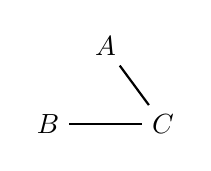
\begin{tikzpicture}[node distance=1.4cm]
    \node (top) {$A$};
    \node (left) [below left of=top, xshift=0.26cm] {$B$};
    \node (right) [below right of=top, xshift=-0.26cm] {$C$};

    % Edges
    % \draw (top) -- (left);
    \draw[thick] (top) -- (right);
    \draw[thick] (left) -- (right);
   \end{tikzpicture}
   \end{center}
    \caption{Three qubit layouts.}
    \label{fig:enter-label}
\end{figure}

\paragraph{The Toffoli Gate.}
\label{sec:the-toffoli-gate}

The Toffoli gate can be written $\CC{X}$, and it can be depicted as the left-hand-side of Circuit~(\ref{eq:quantum-compilation-scheme-for-ccx}).
Here, $A, B, C$ are qubits, and the idea is that if both $A$ and $B$ are 1, then the gate will flip $C$ by applying an $X$ gate.
The usual terminology is that $A, B$ are the control qubits, while $C$ is the target qubit.
The notation $\CC{X}$ signals that the gate has two control qubits and that we may apply an $X$ gate to the target qubit.
%
Below is an implementation of a Toffoli gate that uses five unrestricted gates, which is the optimal number of such gates.
Those gates are all conditional gates that each has a single control.  
%
\begin{eqnarray}
\Qcircuit @C=0.5em @R=1em {
\lstick{A} & \ctrl{1} & \qw & & & & & 
\ctrl{2} & \qw & \ctrl{1} & \qw & \ctrl{1} & \qw \\
\lstick{B} & \ctrl{1} & \qw  & & = & & & 
\qw & \ctrl{1} & \targ & \ctrl{1} & \targ & \qw \\
\lstick{C} & \targ & \qw  & & & & & 
\gate{\sqrt{X}} & \gate{\sqrt{X}} & \qw & \gate{\sqrt{X}^\dag} & \qw & \qw \\
}
\label{eq:quantum-compilation-scheme-for-ccx}
\end{eqnarray}
%
Notice that in Circuit~(\ref{eq:quantum-compilation-scheme-for-ccx}), the gates are applied to all possible qubit pairs $AC$, $BC$, and $AB$.

\paragraph{A Gate with Two Controls.}
We can generalize $\CC{X}$ to $\CC{U}$ where $U$ is a 1-qubit unitary, and we can implement it by a straightforward generalization of the scheme above.
%
\begin{eqnarray}
\Qcircuit @C=0.5em @R=1em {
\lstick{A} & \ctrl{1} & \qw & & & & & 
\ctrl{2} & \qw & \ctrl{1} & \qw & \ctrl{1} & \qw \\
\lstick{B} & \ctrl{1} & \qw  & & = & & & 
\qw & \ctrl{1} & \targ & \ctrl{1} & \targ & \qw \\
\lstick{C} & \gate{U} & \qw  & & & & & 
\gate{\sqrt{U}} & \gate{\sqrt{U}} & \qw & \gate{\sqrt{U}^\dag} & \qw & \qw \\
}
\label{eq:quantum-compilation-scheme-for-ccu-with-two-controls}
\end{eqnarray}

In Table~\ref{sec2_table}, we walk through the effect of Circuit~(\ref{eq:quantum-compilation-scheme-for-ccu-with-two-controls}) on $\ket{AB} \ket{C}$, and we see that 
the circuit implements $\CC{U}$ correctly: the final state is $\ket{AB}\ U\ket{C}$ if and only if $\ket{AB} = \ket{11}$, and $\ket{AB}\ \ket{C}$ otherwise.

\begin{table}[ht!]
\caption{The effect of the circuit in (\ref{eq:quantum-compilation-scheme-for-ccu-with-two-controls}) on $\ket{AB}\ \ket{C}$.}
\label{sec2_table}
\begin{center}
\begin{tabular}{ccccccc}
    % \toprule
    Input & ${\C{\sqrt{U}}}_{AC}$ & 
            ${\C{\sqrt{U}}}_{BC}$ &
            ${\C{X}}_{AB}$ &
            ${\C{\sqrt{U}^\dagger}}_{BC}$ &
            ${\C{X}}_{AB}$ \\
    \toprule
    $\ket{00}\ \ket{C}$ & 
    $\ket{00}\ \ket{C}$ & 
    $\ket{00}\ \ket{C}$ & 
    $\ket{00}\ \ket{C}$ & 
    $\ket{00}\ \ket{C}$ & 
    $\ket{00}\ \ket{C}$ \\
    \midrule
    $\ket{01}\ \ket{C}$ & 
    $\ket{01}\ \ket{C}$ & 
    $\ket{01}\ (\sqrt{U}\ket{C})$ & 
    $\ket{01}\ (\sqrt{U}\ket{C})$ & 
    $\ket{01}\ \ket{C}$ & 
    $\ket{01}\ \ket{C}$ \\
    \midrule
    $\ket{10}\ \ket{C}$ & 
    $\ket{10}\ (\sqrt{U}\ket{C})$ & 
    $\ket{10}\ (\sqrt{U}\ket{C})$ & 
    $\ket{11}\ (\sqrt{U}\ket{C})$ & 
    $\ket{11}\ \ket{C}$ & 
    $\ket{10}\ \ket{C}$ \\
    \midrule
    $\ket{11}\ \ket{C}$ & 
    $\ket{11}\ (\sqrt{U}\ket{C})$ & 
    $\ket{11}\ (U\ket{C})$ & 
    $\ket{10}\ (U\ket{C})$ & 
    $\ket{10}\ (U\ket{C})$ & 
    $\ket{11}\ (U\ket{C})$ \\
    \bottomrule
  \end{tabular}
  \end{center}
\end{table}

\begin{example}[$\CC{X}$ using 2-qubit gates only on $AB$ and $BC$]
\label{sec:example-ccu-ab-bc}

\begin{em}
Now let us move from using unrestricted gates to using neighbor gates.  We ask: can we improve the implementation of $\CC{X}$ from using five unrestricted gates to using five neighbor gates? The answer is No, and we need six neighbor gates to make a Toffoli.
Let us assume that a 2-qubit gate can operate on qubits $AB$, and on qubits $BC$, but not $AC$.
\textcolor{black}{In other words}, a 2-qubit gate can operate on the two control qubits but on only one of the pairs of a control qubit and the target qubit.
Circuit (\ref{eq:quantum-compilation-scheme-for-ccx}) for $\CC{X}$ violates this assumption because the first gate operates on $AC$.
We can fix that by (i) changing the first gate's target qubit from $C$ to $B$ and (ii) inserting two swap gates.
%
\begin{eqnarray*}
\Qcircuit @C=0.5em @R=1em {
\lstick{A} & \ctrl{1} & \qw & & & & & 
\qw & \qw & \ctrl{1} & \qw & \qw & \qw & \qw & \qw & \qw & \ctrl{1} & \qw & \ctrl{1} & \qw \\
\lstick{B} & \ctrl{1} & \qw  & & = & & & 
\qswap \qwx[1] & \qw & \gate{\sqrt{X}} & \qw & \qw & \qswap \qwx[1] & \qw & \ctrl{1} & \qw & \targ & \ctrl{1} & \targ & \qw \\
\lstick{C} & \gate{X} & \qw  & & & & & 
\qswap & \qw & \qw & \qw & \qw & \qswap & \qw & \gate{\sqrt{X}} & \qw & \qw & \gate{\sqrt{X}^\dag} & \qw & \qw 
\gategroup{2}{12}{3}{15}{.7em}{--} \\
}
\end{eqnarray*}

The above circuit uses neighbor gates entirely, but, at first, it appears to use seven gates.  However, the third and fourth gates both operate on qubits $BC$ so they can be combined by matrix multiplication, as indicated by \textcolor{black}{the} dashed lines above.
The result is a total of six neighbor gates.

A similar situation to the one above arises when we assume that a 2-qubit gate can operate on qubits $AB$, and on qubits $AC$, but not $BC$.  
Notice that also in this case, a 2-qubit gate can operate on the two control qubits and on one of the control qubits and the target qubit.
We can handle this situation as we did above.
\end{em}
\end{example}

\begin{example}[$\CC{X}$ using 2-qubit gates only on $AC$ and $BC$]
\label{sec:example-ccu-ac-bc}

\begin{em}
A rather different situation arises when we assume that a 2-qubit gate can operate on qubits $AC$ and on $BC$, but not on $AB$.  
\textcolor{black}{In other words,} a 2-qubit gate can operate on both pairs of a control qubit and the target qubit, while it cannot operate on the two control qubits.
Circuit (\ref{eq:quantum-compilation-scheme-for-ccx}) for $\CC{X}$ violates this assumption because the third gate and the fifth gate operate on $AB$.
However, we can fix that by
(i) changing the third gate's target qubit from $B$ to $C$ and (ii) inserting two swap gates, and (iii) doing steps (i)--(ii) for the fifth gate.
%
% We will develop a circuit for this case in two steps.
% The first step is to rearrange the circuit diagram such that qubit $C$ appears in the middle, between $A$ and $B$.
%
% \begin{eqnarray*}
% \Qcircuit @C=0.5em @R=1em {
% \lstick{A} & \ctrl{1} & \qw & & & & & 
% \ctrl{1} & \qw & \ctrl{2} & \qw & \ctrl{2} & \qw \\
% \lstick{C} & \gate{U} & \qw  & & = & & & 
% \gate{\sqrt{U}} & \gate{\sqrt{U}} & \qw & \gate{\sqrt{U}^\dag} & \qw & \qw \\
% \lstick{B} & \ctrl{-1} & \qw  & & & & & 
% \qw & \ctrl{-1} & \targ & \ctrl{-1} & \targ & \qw \\
% }
% \end{eqnarray*}
%
% The second step is to 1) change the third gate's target qubit from % $B$ to $C$ and 2) insert two swap gates, and do similarly for the fifth gate.
%
% \begin{eqnarray*}
% \Qcircuit @C=0.5em @R=1em {
% \lstick{A} & \ctrl{1} & \qw & & & & & 
% \ctrl{1} & \qw & \qw & 
% \qw & \qw & \qw &
% \qw & \ctrl{1} & \qw &
% \qw & \qw & \qw &
% \qw & 
% \qw & \qw & \qw &
% \qw & \ctrl{1} & 
% \qw & \qw & \qw &
% \qw \\
% %
% \lstick{C} & \gate{U} & \qw  & & = & & & 
% \gate{\sqrt{U}} & \qw & \gate{\sqrt{U}} & 
% \qw & \qswap \qwx[1] & \qw &
% \qw & \targ & \qw & 
% \qw & \qswap \qwx[1] & \qw &
% \gate{\sqrt{U}^\dag} & 
% \qw & \qswap \qwx[1] & \qw &
% \qw & \targ & 
% \qw & \qswap \qwx[1] & \qw &
% \qw \\
%
% \lstick{B} & \ctrl{-1} & \qw  & & & & & 
% \qw & \qw & \ctrl{-1} &
% \qw & \qswap & \qw &
% \qw & \qw & \qw &
% \qw & \qswap & \qw &
% \ctrl{-1} & 
% \qw & \qswap & \qw &
% \qw & \qw & 
% \qw & \qswap & \qw &
% \qw 
% \gategroup{2}{10}{3}{13}{.7em}{--}
% \gategroup{1}{17}{3}{23}{.7em}{--} \\
% }
% \end{eqnarray*}
%
%\bigskip
% \bigskip
%
\begin{eqnarray*}
\Qcircuit @C=0.5em @R=1em {
\lstick{A} & \ctrl{1} & \qw & & & & & 
\ctrl{2} & \qw & \qw & 
\qw & \qw & \qw &
\qw & \ctrl{2} & \qw & \qw &
\qw & \qw & \qw &
\qw & 
\qw & \qw & \qw &
\qw & \qw & \ctrl{2} & 
\qw & \qw & \qw &
\qw \\
%
\lstick{B} & \ctrl{1} & \qw  & & = & & & 
\qw & \qw & \ctrl{1} &
\qw & \qswap \qwx[1] & \qw &
\qw & \qw & \qw & \qw & 
\qw & \qswap \qwx[1] & \qw &  
\ctrl{1} & 
\qw & \qswap \qwx[1] & \qw &
\qw & \qw & \qw & 
\qw & \qswap \qwx[1] & \qw &
\qw \\
%
\lstick{C} & \gate{X} & \qw  & & & & & 
\gate{\sqrt{X}} & \qw & \gate{\sqrt{X}} & 
\qw & \qswap & \qw &
\qw & \targ & \qw & \qw & 
\qw & \qswap & \qw &
\gate{\sqrt{X}^\dag} & 
\qw & \qswap & \qw &
\qw & \qw & \targ & 
\qw & \qswap & \qw &
\qw 
\gategroup{2}{19}{3}{23}{2.1em}{--}
\gategroup{2}{10}{3}{13}{0.7em}{--}
\\
}
\end{eqnarray*}
%
The above circuit uses neighbor gates entirely, but, at first, it appears to use nine gates. However, the second and third gates operate on qubits $BC$ so they can be combined by matrix multiplication, as indicated by the dashed lines above.
Similarly, the fifth, sixth, and seventh gates all operate on qubits $BC$ so they can be combined as well.
The result is a total of six neighbor gates. 

In summary, the optimal number of 2-qubit gates for implementing $\CC{X}$ depends on whether we allow unrestricted gates or limit ourselves to neighbor gates.
\end{em}
\end{example}

\begin{example}[$\CC{R_z(\alpha)}$ using 2-qubit gates only on $AC$ and $BC$]
% \paragraph{Example 2.3: $\CC{R_z(\alpha)}$ on $AC$ and $BC$.}
\label{sec:example-ccw-ac-bc-detw-1}

\begin{em}
The example above illustrates that five unrestricted gates have strictly more expressive power than five neighbor gates.
In contrast, four unrestricted gates have the same expressive power as four neighbor gates \textcolor{black}{if the qubit layout can be chosen to be any one of the three cases in Figure~\ref{fig:enter-label}}.
Let us examine a case that can be implemented with four unrestricted gates, namely
$\CC{R_z(\alpha)}$:
% Here is an implementation of $\CC{R_z(\alpha)}$: 
%
\begin{eqnarray*}
\Qcircuit @C=0.5em @R=1em {
\lstick{A} & \ctrl{2} & \qw & & & & & \ctrl{2} & \qw & \ctrl{2} & \qw & \qw \\
%
\lstick{B} & \ctrl{1} & \qw & & = & & & \qw & \ctrl{1}  & \qw & \ctrl{1} & \qw \\
%
\lstick{C} & \gate{R_z(\alpha)} & \qw & & & & & \targ & \gate{R_z(-\frac{\alpha}{2})} & \targ & \gate{R_z(\frac{\alpha}{2})} & \qw  \\
}
\end{eqnarray*}
%
Notice that the above circuit uses four neighbor gates: 
it uses no 2-qubit gates on qubits $AB$.
\end{em}
\end{example}

\begin{example}[$\CC{R_z(\alpha)}$ using 2-qubit gates only on $AB$ and $BC$]
% \paragraph{Example 2.4: $\CC{R_z(\alpha)}$ on $AB$ and $BC$.}
\label{sec:example-ccw-ab-bc-detw-1}

\begin{em}
Now we can ask the question of whether we can also implement $\CC{R_z(\alpha)}$ by 
four neighbor gates that cannot operate on qubits $AC$.
Surprisingly, the answer is No!
Rather, we have to use five neighbor gates, for example, as follows.
%
\begin{eqnarray*}
\Qcircuit @C=0.5em @R=1em {
\lstick{A} & \ctrl{2} & \qw & & & & & \qw & \ctrl{1} & \qw & \qw & \qw & \qw & \qw & \qw & \qw & \ctrl{1} & \qw & \qw & \qw & \qw & \qw & \qw \\
%
\lstick{B} & \ctrl{1} & \qw & & = & & & \qswap \qwx[1] & \targ & \qw & \qw & \qswap \qwx[1] & \ctrl{1} & \qswap \qwx[1] & \qw & \qw & \targ & \qw & \qw & \qswap \qwx[1] & \ctrl{1} & \qw & \qw \\
%
\lstick{C} & \gate{R_z(\alpha)} & \qw & & & & & \qswap & \qw & \qw & \qw & \qswap & \gate{R_z(-\frac{\alpha}{2})} & \qswap & \qw & \qw & \qw & \qw & \qw & \qswap & \gate{R_z(\frac{\alpha}{2})} & \qw & \qw 
\gategroup{2}{12}{3}{14}{2.1em}{--}
\gategroup{2}{19}{3}{21}{0.9em}{--}\\
}
\end{eqnarray*}
%
Similarly, if we cannot operate a 2-qubit gate on $BC$, we must use five neighbor gates to implement $\CC{R_z(\alpha)}$. Thus, while we can implement $\CC{R_z(\alpha)}$ using four neighbor gates, we can do it only in the case where a 2-qubit gate can operate on both pairs of a control qubit and the target qubit.

One can wonder whether we can implement $\CC{R_z(\alpha)}$ either using three unrestricted gates or using four neighbor gates that cannot operate on $A$ and $C$.
The answer to both questions is No, as we will show later in the paper.

In summary, the optimal number of 2-qubit neighbor gates for the implementation of $\CC{R_z(\alpha)}$ depends on the layout of the qubit.
\end{em}
\end{example}

\begin{example}[$\diag{1, \ 1, \ 1, \ -1, \ 1, \ i, \ i, \ 1}$ using 2-qubit gates only on $AB$ and $BC$]
% \paragraph{Example 2.5: $\diag{1, \ 1, \ 1, \ -1, \ 1, \ i, \ i, \ 1}$ on $AB$ and $BC$.}
\label{sec:example-diag-on-ab-bc}

\begin{em}
% We cannot write example C(U) here, because if C(U) $\in$ S4, we must have C(U) $\in$ S2.
Five unrestricted gates have strictly more expressive power than five neighbor gates while four unrestricted gates have the same expressive power as four neighbor gates \textcolor{black}{if the qubit layout can be chosen to be any one of the three cases in Figure~\ref{fig:enter-label}}. What about three unrestricted gates?
Consider the 3-qubit diagonal gate $W = \diag{1, \ 1, \ 1, \ -1, \ 1, \ i, \ i, \ 1}$, which 
we can implement with three unrestricted gates as follows. 
%
\begin{eqnarray}
\Qcircuit @C=0.5em @R=1em {
\lstick{A} & \multigate{2}{W} & \qw & &   & & & \ctrl{1} & \ctrl{2}      & \qw & \qw \\
%
\lstick{B} & \ghost{W} & \qw        & & = & & & \gate{P(\pi/2)} & \qw           & \ctrl{1} & \qw \\
%
\lstick{C} & \ghost{W} & \qw        & &   & & & \qw      &  \gate{P(\pi/2)} & \gate{Z}  & \qw  \\
}
\label{eq:w-implementation}
\end{eqnarray}
%
% There exist three 2-qubit gates $U_1 = \diag{1, \ 1, \ 1, \ -1}$, $U_2 = \diag{1, \ 1, \ 1, \ i}$, and $U_3 = \diag{1, \ 1, \ 1, \ i}$, such that $D = \overline{U_1}_{BC} \, \overline{U_2}_{AC} \, \overline{U_1}_{AB}$. It is optimal because $D$ cannot be implemented using two 2-qubit gates.

Now we can ask: can we improve the implementation of $W$ from using three unrestricted gates to using three neighbor gates?
Or, does the focus on neighbor gates force us to use additional gates?
The answer is that we need four neighbor gates to make a $W$ gate.
For example, here is an implementation of $W$ with four neighbor gates, specifically on $AB$ and $BC$.
%
\begin{eqnarray*}
\Qcircuit @C=0.5em @R=1em {
\lstick{A} & \multigate{2}{W} & \qw & &   & & & \ctrl{1} & \qw & \qw            & \qw & \ctrl{1}        & \qw & \qw & \qw & \qw & \qw & \qw \\
%
\lstick{B} & \ghost{W} & \qw        & & = & & & \gate{P(\pi/2)} & \qw & \qswap \qwx[1] & \qw & \gate{P(\pi/2)} & \qw & \qswap \qwx[1] & \qw & \ctrl{1} & \qw & \qw \\
%
\lstick{C} & \ghost{W} & \qw        & &   & & & \qw      & \qw & \qswap         & \qw & \qw             & \qw & \qswap & \qw & \gate{Z} & \qw & \qw
\gategroup{2}{14}{3}{16}{0.9em}{--}\\
}
\end{eqnarray*}

Similarly, we can implement $W$ with four neighbor gates on $AB$ and $AC$ by adding swap gates on qubits $AC$ before and after $\C{Z}$ gate in Equation~(\ref{eq:w-implementation}). We can also implement $W$ with four neighbor gates on $AC$ and $BC$ by adding swap gates on qubits $AC$ before and after $\C{P(\pi/2)}$ in Equation~(\ref{eq:w-implementation}).
\end{em}
\end{example}

In Section~\ref{sec:our-example-circuits-are-optimal}, we show that all our circuits above are optimal.





\section{From Five Neighbor Gates to Four Unrestricted Gates}
\label{sec:from-five-neighbor-gates-to-four-unrestricted-gates}


Here, we present the main technical innovation in this paper: an implementation of a 3-qubit diagonal gate using five 2-qubit neighbor gates can be transformed into an implementation using four 2-qubit unrestricted gates. In Lemma~\ref{1keylemma}, we prove this for a subset of such circuits of five 2-qubit neighbor gates, and then in Lemma~\ref{lemma:diag-5-to-4}, we generalize to a wider subset, and ultimately \textcolor{black}{in Theorem~\ref{nearest neighbor4}} (in Section~\ref{sec:toffoli-requires-six-neighbor-gates}), we generalize to all such circuits, \textcolor{black}{as illustrated in Figure~\ref{fig:proof-structure}. }

The proof of Lemma~\ref{1keylemma} transforms the implementation of a diagonal gate into a form that uses 1) a 3-qubit gate with a single control qubit and two target qubits, and 2) two 2-qubit gates.
Fortunately, the 3-qubit gate in 1) can be implemented with four 2-qubit gates, two of which can be combined with the two 2-qubit gates in 2).  The net result is a circuit with four 2-qubit gates.  

The proof of Lemma~\ref{lemma:diag-5-to-4}  uses Lemma~\ref{firstlemma} and Lemma~\ref{secondlemma} to transform an implementation of a diagonal gate to the simpler form covered by Lemma~\ref{1keylemma}.



% Keli: In outline, the proof of Lemma~\ref{1keylemma} works as follows.  The proof first transforms the implementation of the diagonal gate into a special form of a controlled-2-qubit gate. Then, the proof proceeds to implement such a controlled-2-qubit gate using four 2-qubit unrestricted gates. By transforming this controlled-2-qubit gate back to the diagonal gate while keeping the number of 2-qubit unrestricted gates in the circuit the same, we can implement such a diagonal gate using a total of four 2-qubit unrestricted gates.

% Jens: In outline, the proof of Lemma~\ref{1keylemma} works as follows.  First, the proof transforms the implementation of the diagonal gate into a form that uses both two 2-qubit gates $G_1, G_5$ and a 3-qubit gate of the form $\C{\outer{0}{0} \otimes R_0 + \outer{1}{1} \otimes R_1}$, where $R_0, R_1$ are particularly simple 1-qubit gates. The proof proceeds to implement $\C{\outer{0}{0} \otimes R_0 + \outer{1}{1} \otimes R_1}$ using four 2-qubit gates, two of which can be combined with $G_1, G_5$.  The net result is an implementation that uses a total of four 2-qubit gates.

% At last, Lemma~\ref{1keylemma} proves that if one 3-qubit diagonal gate can be implemented using five particular 2-qubit neighbor gates, then by unitary transformations, we can transform this 3-qubit diagonal gate to  a controlled 2-qubit gate. The eigenvalues of the result controlled 2-qubit gate must satisfy two constraints, which represents that this 3-qubit diagonal gate is not general at all. Because we can implemented every controlled 2-qubit gate with such constraints using four 2-qubit unrestricted gates, by inversing the transformations, we prove that the implementation of a 3-qubit diagonal gate using five 2-qubit neighbor gates can be transformed into an implementation using four 2-qubit unrestricted gates.

% according to the discussion of the eigenvalues. 
% Throughout the process,
% from Lemma~\ref{lemma:diag-5-to-4} to Lemma~\ref{1keylemma}, 
%the neighbor gates become more and more special, and eventually, we can conclude that the diagonal gate has a simple implementation.


\begin{lemma}
Suppose $D$ is a 3-qubit diagonal gate. If there exist two 1-qubit gates $P$ and $Q$ and three 2-qubit gates $U_1$, $U_3$, and $U_5$, such that $\overline{U_1}_{BC} \, \overline{\C{P}}_{AC} \, \overline{U_3}_{BC} \, \overline{\C{Q}}_{AC} \, \overline{U_5}_{BC} = D$, then there exist four 2-qubit gates $V_1$, $V_2$, $V_3$, and $V_4$, such that $\overline{V_1}_{BC} \, \overline{V_2}_{AC} \, \overline{V_3}_{AB} \, \overline{V_4}_{BC} = D$.
\label{1keylemma}
\end{lemma}

\begin{proof}
Suppose that $\overline{U_1}_{BC} \, \overline{\C{P}}_{AC} \, \overline{U_3}_{BC} \, \overline{\C{Q}}_{AC} \, \overline{U_5}_{BC} = D$. We calculate as shown in Figure~\ref{fig:calculation-in-the-main-lemma}, and we justify each step as follows.
\textcolor{black}{
Notice that in Figure~\ref{fig:calculation-in-the-main-lemma}, we order the qubits as $A, C, B$, which simplifies the circuit diagrams, and we will continue to use this qubit order in the circuit diagrams throughout this section.  In contrast, the calculations in the text will use the qubit order $A, B, C$.}
% Equation~(\ref{eq:sec3}). 

In the first step, we use the assumption about $D$. 

In the second step, for $\C{P}$ and $\C{Q}$, according to Lemma~\ref{lemmacontrolspec}, there exist four complex numbers $d_{p_0}$, $d_{p_1}$, $d_{q_0}$, and $d_{q_1}$ and two 1-qubit gates $K$ and $L$, such that the second step is valid. 


In the third step, for $\C{\diag{d_{p_0}, \ d_{p_1}}}$ and $\C{\diag{d_{q_0}, \ d_{q_1}}}$, according to Lemma~\ref{lemmadiag}, there exist two 1-qubit gates $P(\varphi_p)$ and $P(\varphi_q)$ and two 2-qubit gates $\C{R_z(\alpha)}$ and $\C{R_z(\beta)}$, such that the third step is valid.

In the fourth step, because $P(\varphi_q)$ commutes with $\C{R_z(\beta)}$, we define one 1-qubit gate $P(\varphi)$ = $P(\varphi_p + \varphi_q)$ and three 2-qubit gates $W_{1} = U_{1} \, (I \otimes K)$, $W_{3} = (I \otimes K^\dag) \, U_{3} \, (I \otimes L)$, and $W_{5} = (I \otimes L^\dag) \, U_{5}$. 

In the fifth step, for $W_{3}$, according to Lemma~\ref{cosinesine}, there exist six 1-qubit gates $M_0$, $M_1$, $R_{y}(\theta_0)$, $R_{y}(\theta_1)$, $N_0$, and $N_1$ and three 2-qubit gates $M = M_{0} \otimes \outer{0}{0} + M_{1} \otimes \outer{1}{1}$, $R = \outer{0}{0} \otimes R_{y}(\theta_0) + \outer{1}{1} \otimes R_{y}(\theta_1)$, and $N = N_{0} \otimes \outer{0}{0}  + N_{1} \otimes \outer{1}{1}$, such that the fifth step is valid. 

In the sixth step, we use that $M$ commutes with $\C{R_z(\alpha)}$ and $N$ commutes with $\C{R_z(\beta)}$ while $R^\dag = \outer{0}{0} \otimes R_{y}(-\theta_0) + \outer{1}{1} \otimes R_{y}(-\theta_1)$ cancels out with $R$ in the circuit.

In the seventh step, we define two 2-qubit gates $G_{1} = W_{1} \, M$ and $G_{5} = R \, N \, W_5$.

\begin{figure}
\begin{small}
\begin{eqnarray}
\Qcircuit @C=0.5em @R=1em {
\lstick{A} & \gate{} \qwx[1] & \qw \\
\lstick{C} & \gate{D} & \qw \\
\lstick{B} & \gate{} \qwx[-1] & \qw 
}
& \;\;\;\;\;\;\; &
\Qcircuit @C=0.5em @R=1em {
 & \qw & \ctrl{1} & \qw & \ctrl{1} & \qw & \qw \\
\lstick{= \;\;\;\; } & \multigate{1}{U_{5}}  & \gate{Q} & \multigate{1}{U_{3}} & \gate{P} & \multigate{1}{U_{1}} & \qw \\
 & \ghost{U_{5}} & \qw  & \ghost{U_{3}} & \qw & \ghost{U_{1}} & \qw
}\nonumber
\\[0.4cm] &&
\Qcircuit @C=0.5em @R=1em {
 & \qw & \qw & \ctrl{1} & \qw & \qw & \qw & \ctrl{1} & \qw & \qw & \qw \\
\lstick{= \;\;\;\; } & \multigate{1}{U_{5}} & \gate{L^\dag} & \gate{\diag{d_{q_0}, \ d_{q_1}}} & \gate{L} & \multigate{1}{U_{3}} & \gate{K^\dag} & \gate{\diag{d_{p_0}, \ d_{p_1}}} & \gate{K} & \multigate{1}{U_{1}} & \qw \\
 & \ghost{U_{5}} & \qw & \qw & \qw & \ghost{U_{3}} & \qw & \qw & \qw & \ghost{U_{1}} & \qw
}\nonumber
\\[0.4cm] &&
\Qcircuit @C=0.5em @R=1em {
 & \qw &  \gate{P(\varphi_q)} & \ctrl{1} & \qw & \qw & \gate{P(\varphi_p)} & \ctrl{1} & \qw & \qw & \qw \\
\lstick{= \;\;\;\; } & \multigate{1}{U_{5}} & \gate{L^\dag} & \gate{R_z(\beta)} & \gate{L} & \multigate{1}{U_{3}} & \gate{K^\dag} & \gate{R_z(\alpha)} & \gate{K} & \multigate{1}{U_{1}} & \qw \\
 & \ghost{U_{5}} & \qw & \qw & \qw & \ghost{U_{3}} & \qw & \qw & \qw & \ghost{U_{1}} & \qw
}\nonumber
\\[0.4cm] &&
\Qcircuit @C=0.5em @R=1em {
 & \gate{P(\varphi)} & \ctrl{1} & \qw & \ctrl{1} & \qw & \qw \\
\lstick{= \;\;\;\; } & \multigate{1}{W_{5}} & \gate{R_z(\beta)} & \multigate{1}{W_{3}} & \gate{R_z(\alpha)} & \multigate{1}{W_{1}} & \qw \\
 & \ghost{W_{5}} & \qw & \ghost{W_{3}} & \qw & \ghost{W_{1}} & \qw
}\nonumber
\\[0.4cm] &&
\Qcircuit @C=0.5em @R=1em {
 & \gate{P(\varphi)} & \ctrl{1} & \qw & \qw & \qw & \ctrl{1} & \qw & \qw \\
\lstick{= \;\;\;\; } & \multigate{1}{W_{5}} & \gate{R_z(\beta)} & \gate{} \qwx[1] & \gate{R} & \gate{} \qwx[1] & \gate{R_z(\alpha)} & \multigate{1}{W_{1}} & \qw \\
 & \ghost{W_{5}} & \qw & \gate{N} & \gate{} \qwx[-1] & \gate{M} & \qw & \ghost{W_{1}} & \qw
}\nonumber
\\[0.4cm] &&
\Qcircuit @C=0.5em @R=1em {
 & \gate{P(\varphi)} & \qw & \qw & \qw & \ctrl{1}  & \qw & \ctrl{1} & \qw & \qw & \qw \\
\lstick{= \;\;\;\; } & \multigate{1}{W_{5}} & \gate{} \qwx[1] & \gate{R} & \gate{R^\dag} & \gate{R_z(\beta)}  & \gate{R}  & \gate{R_z(\alpha)} & \gate{} \qwx[1]& \multigate{1}{W_{1}} & \qw \\
 & \ghost{W_{5}} & \gate{N} & \gate{} \qwx[-1] & \gate{} \qwx[-1] & \qw  & \gate{} \qwx[-1] & \qw  & \gate{M} & \ghost{W_{1}} & \qw
}\nonumber
\\[0.4cm] &&
\Qcircuit @C=0.5em @R=1em {
 & \gate{P(\varphi)} & \qw & \ctrl{1}  & \qw & \ctrl{1} & \qw & \qw \\
\lstick{= \;\;\;\; } & \multigate{1}{G_{5}} & \gate{R^\dag} & \gate{R_z(\beta)}  & \gate{R}  & \gate{R_z(\alpha)} & \multigate{1}{G_{1}} & \qw \\
 & \ghost{G_{5}} & \gate{} \qwx[-1] & \qw  & \gate{} \qwx[-1] & \qw & \ghost{G_{1}} & \qw
}\nonumber
\\[0.4cm] &&
\Qcircuit @C=0.5em @R=1em {
& \qw & \gate{P(\varphi)} & \ctrl{2} & \ctrl{1} & \qw   & \qw & \qw   \\
\lstick{= \;\;\;\; } & \multigate{1}{G_{5}} & \multigate{1}{F^\dag}   & \qw & \gate{R_z(\gamma_1 - \gamma_0)} & \multigate{1}{F} & \multigate{1}{G_{1}} & \qw     \\
& \ghost{G_{5}} & \ghost{F^\dag}  & \gate{R_z(\gamma_0 + \gamma_1)} & \qw  & \ghost{F}  & \ghost{G_{1}} & \qw 
\nonumber
}
% \label{eq:sec3}
\end{eqnarray}
\end{small}
\caption{The key calculation in Lemma~\ref{1keylemma}.}
\label{fig:calculation-in-the-main-lemma}
\end{figure}


In the eighth step, we need multiple substeps of reasoning to derive the desired equation.  
We first rearrange the result of the first seven steps to give the first equation in~(\ref{firstlemmamaineq}):
% From the result, by moving $G_{1}$, $G_{5}$, and $P(\varphi)$ to the right-hand side of the equation, we have that
\begin{eqnarray}
\Qcircuit @C=0.5em @R=1em {
\lstick{A}  & \qw & \ctrl{1} & \qw  & \ctrl{1} & \qw & & & & & \ctrl{1} & \ctrl{1} &\qw \\
\lstick{C}  & \gate{R^\dag} & \gate{R_z(\beta)} & \gate{R} & \gate{R_z(\alpha)}  & \qw & & = & & & \gate{R_0} & \gate{R_1} &\qw\\
\lstick{B}  & \gate{} \qwx[-1] & \qw & \gate{} \qwx[-1] & \qw  & \qw & & & & & \ctrlo{-1} & \ctrl{-1} &\qw\\
}
\label{firstlemmamaineq}
\end{eqnarray}

In Equation~(\ref{firstlemmamaineq}), the right-hand-side circuit equals the left-hand-side circuit for the following reasons. If qubit $A$ is $\ket{0}$, then we implement $I$ on qubits $B$ and $C$. 
If qubit $A$ is $\ket{1}$ and qubit $B$ is $\ket{0}$, then we implement $R_0 = R_z(\alpha) \, R_y(\theta_0) \, R_z(\beta) \, R_y(-\theta_0)$ on qubit $C$. If qubit $A$ is $\ket{1}$ and qubit $B$ is $\ket{1}$, then we implement $R_1 = R_z(\alpha) \, R_y(\theta_1) \, R_z(\beta) \, R_y(-\theta_1)$ on qubit $C$. Because $R_z(\alpha)$, $R_z(\beta)$, $R_y(\pm \theta_0)$, and $R_y(\pm \theta_1)$ all have determinant 1, according to Lemma~\ref{lemmaa.1}, we conclude that $\det(R_0) = \det(R_1) = 1$. 
From this, there exist two complex numbers $e^{i\gamma_0}$ and $e^{i\gamma_1}$, such that $\eigenvalues{R_0} = (e^{i\gamma_0}, e^{-i\gamma_0})$ and $\eigenvalues{R_1} = (e^{i\gamma_1}, e^{-i\gamma_1})$. From the above observations, according to Lemma~\ref{lemmaa.6} and Lemma~\ref{lemmacontrolspec}, there exists one 2-qubit gate $F$, such that
\begin{equation}
\C{\begin{bmatrix}
R_0 & 0 \\
0 & R_1
\end{bmatrix}}
=
(I \otimes F)
\cdot \C{\diag{e^{-i\gamma_1}, \ e^{-i\gamma_0}, \ e^{i\gamma_0}, \ e^{i\gamma_1}}}
\cdot (I \otimes F^\dag)
\label{firstlemmamaineq2}
\end{equation}

Now we plug Equations~(\ref{firstlemmamaineq})--(\ref{firstlemmamaineq2}) into in Figure~\ref{fig:calculation-in-the-main-lemma}, which completes the eighth step.

% \begin{eqnarray}
% \Qcircuit @C=0.5em @R=1em {
% \lstick{A} & \qw & \gate{P(\varphi)} & \ctrl{2} & \ctrl{1} & \qw   & \qw & \qw & & & & & \gate{} \qwx[1] & \qw  \\
% \lstick{C} & \multigate{1}{G_{5}} & \multigate{1}{F^\dag}   & \qw & \gate{R_z(\gamma_1 - \gamma_0)} & \multigate{1}{F} & \multigate{1}{G_{1}} & \qw  & & = & &  & \gate{D} & \qw   \\
% \lstick{B} & \ghost{G_{5}} & \ghost{F^\dag}  & \gate{R_z(\gamma_0 + \gamma_1)} & \qw  & \ghost{F}  & \ghost{G_{1}} & \qw & & & &  &  \gate{} \qwx[-1] & \qw \\
% }
% \label{firstlemmamaineq3}
% \end{eqnarray}

From Figure~\ref{fig:calculation-in-the-main-lemma} we conclude that there exist four 2-qubit gates $V_1 = G_1 \, F $, $V_2 = \C{R_z(\gamma_1 - \gamma_0)}$, $V_3 =  \C{R_z(\gamma_0 + \gamma_1)) \, (P(\varphi) \otimes I}$, and $V_4 =  F^\dag \, G_{5}$, such that $\overline{V_1}_{BC} \, \overline{V_2}_{AC} \, \overline{V_3}_{AB} \, \overline{V_4}_{BC} = D$.
\end{proof}


\begin{lemma}
Suppose $D$ is a 3-qubit diagonal gate. If there exist one 1-qubit gate $P$ and five 2-qubit gates $U_1$, $U_2$, $U_3$, $U_4$, $U_5$, where $U_3 = I \otimes \outer{0}{0} + P \otimes \outer{1}{1}$, such that $\overline{U_1}_{BC} \, \overline{U_2}_{AC} \, \overline{U_3}_{BC} \, \overline{U_4}_{AC} \, \overline{U_5}_{BC} = D$, then there exist four 2-qubit gates $V_1$, $V_2$, $V_3$, and $V_4$, such that $\overline{V_1}_{BC} \, \overline{V_2}_{AC} \, \overline{V_3}_{AB} \, \overline{V_4}_{BC} = D$.
\label{firstlemma}
\end{lemma}

\begin{proof}
Suppose that $\overline{U_1}_{BC} \, \overline{U_2}_{AC} \, \overline{U_3}_{BC} \, \overline{U_4}_{AC} \, \overline{U_5}_{BC} = D$,
where $U_3 = I \otimes \outer{0}{0} + P \otimes \outer{1}{1}$. 
We calculate as Equation~(\ref{secondlemmaeq}).

In the first step, we use the assumptions about $D$ and $U_3$.
In the second step, for $\C{P}$, according to Lemma~\ref{demultiplexing}, there exist four 1-qubit gates $K$, $Q$, $R_{z}(\alpha_0)$, and $R_{z}(\alpha_1)$ and one 2-qubit gate $R = \outer{0}{0} \otimes R_{z}(\alpha_0) + \outer{1}{1} \otimes R_{z}(\alpha_1)$, such that the second step is valid.
In the third step, we use Lemma \ref{10control}.
In the fourth step, we define one 1-qubit gate 
$R_z(\beta) = R_{z}(\alpha_1 - \alpha_0)$ and four 2-qubit gates $W_1 = U_1 \, (K \otimes I)$, $W_2 = U_2$, $W_4 = (I \otimes R_z(\alpha_0)) \, U_4$, and $W_5 = (Q \otimes I) \, U_5$.
%
\begin{eqnarray}
\Qcircuit @C=0.5em @R=1em {
\lstick{A} & \gate{} \qwx[1] & \qw \\
\lstick{C} & \gate{D} & \qw \\
\lstick{B} & \gate{} \qwx[-1] & \qw \\
} 
& \;\;\;\;\;\;\; &
\Qcircuit @C=0.5em @R=1em {
 & \qw & \multigate{1}{U_{4}} & \qw & \multigate{1}{U_{2}} & \qw & \qw \\
\lstick{= \;\;\;\; } & \multigate{1}{U_{5}} & \ghost{U_{4}} & \ctrl{1} & \ghost{U_{2}} & \multigate{1}{U_{1}} & \qw \\
 & \ghost{U_{5}} & \qw & \gate{P} & \qw & \ghost{U_{1}} & \qw
} \nonumber
\\[0.4cm] &&
\Qcircuit @C=0.5em @R=1em {
 & \qw & \multigate{1}{U_{4}} & \qw & \multigate{1}{U_{2}} & \qw & \qw \\
\lstick{= \;\;\;\; } & \multigate{1}{U_{5}} & \ghost{U_{4}} & \gate{R} & \ghost{U_{2}} & \multigate{1}{U_{1}} & \qw \\
 & \ghost{U_{5}} & \gate{Q} &  \gate{} \qwx[-1] & \gate{K} & \ghost{U_{1}} & \qw
} \nonumber
\\[0.4cm] &&
\Qcircuit @C=0.5em @R=1em {
 & \qw & \multigate{1}{U_{4}} & \qw &\qw & \multigate{1}{U_{2}} & \qw & \qw \\
\lstick{= \;\;\;\; } & \multigate{1}{U_{5}} & \ghost{U_{4}} & \gate{R_{z}(\alpha_0)} & \gate{R^\dag_{z}(\alpha_0)R_{z}(\alpha_1)} & \ghost{U_{2}} & \multigate{1}{U_{1}} & \qw \\
 & \ghost{U_{5}} & \gate{Q} & \qw  & \ctrl{-1} & \gate{K} & \ghost{U_{1}} & \qw
} \nonumber
\\[0.4cm] &&
\Qcircuit @C=0.5em @R=1em {
 & \qw & \multigate{1}{W_{4}} & \qw & \multigate{1}{W_{2}} & \qw & \qw & \\
\lstick{= \;\;\;\;} & \multigate{1}{W_{5}} & \ghost{W_{4}} & \gate{R_z(\beta)}  & \ghost{W_{2}} & \multigate{1}{W_{1}} & \qw  & \\
 & \ghost{W_{5}} & \qw & \ctrl{-1} & \qw & \ghost{W_{1}} & \qw &
}
\label{secondlemmaeq}
\end{eqnarray}
%

From the result, by moving $W_{1}$ and $W_{5}$ to the left-hand side of the equation, we have that
\begin{eqnarray}
\Qcircuit @C=0.5em @R=1em {
\lstick{A} & \multigate{1}{W_{4}} & \qw & \multigate{1}{W_{2}}  & \qw & & & & & \qw & \gate{} \qwx[1] & \qw & \qw & & & & & \gate{} \qwx[1] & \qw\\
\lstick{C} & \ghost{W_{4}} & \gate{R_z(\beta)}  & \ghost{W_{2}} & \qw & & = & & & \multigate{1}{W^\dag_{5}} & \gate{D} & \multigate{1}{W^\dag_{1}} & \qw & & = & & & \gate{L} & \qw\\
\lstick{B} & \qw & \ctrl{-1} & \qw & \qw && & & & \ghost{W^\dag_{5}} & \gate{} \qwx[-1]  & \ghost{W^\dag_{1}} & \qw & & & & & \gate{} \qwx[-1] & \qw\\
}
\label{secondlemmamaineq}
\end{eqnarray}

In Equation~(\ref{secondlemmamaineq}), the right two circuits equal the left-hand-side circuit. This is because the left-hand-side circuit commutes with $Z$ gates on qubit B and the middle-hand-side circuit commutes with $Z$ gates on qubit A, and according to Lemma \ref{commutez}, there exist four 1-qubit gates $L_{00}$, $L_{01}$, $L_{10}$, and $L_{11}$, such that both circuits can be written as one 3-qubit gate $L = \ket{00}\bra{00} \otimes L_{00} + \ket{01}\bra{01} \otimes L_{01} + \ket{10}\bra{10} \otimes L_{10} + \ket{11}\bra{11} \otimes L_{11}$.
For Equation~(\ref{secondlemmamaineq}), we have the following two observations: \ If qubit $B$ is $\ket{0}$, then $\outer{0}{0} \otimes L_{00} + \outer{1}{1} \otimes L_{10} = W_{2} \, W_{4}$; \ If qubit $B$ is $\ket{1}$, then $\outer{0}{0} \otimes L_{01} + \outer{1}{1} \otimes L_{11} = W_{2} \, (I \otimes R_z(\beta)) \, W_{4}$.
From this, we know that
\begin{eqnarray*}
\eigenvalues{\begin{bmatrix}
    L_{01}L^{\dagger}_{00} & 0 \\
0 & L_{11}L^{\dagger}_{10}
\end{bmatrix}} = \eigenvalues{(W_{2} \, (I \otimes R_z(\beta)) \, W^\dag_{2}} = (e^{-i\frac{\beta}{2}}, \ e^{-i\frac{\beta}{2}}, \ e^{i\frac{\beta}{2}}, \ e^{i\frac{\beta}{2}})
\label{eq:secondeigen2}
\end{eqnarray*}

From the above and according to Lemma \ref{lemmaa.6}, we have three cases: \ (1) $\eigenvalues{L_{01}L^{\dagger}_{00}} = \eigenvalues{L_{11}L^{\dagger}_{10}) = (e^{-i\frac{\beta}{2}}, \ e^{i\frac{\beta}{2}}}$, (2) $\eigenvalues{L_{01}L^{\dagger}_{00}) = (e^{-i\frac{\beta}{2}}, \ e^{-i\frac{\beta}{2}}}$,  $\eigenvalues{L_{11}L^{\dagger}_{10}) = (e^{i\frac{\beta}{2}}, \ e^{i\frac{\beta}{2}}}$, and (3) $\eigenvalues{L_{01}L^{\dagger}_{00}) = (e^{i\frac{\beta}{2}}, \ e^{i\frac{\beta}{2}}}$ and $\eigenvalues{L_{11}L^{\dagger}_{10}) = (e^{-i\frac{\beta}{2}}, \ e^{-i\frac{\beta}{2}}}$. The proof of case (3) is similar to that of case (2) by symmetry, and the proofs of case (1) and case (2) go as follows.

For case (1), because
$\eigenvalues{L_{01}L^{\dagger}_{00}} = \eigenvalues{L_{11}L^{\dagger}_{10}} = (e^{-i\frac{\beta}{2}}, \ e^{i\frac{\beta}{2}})$, according to Lemma~\ref{lemmaspec}, there exist two 1-qubit gates $G_0$ and $G_1$, such that $L_{01} = G_0 \, R_z(\beta) \, G^\dag_0 \, L_{00}$ and $L_{11} = G_1 \, G_0 \, R_z(\beta) \, G^\dag_0 \, G^\dag_1 \, L_{10}$, and we can rewrite $L$ in Equation~(\ref{secondlemmamaineq}) as
\begin{eqnarray}
\Qcircuit @C=0.5em @R=1em {
\lstick{A} & \ctrlo{1} & \ctrl{1} & \ctrl{1} & \qw & \qw & \qw & \ctrl{1} & \qw & & & &  & \gate{} \qwx[1]  & \qw  \\
\lstick{C} & \gate{L_{00}} & \gate{L_{10}} & \gate{G^\dag_1} & \gate{G^\dag_0}  & \gate{R_z(\beta)} & \gate{G_0} & \gate{G_1} & \qw & & = & & & \gate{L} & \qw \\
\lstick{B} & \qw & \qw & \qw & \qw & \ctrl{-1} & \qw & \qw & \qw && & & & \gate{} \qwx[-1]  & \qw \\
}
\label{eq:secondeigen12res1}
\end{eqnarray}

From Equations~(\ref{secondlemmamaineq})--(\ref{eq:secondeigen12res1}), by moving $W^\dag_{5}$ and $W^\dag_{1}$ back, according to Lemma~\ref{10control}, we have that
\begin{eqnarray}
\Qcircuit @C=0.5em @R=1em {
\lstick{A} & \qw &  \qw & \ctrl{1} & \ctrl{1} & \qw & \qw & \qw & \ctrl{1} & \qw & \qw & & & &  & \gate{} \qwx[1]  & \qw  \\
\lstick{C} & \multigate{1}{W_{5}} & \gate{L_{00}} & \gate{L^\dag_{00}L_{10}} & \gate{G^\dag_1} & \gate{G^\dag_0} & \gate{R_z(\beta)} & \gate{G_0} & \gate{G_1} & \multigate{1}{W_{1}} & \qw & & = & & &  \gate{D}  & \qw \\
\lstick{B} &\ghost{W_{5}} & \qw & \qw & \qw & \qw & \ctrl{-1} & \qw & \qw & \ghost{W_{1}} & \qw && & & &  \gate{} \qwx[-1]   & \qw \\
}
\label{eq:secondeigen12res12}
\end{eqnarray}

According to Equation~(\ref{eq:secondeigen12res12}), we know that there exist two 1-qubit gates $M = G_1$ and $N = G^\dag_1 \, L_{10} \, L^\dag_{00}$ and three 2-qubit gates $F_1 = W_1$, $F_3 = (I \otimes G_0) \, \C{R_z(\beta)} \, (I \otimes G^\dag_0)$, and $F_5 = (I \otimes L_{00}) \, W_5$, such that $\overline{F_1}_{BC} \, \overline{\C{M}}_{AC} \, \overline{F_3}_{BC} \, \overline{\C{N}}_{AC} \, \overline{F_5}_{BC} = D$. According to Lemma~\ref{1keylemma}, there exist four 2-qubit gates $V_1$, $V_2$, $V_3$, and $V_4$, such that $\overline{V_1}_{BC} \, \overline{V_2}_{AC} \, \overline{V_3}_{AB} \, \overline{V_4}_{BC} = D$.


For case (2), if $\eigenvalues{L_{01}L^{\dagger}_{00}} = (e^{-i\frac{\beta}{2}}, \ e^{-i\frac{\beta}{2}})$ and $\eigenvalues{L_{11}L^{\dagger}_{10}} = (e^{i\frac{\beta}{2}}, \ e^{i\frac{\beta}{2}})$, we have that $L_{01}L^{\dagger}_{00} = e^{-i\frac{\beta}{2}} I$ and $L_{11}L^{\dagger}_{10} = e^{i\frac{\beta}{2}} I$, and we conclude that $L_{01} = e^{-i\frac{\beta}{2}}L_{00}$ and $L_{11} = e^{i\frac{\beta}{2}}L_{10}$. From the above, we can rewrite $L$ in Equation~(\ref{secondlemmamaineq}) as
\begin{eqnarray}
\Qcircuit @C=0.5em @R=1em {
\lstick{A} & \qw  & \ctrl{2} & \ctrlo{1} & \ctrl{1}  & \qw & & & &  & \gate{} \qwx[1]  & \qw  \\
\lstick{C}  & \qw  & \qw & \gate{L_{00}} & \gate{L_{10}} & \qw   & & = & &  & \gate{L}  & \qw \\
\lstick{B} &  \gate{P(-\frac{\beta}{2})} & \gate{P(\beta)} & \qw & \qw   & \qw && & &  & \gate{} \qwx[-1]  & \qw \\
}
\label{eq:secondeigen12res}
\end{eqnarray}

From Equations~(\ref{secondlemmamaineq}) and (\ref{eq:secondeigen12res}), by moving $W^\dag_{5}$ and $W^\dag_{1}$ back, according to Lemma~\ref{10control}, we have that
\begin{eqnarray}
\Qcircuit @C=0.5em @R=1em {
\lstick{A} & \qw & \qw  & \ctrl{2}  & \ctrl{1}   & \qw & \qw  & & & & & \gate{} \qwx[1] & \qw \\
\lstick{C} & \multigate{1}{W_{5}} & \gate{L_{00}} & \qw   & \gate{L^\dag_{00}L_{10}}    & \multigate{1}{W_{1}} & \qw & & = & & & \gate{D} & \qw \\
\lstick{B} & \ghost{W_{5}}  & \gate{P(-\frac{\beta}{2})} &  \gate{P(\beta)} & \qw   & \ghost{W_{1}} & \qw && & & & \gate{} \qwx[-1] & \qw  \\
}
\label{secondlemma2eq}
\end{eqnarray}

By Equation~(\ref{secondlemma2eq}), there exist four 2-qubit gates $V_1 = W_1$, $V_2 = \C{L_{10}L^\dag_{00}}$, $V_3 = \C{P(\beta)}$, and $V_4 = (P(-\frac{\beta}{2}) \otimes L_{00}) \, W_5$, such that $\overline{V_1}_{BC} \, \overline{V_2}_{AC} \, \overline{V_3}_{AB} \, \overline{V_4}_{BC} = D$.
\end{proof}

\begin{lemma} 
Suppose $D$ is a 3-qubit diagonal gate. If there exist two 1-qubit gates $P_0$ and $P_1$ and five 2-qubit gates $U_1$, $U_2$, $U_3$, $U_4$, and $U_5$, where $U_2 = \outer{0}{0}\otimes P_0 + \outer{1}{1}\otimes P_1$, such that $\overline{U_1}_{BC} \, \overline{U_2}_{AC} \, \overline{U_3}_{BC} \, \overline{U_4}_{AC} \, \overline{U_5}_{BC} = D$,  
then there exist four 2-qubit gates $V_1$, $V_2$, $V_3$, and $V_4$, such that $\overline{V_1}_{BC} \, \overline{V_2}_{AC} \, \overline{V_3}_{AB} \, \overline{V_4}_{BC} = D$.
\label{secondlemma}
\end{lemma}


\begin{proof}
Suppose that $\overline{U_1}_{BC} \, \overline{U_2}_{AC} \, \overline{U_3}_{BC} \, \overline{U_4}_{AC} \, \overline{U_5}_{BC} = D$,
where $U_2 = P = \outer{0}{0} \otimes P_0 + \outer{1}{1}\otimes P_1$.
We calculate as shown in Equation~(\ref{firstlemmaeq}).
%

In the first step, we use the assumptions about $D$ and $U_2$. From these assumptions, according to Lemma~\ref{commutez},
we have that both $D$ and $U_2$ commute with $Z$ gates on qubit A. From this, we conclude that $U_4$ also commutes with $Z$ gates on qubit A. 
As a result, according to Lemma \ref{commutez}, we conclude that there exist two 1-qubit gates $Q_0$ and $Q_1$, such that $U_4 = Q = \outer{0}{0}\otimes Q_0 + \outer{1}{1}\otimes Q_1$. 
In the second step, we use this observation.
%
In the third step, we use Lemma \ref{10control}.
%

\begin{eqnarray}
\Qcircuit @C=0.5em @R=1em {
\lstick{A} & \gate{} \qwx[1] & \qw \\
\lstick{C} & \gate{D} & \qw \\
\lstick{B} & \gate{} \qwx[-1] & \qw 
} 
& \;\;\;\;\;\;\; &
\Qcircuit @C=0.5em @R=1em {
 & \qw & \multigate{1}{U_{4}} & \qw & \gate{} \qwx[1] & \qw & \qw \\
\lstick{= \;\;\;\;} & \multigate{1}{U_{5}} & \ghost{U_{4}} & \multigate{1}{U_{3}} & \gate{P} & \multigate{1}{U_{1}} & \qw  \\
& \ghost{U_{5}} & \qw & \ghost{U_{3}} & \qw & \ghost{U_{1}} & \qw
} \nonumber
\\[0.4cm] &&
\Qcircuit @C=0.5em @R=1em {
 & \qw & \gate{} \qwx[1] & \qw & \gate{} \qwx[1] & \qw & \qw \\
\lstick{= \;\;\;\;} & \multigate{1}{U_{5}} & \gate{Q} & \multigate{1}{U_{3}} & \gate{P} & \multigate{1}{U_{1}} & \qw  \\
& \ghost{U_{5}} & \qw & \ghost{U_{3}} & \qw & \ghost{U_{1}} & \qw
} \nonumber
\\[0.4cm] &&
\Qcircuit @C=0.5em @R=1em {
 & \qw & \qw & \ctrl{1} & \qw & \qw & \ctrl{1} & \qw & \qw \\
\lstick{= \;\;\;\; } & \multigate{1}{U_{5}} & \gate{Q_0} & \gate{Q^\dag_0Q_1} & \multigate{1}{U_{3}} & \gate{P_0} & \gate{P^\dag_0P_1} & \multigate{1}{U_{1}} & \qw \\
 & \ghost{U_{5}} & \qw & \qw  & \ghost{U_{3}} & \qw & \qw & \ghost{U_{1}} & \qw
}
\label{firstlemmaeq}
\end{eqnarray}

From Equation~(\ref{firstlemmaeq}), we have that there exist
two 1-qubit gates $M = P_1P^\dag_0$ and $N = Q_1Q^\dag_0$ and three 2-qubit gates $W_{1} = U_{1}$, $W_{3} = (I \otimes P_0) \, U_{3}$, and $W_{5} = (I \otimes Q_0) \, U_{5}$, such that 
\begin{eqnarray*}
\overline{W_1}_{BC} \, \overline{\C{M}}_{AC} \, \overline{W_3}_{BC} \, \overline{\C{N}}_{AC} \, \overline{W_5}_{BC} &=& D 
\end{eqnarray*}
From this and Lemma~\ref{1keylemma}, we conclude that  there exist four 2-qubit gates $V_1$, $V_2$, $V_3$, and $V_4$, such that $\overline{V_1}_{BC} \, \overline{V_2}_{AC} \, \overline{V_3}_{AB} \, \overline{V_4}_{BC} = D$.
\end{proof}

\begin{lemma}
Suppose $D$ is a 3-qubit diagonal gate.  If there exist five 2-qubit gates $U_1$, $U_2$, $U_3$, $U_4$, $U_5$, such that $\overline{U_1}_{BC} \, \overline{U_2}_{AC} \, \overline{U_3}_{BC} \, \overline{U_4}_{AC} \, \overline{U_5}_{BC} = D$, then there exist four 2-qubit gates $V_1$, $V_2$, $V_3$, $V_4$, such that $\overline{V_1}_{BC} \, \overline{V_2}_{AC} \, \overline{V_3}_{AB} \, \overline{V_4}_{BC} = D$. 
\label{lemma:diag-5-to-4}
\end{lemma}

\begin{proof}
Suppose that $D = \outer{0}{0} \otimes D_0 + \outer{1}{1} \otimes D_1$. For $U_2$, $U_3$, $U_4$, and $U_5$, according to Lemma \ref{lemmaa.32}, there exist four 2-qubit gates $W_2$, $W_3$, $W_4$, and $W_5$, such that 
\begin{eqnarray}
\overline{U_2}_{AC} \, \overline{U_3}_{BC} \, \overline{U_4}_{AC} \, \overline{U_5}_{BC} & = & \overline{W_2}_{AC} \, \overline{W_3}_{BC} \, \overline{W_4}_{AC} \, \overline{W_5}_{BC} 
\label{eq:u=v} \\
W_4 \, (\ket{0}\otimes\ket{0}) & = & \ket{0}\otimes\ket{0}
\label{eq:v40}
\end{eqnarray}

By Equation~(\ref{eq:u=v}) and the assumptions of $D$, if we define $W_1 = U_1$, we have that
\begin{equation}
    \overline{W_1}_{BC} \, \overline{W_2}_{AC} \, \overline{W_3}_{BC} \, \overline{W_4}_{AC} \, \overline{W_5}_{BC} = D
\label{eq:mainv}
\end{equation}


By Equations~(\ref{eq:v40})-(\ref{eq:mainv}), we conclude that, for all $\ket{y}$, we have that
\begin{eqnarray}
& & \overline{W_2}_{AC} \, \overline{W_3}_{BC} \, (\ket{0}_A \otimes \ket{y}_B \otimes \ket{0}_C) \nonumber \\
& = & \overline{W_1}^{\dagger}_{BC} \, D \,  \overline{W_5}^{\dagger}_{BC} \, \overline{W_4}^{\dagger}_{AC} \, (\ket{0}_A \otimes \ket{y}_B \otimes \ket{0}_C) \nonumber \\
\label{eq:0x0}
& = & \overline{W_1}^{\dagger}_{BC} \, \overline{D_0}_{BC} \, \overline{W_5}^{\dagger}_{BC} \, (\ket{0}_A \otimes \ket{y}_B \otimes \ket{0}_C)
\end{eqnarray}

According to Lemma \ref{lemma6.1}, $W_3$ has three cases. 
In the first case, suppose that there exists a qubit $\ket{y}$, such that $W_3 \, (\ket{y}\otimes\ket{0})$ is entangled. From this and Equation~(\ref{eq:0x0}), for $W_2$, according to Lemma \ref{lemmaa.19}, we conclude that there exist two 1-qubit gates $P_0$ and $P_1$, such that $W_2 = \outer{0}{0}\otimes P_0 + \outer{1}{1}\otimes P_1$. From this and Equation~(\ref{eq:mainv}), according to Lemma~\ref{secondlemma}, we conclude that there exist four 2-qubit gates $V_1$, $V_2$, $V_3$, and $V_4$, such that $\overline{V_1}_{BC} \, \overline{V_2}_{AC} \, \overline{V_3}_{AB} \, \overline{V_4}_{BC} = D$.

In the second case, suppose that $\exists \ket{x}: \forall \ket{y}: \exists \ket{z}: W_3 \, (\ket{y}\otimes\ket{0}) = \ket{x} \otimes \ket{z} $. From this and Equation~(\ref{eq:0x0}), for $W_2$, according to Lemma \ref{lemmaa.33}, we conclude that there exist two 1-qubit gates $P_0$ and $P_1$, such that $W_2 = \outer{0}{0}\otimes P_0 + \outer{1}{1}\otimes P_1$. From this and Equation~(\ref{eq:mainv}), according to Lemma \ref{secondlemma}, we conclude that there exist four 2-qubit gates $V_1$, $V_2$, $V_3$, and $V_4$, such that $\overline{V_1}_{BC} \, \overline{V_2}_{AC} \, \overline{V_3}_{AB} \, \overline{V_4}_{BC} = D$.

In the third case, suppose that $\exists \ket{x}: \forall \ket{y}: \exists \ket{z}: V_3 \, (\ket{y}\otimes\ket{0}) = \ket{z} \otimes \ket{x} $. From this, for $W_2$, $W_3$, $W_4$, and $W_5$, according to Lemma \ref{lemmaa.30}, we conclude that there exist one 1-qubit gate $P$ and three 2-qubit gates $K_2$, $K_3$, and $K_5$, such that $\overline{W_2}_{AC} \, \overline{W_3}_{BC} \, \overline{W_4}_{AC} \, \overline{W_5}_{BC} = \overline{K_2}_{AC} \, \overline{K_3}_{BC} \, \overline{W_4}_{AC} \, \overline{K_5}_{BC}$ and $K_3 = I \otimes \outer{0}{0} + P \otimes \outer{1}{1}$. From this and Equation~(\ref{eq:mainv}), according to Lemma \ref{firstlemma}, we conclude that there exist four 2-qubit gates $V_1$, $V_2$, $V_3$, and $V_4$, such that $\overline{V_1}_{BC} \, \overline{V_2}_{AC} \, \overline{V_3}_{AB} \, \overline{V_4}_{BC} = D$.
\end{proof}

\section{Sets of 3-qubit Diagonal Gates} 
\label{sec:sets-of-3-qubit-diagonal-gates}
In this section, we define the sets $\SS_1,\ldots,\SS_6$ of 3-qubit diagonal gates.   
For each $\SS_i$, we will prove the least upper bounds shown in Table~\ref{tab:numberoftwoqubit} on the number of 2-qubit neighbor gates and on the number of 2-qubit unrestricted gates needed to implement {\em any} 3-qubit diagonal gate $D$ in $\SS_i$. 
\textcolor{black}{In more detail, we will prove those upper bounds in 
Theorem~\ref{thm:optimal-neighbor-implementation-of-3-qubit-diagonal-gates} and Theorem~\ref{thm:optimal-implementation-of-3-qubit-diagonal-gates}, and we will} \textcolor{black}{prove Corollary~\ref{cor:least-upper-bounds} which states that the upper bounds in Table~\ref{tab:numberoftwoqubit} are indeed least upper bounds, as illustrated in Figure~\ref{fig:proof-structure}.}
%give examples that show that those upper bounds are indeed least upper bounds.
\textcolor{black}{In the first row of Table~\ref{tab:numberoftwoqubit}, the least upper bounds are based on picking the qubit layout, among three cases in Figure~\ref{fig:enter-label}, that minimizes the number of 2-qubit gates.}
We borrow the notions of $\SS_1$, $\SS_4$, $\SS_5$, and $\SS_6$ from \citeN{shende2008cnot}, though we state their definitions in a different way.
In contrast, $\SS_2$ and $\SS_3$ are new.
\textcolor{black}{
The interesting cases are $\SS_4$ and $\SS_6$ for which we need an additional neighbor gate, compared to the number of unrestricted gates.}

\begin{table}[htp]
\centering
\caption{\textcolor{black}{Least upper bounds on the number of 2-qubit gates needed to implement any gate in $\SS_i$.}}
\label{tab:numberoftwoqubit}
\begin{tabular}{c|c|c|c|c|c|c}
\toprule
\# of 2-qubit gates & 
% \textcolor{black}{\st{$D \in$}} 
$\SS_1$ & 
% \textcolor{black}{\st{$D \in$}} 
$\SS_2$ & 
% \textcolor{black}{\st{$D \in$}} 
$\SS_3$ & 
% \textcolor{black}{\st{$D \in$}} 
$\SS_4$ & 
% \textcolor{black}{\st{$D \in$}} 
$\SS_5$ & 
% \textcolor{black}{\st{$D \in$}} 
$\SS_6$ \\
\midrule
Neighbor gates & 1 & 2 & 3 & {\bf 4} & 4 & {\bf 6} \\
\midrule
Unrestricted gates & 1 & 2 & 3 & {\bf 3} & 4 & {\bf 5} \\
\bottomrule
\end{tabular}
\end{table}

\paragraph{The Idea.}
Table~\ref{tab:numberoftwoqubit} shows that when $i$ increases, the number of 2-qubit gates needed to implement a gate in $\SS_i$ increases or stays the same.
Thus, when $i$ increases, the gates in $\SS_i$ become more resource-intensive to implement.
Intuitively, this is because, when $i$ increases, the gates in $\SS_i$ must satisfy fewer constraints on its eight diagonal elements. 
Specifically, the gates in $\SS_1$ must satisfy three constraints, while the gates in $\SS_2 \cup \SS_3$ must satisfy two constraints, and the gates in $\SS_4 \cup \SS_5$ must satisfy a single constraint.
Ultimately, $\SS_6$ is the set of all diagonal 3-qubit gates.

% For example, if $D \in \SS_1$, then $D$ is uniquely determined by 5 free variables. This is because 3 constraints determine the rest 3 variables. If $D \in \SS_2$ or $D \in \SS_3$, then $D$ is uniquely determined by 6 free variables, and the rest 2 variables are determined by 2 constraints. If $D \in \SS_4$ or $D \in \SS_5$, then $D$ is uniquely determined by 7 free variables, and the rest is determined by the constraint. For $D \in \SS_6$, $D$ is determined by all 8 free variables with no constraints. 

\paragraph{The Definition.}
Each $\SS_i$ is a union of three sets: $\SS_i = \SS^1_i \cup \SS^2_i \cup \SS^3_i$.
We give the definitions of the sets $\SS^j_i$ in Figure~\ref{def:definition-of-s-j-i}.
For most $i$, the three sets $\SS^1_i, \SS^2_i, \SS^3_i$ are different and reflect different ways of imposing constraints on the diagonal elements of a gate.


\paragraph{Intuition.}
The definition of sets $\SS_i^j$ contains many constraints that equate products of diagonal elements.  A key intuition behind the definition lies in a property that we will state as Lemma~\ref{diagdag} below: $D \in \SS^j_i$ if and only if $D^\dag \in \SS^j_i$.
For example, the definition of $\SS_1^1$ contains the constraint $d_0 d_5 = d_1 d_4$.
For $D \in \SS^1_1$, we see that every diagonal element of $D^\dag$ is the one from $D$ but conjugated.
So, when we have $d_0 d_5 = d_1 d_4$ and we conjugate all four factors, we see that the equation still holds.


\begin{figure}[htp!]
\fbox{
\begin{minipage}{12.4cm}
Each $\SS_i$ is a union of three sets: $\SS_i = \SS^1_i \cup \SS^2_i \cup \SS^3_i$.
We define each $\SS^j_i$ as follows.
\begin{eqnarray*}
    \SS^1_1 &=& \{\ \diag{d_0, d_1, d_2, d_3, d_4, d_5, d_6, d_7} \;|\; 
    %d_{4} / d_{0} = d_{5} / d_{1} = d_{6} / d_{2} = d_{7} / d_{3}\ \} \\
    d_{0} d_5 = d_{1} d_4 \;\wedge\; d_0 d_{6} = d_{2} d_4 \;\wedge\; d_0 d_{7} = d_3 d_{4} \ \} \\
    \SS^2_1 &=& \{\ \diag{d_0, d_1, d_2, d_3, d_4, d_5, d_6, d_7} \;|\;
    d_{0} d_3 = d_{1} d_2 \;\wedge\; d_0 d_{6} = d_{2} d_4 \;\wedge\; d_0 d_{7} = d_2 d_{5} \ \} \\
    %d_{2} / d_{0} = d_{3} / d_{1} = d_{6} / d_{4} = d_{7} / d_{5}\ \} \\
    \SS^3_1 &=& \{\ \diag{d_0, d_1, d_2, d_3, d_4, d_5, d_6, d_7} \;|\; 
    d_{0} d_3 = d_{1} d_2 \;\wedge\; d_0 d_{5} = d_{1} d_4 \;\wedge\; d_0 d_{7} = d_1 d_{6} \ \} \\
    %d_{1} / d_{0} = d_{3} / d_{2} = d_{5} / d_{4} = d_{7} / d_{6}\ \} \\
    \\
    \SS^1_2 &=& \{\ \diag{d_0, d_1, d_2, d_3, d_4, d_5, d_6, d_7} \;|\; 
    d_0 d_3 = d_1 d_2 \;\wedge\; d_4 d_7 = d_5 d_6\ \} \\
    %d_1 / d_0 = d_3 / d_2 \;\wedge\; d_5 / d_4 = d_7 / d_6\ \} \\
    \SS^2_2 &=& \{\ \diag{d_0, d_1, d_2, d_3, d_4, d_5, d_6, d_7} \;|\;
    d_0 d_5 = d_1 d_4 \;\wedge\; d_2 d_7 = d_3 d_6\ \} \\
    %d_1 / d_0 = d_5 / d_4 \;\wedge\; d_3 / d_2 = d_7 / d_6\ \} \\
    \SS^3_2 &=& \{\ \diag{d_0, d_1, d_2, d_3, d_4, d_5, d_6, d_7} \;|\; 
    d_0 d_6 = d_2 d_4 \;\wedge\; d_1 d_7 = d_3 d_5\ \} \\
    %d_4 / d_0 = d_6 / d_2 \;\wedge\; d_5 / d_1 = d_7 / d_3\ \} \\
    \\
    \SS^1_3 &=& \{\ \diag{d_0, d_1, d_2, d_3, d_4, d_5, d_6, d_7} \;|\; 
    d_0 d_7 = d_3 d_4 \;\wedge\; d_1 d_6 = d_2 d_5\ \} \\
    %d_4 / d_0 = d_7 / d_3 \;\wedge\; d_5 / d_1 = d_6 / d_2\ \} \\
    \SS^2_3 &=& \{\ \diag{d_0, d_1, d_2, d_3, d_4, d_5, d_6, d_7} \;|\;
    d_0 d_7 = d_2 d_5 \;\wedge\; d_1 d_6 = d_3 d_4\ \} \\
    %d_2 / d_0 = d_7 / d_5 \;\wedge\; d_3 / d_1 = d_6 / d_4\ \} \\
    \SS^3_3 &=& \{\ \diag{d_0, d_1, d_2, d_3, d_4, d_5, d_6, d_7} \;|\; 
    d_0 d_7 = d_1 d_6 \;\wedge\; d_2 d_5 = d_3 d_4\ \} \\
    %d_1 / d_0 = d_7 / d_6 \;\wedge\; d_5 / d_4 = d_3 / d_2\ \} \\
    \\
    \SS^1_4 &=& \{\ \diag{d_0, d_1, d_2, d_3, d_4, d_5, d_6, d_7} \;|\; 
    d_0 d_3 d_5 d_6 = d_1 d_2 d_4 d_7 \ \} 
    %(d_4 \, d_7)/ (d_0 \, d_3)  = (d_5 \, d_6) / (d_1 \, d_2)\ \} 
    \;\;=\;\; \SS^2_4 \;\;=\;\; \SS^3_4 \\
    \\
    \SS^1_5 &=& \{\ \diag{d_0, d_1, d_2, d_3, d_4, d_5, d_6, d_7} \;|\;
    %(d_4 \, d_7)/ (d_1 \, d_2)  = (d_5 \, d_6) / (d_0 \, d_3)\ \} \\
    d_0 d_3 d_4 d_7 = d_1 d_2 d_5 d_6 \ \} \\
    \SS^2_5 &=& \{\ \diag{d_0, d_1, d_2, d_3, d_4, d_5, d_6, d_7} \;|\;
    d_0 d_2 d_5 d_7 = d_1 d_3 d_4 d_6 \ \} \\
    %(d_2 \, d_7)/ (d_1 \, d_4)  = (d_3 \, d_6) / (d_0 \, d_5)\ \} \\
    \SS^3_5 &=& \{\ \diag{d_0, d_1, d_2, d_3, d_4, d_5, d_6, d_7} \;|\; 
    d_0 d_1 d_6 d_7 = d_2 d_3 d_4 d_5 \ \} \\
    %(d_1 \, d_7)/ (d_4 \, d_2)  = (d_5 \, d_3) / (d_0 \, d_6) \} \\
    \\
    \SS^1_6 &=& \mbox{the set of all 3-qubit diagonal unitaries} \;\;=\;\; \SS^2_6 \;\;=\;\; \SS^3_6 
\end{eqnarray*}
\end{minipage}
}
\caption{The definition of $\SS_1, \ldots, \SS_6$.}
\label{def:definition-of-s-j-i}
\end{figure}

% \begin{itemize}
    %\item $D \in \SS_1$ if and only if (1) $D \in \SS^1_1$ where $d_{4} / d_{0} = d_{5} / d_{1} = d_{6} / d_{2} = d_{7} / d_{3}$, (2) $D \in \SS^2_1$ where $d_{2} / d_{0} = d_{3} / d_{1} = d_{6} / d_{4} = d_{7} / d_{5}$, or (3) $D \in \SS^3_1$ where $d_{1} / d_{0} = d_{3} / d_{2} = d_{5} / d_{4} = d_{7} / d_{6}$.
    
    %\item $D \in \SS_2$ if and only if (1) $D \in \SS^1_2$ where $d_1 / d_0 = d_3 / d_2$ and $d_5 / d_4 = d_7 / d_6$, (2) $D \in \SS^2_2$ where $d_1 / d_0 = d_5 / d_4$ and $d_3 / d_2 = d_7 / d_6$, or (3) $D \in \SS^3_2$ where $d_4 / d_0 = d_6 / d_2$ and $d_5 / d_1 = d_7 / d_3$.

    %\item $D \in \SS_3$ if and only if (1) $D \in \SS^1_3$ where $d_4 / d_0 = d_7 / d_3$ and $d_5 / d_1 = d_6 / d_2$, (2) $D \in \SS^2_3$ where $d_2 / d_0 = d_7 / d_5$ and $d_3 / d_1 = d_6 / d_4$, or (3) $D \in \SS^3_3$ where $d_1 / d_0 = d_7 / d_6$ and $d_5 / d_4 = d_3 / d_2$.

    %\item $D \in \SS_4$ if and only if $(d_4 \, d_7)/ (d_0 \, d_3)  = (d_5 \, d_6) / (d_1 \, d_2)$, and $\SS^1_4 = \SS^2_4 = \SS^3_4 = \SS_4$.

    %\item $D \in \SS_5$ if and only if (1) $D \in \SS^1_5$ where $(d_4 \, d_7)/ (d_1 \, d_2)  = (d_5 \, d_6) / (d_0 \, d_3)$, (2) $D \in \SS^2_5$ where $(d_2 \, d_7)/ (d_1 \, d_4)  = (d_3 \, d_6) / (d_0 \, d_5)$, or (3) $D \in \SS^3_5$ where $(d_1 \, d_7)/ (d_4 \, d_2)  = (d_5 \, d_3) / (d_0 \, d_6)$. 

    %\item $D \in \SS_6$ for every 3-qubit diagonal unitary $D$, and $\SS^1_6 = \SS^2_6 = \SS^3_6 = \SS_6$.
%\end{itemize}

\paragraph{Properties.}
\textcolor{black}{We can show, through a tedious case analysis, that}
$\SS_1 \subseteq \SS_2 \subseteq \SS_4 \subseteq \SS_6$, $\SS_1 \subseteq \SS_3 \subseteq \SS_5 \subseteq \SS_6$,
and 
$\SS_2  \subset \SS_5$, while $\SS_2 \not \subset \SS_3$ and $\SS_3 \not \subset \SS_4$ and $\SS_4 \not \subset \SS_5$. 
% From this, each $S_i$ does not necessarily contain all the elements in the previous set.} 
\textcolor{black}{
Figure~\ref{fig:casefig-just-si} shows the inclusion relations among the $\SS_i$ sets, and}
Figure~\ref{fig:casefig} shows detailed inclusion relations among some of the $\SS^j_i$ sets.  In particular, each set $\SS^j_1$ is included in two sets $\SS^j_2$ and one set $\SS^j_3$. In addition, each set $\SS^j_2$ is included in one set $\SS^j_5$, and each set $\SS^j_3$ is included in two sets $\SS^j_5$.

\begin{figure}[ht!]
\begin{center}
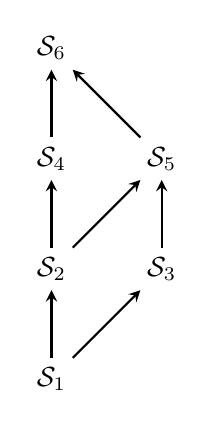
\begin{tikzpicture}[node distance=1.4cm]
\node (s6) {$\SS_6$};
\node (s4) [below of=s6] {$\SS_4$};
\node (s5) [right of=s4]  {$\SS_5$};
\node (s3) [below of=s5]  {$\SS_3$};
\node (s2) [below of=s4]  {$\SS_2$};
\node (s1) [below of=s2]  {$\SS_1$};

\draw [arrow] (s1) -- (s2);
\draw [arrow] (s2) -- (s4);
\draw [arrow] (s4) -- (s6);

\draw [arrow] (s1) -- (s3);
\draw [arrow] (s3) -- (s5);
\draw [arrow] (s5) -- (s6);

\draw [arrow] (s2) -- (s5);
\end{tikzpicture}
\end{center}
    \caption{\textcolor{black}{Inclusion relations among the $\SS_i$ sets.}}
    \label{fig:casefig-just-si}
\end{figure}


\begin{figure}[ht!]
\begin{center}
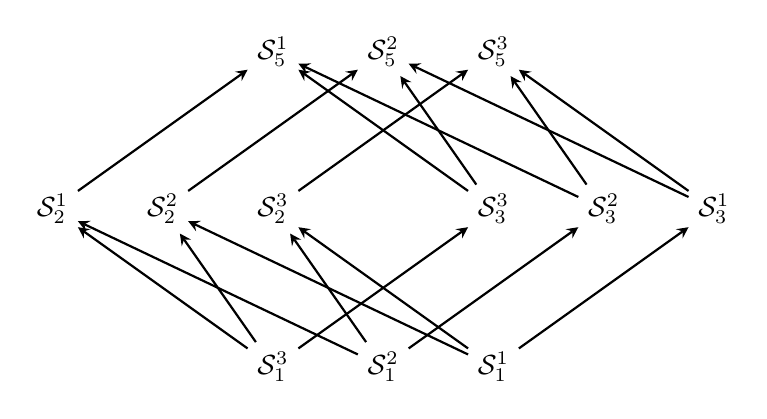
\begin{tikzpicture}[node distance=1.4cm]
\node (s51) {$\SS_5^1$};
\node (s52) [right of=s51]  {$\SS_5^2$};
\node (s53) [right of=s52]  {$\SS_5^3$};
\node (s21) [below of=s51, xshift=-2.8cm, yshift=-0.6cm] {$\SS_2^1$};
\node (s22) [right of=s21]  {$\SS_2^2$};
\node (s23) [right of=s22]  {$\SS_2^3$};
\node (s33) [right of=s23, xshift=1.4cm]  {$\SS_3^3$};
\node (s32) [right of=s33]  {$\SS_3^2$};
\node (s31) [right of=s32]  {$\SS_3^1$};
\node (s13) [below of=s21, xshift=2.8cm, yshift=-0.6cm]  {$\SS_1^3$};
\node (s12) [right of=s13]  {$\SS_1^2$};
\node (s11) [right of=s12]  {$\SS_1^1$};

\draw [arrow] (s13) -- (s21);
\draw [arrow] (s13) -- (s22);
\draw [arrow] (s13) -- (s33);

\draw [arrow] (s12) -- (s21);
\draw [arrow] (s12) -- (s23);
\draw [arrow] (s12) -- (s32);

\draw [arrow] (s11) -- (s22);
\draw [arrow] (s11) -- (s23);
\draw [arrow] (s11) -- (s31);

\draw [arrow] (s21) -- (s51);
\draw [arrow] (s22) -- (s52);
\draw [arrow] (s23) -- (s53);

\draw [arrow] (s33) -- (s51);
\draw [arrow] (s33) -- (s52);

\draw [arrow] (s32) -- (s51);
\draw [arrow] (s32) -- (s53);

\draw [arrow] (s31) -- (s52);
\draw [arrow] (s31) -- (s53);
\end{tikzpicture}
\end{center}
    \caption{Inclusion relations among some of the $\SS^j_i$ sets.}
    \label{fig:casefig}
\end{figure}


The sets $\SS^j_i$ satisfy three key properties that we state as Lemma~\ref{sjdiagsj}, Lemma~\ref{sdiags}, and Lemma~\ref{diagdag} and that we prove in Appendix~\ref{sec:proof-iff-equivalence}.
First, Lemma~\ref{sjdiagsj} says that we can map a gate from one of $\SS^1_i, \SS^2_i, \SS^3_i$ to another by conjugating the gate with a swap gate.

\begin{lemma}
\textcolor{black}{For all $i\in 1..6$,}
(1) $\overline{S}_{BC} \, \SS^1_i \, \overline{S}_{BC} =  \SS^1_i$, \ (2) $\oS_{AB} \, \SS^1_i \, \oS_{AB} = \SS^2_i$, \ (3) $\overline{S}_{AC} \, \SS^1_i \, \overline{S}_{AC} =  \SS^3_i$, \ (4) $\overline{S}_{AC} \, \SS^2_i \, \overline{S}_{AC} =  \SS^2_i$, \ (5) $\overline{S}_{BC} \, \SS^2_i \, \overline{S}_{BC} =  \SS^3_i$, and \ (6) $\oS_{AB} \, \SS^3_i \, \oS_{AB} =  \SS^3_i$.
\label{sjdiagsj}
\end{lemma} 

Second, Lemma~\ref{sdiags} says that conjugating a gate with a swap gate preserves the number of 2-qubit neighbor gates and the number of 2-qubit unrestricted gates used in an implementation.  Lemma~\ref{sdiags}  also states how to change each component gate when conjugating with a swap gate.

\begin{lemma}
For $k \in \{\ AB, \ AC, \ BC\ \}$, a 3-qubit gate $D$ can be implemented with $m$ 2-qubit 
% neighbor (unrestricted) 
gates as $D = \overline{U_1}_{i_1} \, \overline{U_2}_{i_2} \, \dots \, \overline{U_m}_{i_m}$ if and only if 
$\overline{S}_{k} \, D \, \overline{S}_{k}$ 
can be implemented with $m$ 2-qubit % neighbor (unrestricted) 
gates as $\overline{S}_{k} \, D \, \overline{S}_{k} = \overline{V_1}_{j_1} \, \overline{V_2}_{j_2} \, \dots \, \overline{V_m}_{j_m}$. Specifically, we have the following table.
% ranging $p$ from 1 to m, %\begin{enumerate}
%    \item for $k=BC$, we have if $i_p = BC$ then $V_p = S \, U_p \, S$ and $j_p = BC$, if $i_p = AC$ then $V_p =  U_p$ and $j_p = AB$, and if $i_p = AB$ then $V_p = U_p$ and $j_p = AC$.
%    \item for $k=AC$, we have if $i_p = BC$ then $V_p = S \, U_p \, S$ and $j_p = AB$, if $i_p = AC$ then $V_p =  S \, U_p \, S$ and $j_p = AC$, and if $i_p = AB$ then $V_p = S \, U_p \, S$ and $j_p = BC$.
%    \item for $k=AB$, we have if $i_p = BC$ then $V_p = U_p$ and $j_p = AC$, if $i_p = AC$ then $V_p =  U_p$ and $j_p = BC$, and if $i_p = AB$ then $V_p = S \, U_p \, S$ and $j_p = AB$.
%\end{enumerate}
\label{sdiags}
\end{lemma}
\vspace*{-0.4cm}
\[
\begin{array}{c|lcl}
\mbox{For mapping a product $D$ to:} & \multicolumn{3}{c}{\mbox{map each factor in $D$ as follows:}} \\
\hline \\[-3mm]
\multirow{3}{*}{$\oS_{BC}\ D\ \oS_{BC}$} 
& \oU_{BC} &\rightarrow& \overline{S\ U \ S}_{BC} \\
& \oU_{AC} &\rightarrow& \oU_{AB} \\
& \oU_{AB} &\rightarrow& \oU_{AC} \\ [1mm]
\hline \\[-3mm]
\multirow{3}{*}{$\oS_{AC}\ D\ \oS_{AC}$} 
& \oU_{BC} &\rightarrow& \overline{S\ U\ S}_{AB} \\
& \oU_{AC} &\rightarrow& \overline{S\ U\ S}_{AC} \\
& \oU_{AB} &\rightarrow& \overline{S\ U\ S}_{BC} \\ [1mm]
\hline \\[-3mm]
\multirow{3}{*}{$\oS_{AB}\ D\ \oS_{AB}$} 
& \oU_{BC} &\rightarrow& \oU_{AC} \\
& \oU_{AC} &\rightarrow& \oU_{BC} \\
& \oU_{AB} &\rightarrow& \overline{S\ U\ S}_{AB} \\ [1mm]
\hline
\end{array}
\]


When we combine Lemma~\ref{sjdiagsj} and Lemma~\ref{sdiags}, we see that for a given $i$, 
the least upper bounds for neighbor gates and unrestricted gates are the same across $\SS^1_i$, $\SS^2_i$, and $\SS^3_i$.



%For each 3-qubit diagonal gate $D = \diag{d_0, \  d_1, \ \dots \ , d_{7}}$, we borrow from \cite{shende2008cnot} the following definitions of  $\lambda_1(D)$, $\lambda_2(D)$, $\lambda_3(D)$, and $\xi(D)$. 
%\begin{equation*}
%\lambda_1(D) = \frac{d_{3} \, d_{0}}{d_{1} \, d_{2}}, \;\;\;\;\;\;
%\lambda_2(D) = \frac{d_{5} \, d_{0}}{d_{4} \, d_{1}}, \;\;\;\;\;\;
%\lambda_3(D) = \frac{d_{6} \, d_{0}}{d_{4} \, d_{2}}, \;\;\;\;\;\;
%\xi(D) = \frac{d_{7} \, d^2_{0}}{d_{4} \, d_{2} \, d_{1}}
%\end{equation*}
%We use the above to define the sets $\SS_1$ to $\SS_6$ and $\SS^k_5$ as follows,
%assuming that $i,j,k$ are distinct numbers in the set $\{1,2,3\}$.
%\begin{eqnarray*}
%\SS_1 &=& \{\ D \;|\; \exists i, j, k: (\xi(D) = \lambda_i(D)) \wedge (\lambda_j(D) = \lambda_k(D) = 1)\ \} \\
%\SS_2 &=& \{\ D \;|\; \exists i, j, k: (\xi(D) = \lambda_i(D) \cdot \lambda_j(D) ) \wedge (\lambda_k(D) = 1)\ \} \\
%\SS_3 &=& \{\ D \;|\; \exists i, j, k: (\xi(D) = \lambda_i(D)) \wedge (\lambda_j(D) = \lambda_k(D))\ \} \\
%\SS_4 &=& \{\ D \;|\; \exists i, j, k: \xi(D) = \lambda_i(D) \cdot \lambda_j(D) \cdot \lambda_k(D)\ \} \\
%\SS_5 &=& \{\ D \;|\; \exists i, j, k: \xi(D) = \lambda_i(D) \cdot \lambda_j(D) \ / \ \lambda_k(D)\ \} \\
%\SS^k_5 &=& \{\ D \;|\; \exists i, j: \xi(D) = \lambda_i(D) \cdot \lambda_j(D) \ / \ \lambda_k(D)\ \} \\
%\SS_6 &=& \mbox{the set of 3-qubit, diagonal unitaries}
%\end{eqnarray*}
% \begin{itemize}
%    \item $D \in \SS_1$ $\Leftrightarrow$ $\exists$ $a$, $b$, $c$: $S(D) = (a, 1, 1; a)$.
%    \item $D \in \SS_2$ $\Leftrightarrow$ $\exists$ $a$, $b$, $c$: $S(D) = (a, b, 1; ab)$.
%    \item $D \in \SS_3$ $\Leftrightarrow$ $\exists$ $a$, $b$, $c$: $S(D) = (a, b, b; a)$.
%    \item $D \in \SS_4$ $\Leftrightarrow$ $\exists$ $a$, $b$, $c$: $S(D) = (a, b, c; abc)$.
%    \item $D \in \SS_5$ $\Leftrightarrow$ $\exists$ $a$, $b$, $c$: $S(D) = (a, b, c; ab/c)$. Specifically, $D \in S^i_5$ % $\Leftrightarrow$ $c = \lambda_i(D)$.
%     \item $D \in \SS_6$ for every $S(D)$.
% \end{itemize}

Third, the dagger operation will not change the set to which a 3-qubit diagonal gate belongs. 
\begin{lemma}
A 3-qubit diagonal gate $D \in \SS^j_i$ if and only if $D^\dag \in \SS^j_i$. 
\label{diagdag}
\end{lemma} 

\paragraph{Examples.}
Here are examples of elements of the sets $\SS_1, \SS_2, \SS_3$.
First, for the 3-qubit gate $\CC{-I} = \diag{1, \ 1, \ 1, \ 1, \ 1, \ 1, \ -1, \ -1}$, we have that 
$d_{0} d_3 = d_{1} d_2$, $d_0 d_{5} = d_{1} d_4$, and $d_0 d_{7} = d_1 d_{6}$. From this, we conclude that $\CC{-I} \in \SS_1$. 
%\textcolor{blue}{According to Table~\ref{tab:numberoftwoqubit}, for implementing $D_1$, the least upper bound of 2-qubit neighbor gates is 1, and the least upper bound of 2-qubit neighbor of 2-qubit unrestricted gates is 1. }

%$\lambda_1(D_1) = 1$, $\lambda_2(D_1) = 1$, $\lambda_3(D_1) = -1$, and $\xi(D_1) = -1$. 
%According to Lemma~\ref{optlemmaneighbor1}, there exists one 2-qubit gate $U_1 = \diag{1, \ 1, \ 1, \ -1}$, such that $D = \overline{U_1}_{AB}$. It is optimal because $D$ cannot be implemented without 2-qubit gates.

For the gate $\C{Z \otimes Z} = \diag{1, \ 1, \ 1, \ 1, \ 1, \ -1, \ -1, \ 1}$, we have that $d_0 d_3 = d_1 d_2$ and $d_4 d_7 = d_5 d_6$. Also, we have that $d_0 d_7 = d_3 d_4$ and $d_1 d_6 = d_2 d_5$. From this, we conclude that
$\C{Z \otimes Z} \in \SS_2 \cap \SS_3$, but also that $\C{Z \otimes Z} \not \in \SS_1$. 
%\textcolor{blue}{According to Table~\ref{tab:numberoftwoqubit}, for implementing $\C{Z \otimes Z}$, the least upper bound of 2-qubit neighbor gates is 2, and the least upper bound of 2-qubit neighbor of 2-qubit unrestricted gates is 2. }
% According to Lemma~\ref{optlemmaneighbor2}, there exist two 2-qubit gates $U_1 = \diag{1, \ 1, \ 1, \ -1}$ and $U_2 = \diag{1, \ 1, \ 1, \ -1}$, such that $D = \overline{U_1}_{AB} \, \overline{U_2}_{AC}$. It is optimal because $D$ cannot be implemented using one 2-qubit gate.

If we change $-1$ to $i$ in $\C{Z \otimes Z}$, we get the gate 
$D_3 = \diag{1, \ 1, \ 1, \ 1, \ 1, \ i, \ i, \ 1}$, and we have $d_0 d_7 = d_3 d_4$ and $d_1 d_6 = d_2 d_5$.
%$\lambda_1(D_3) = 1$, $\lambda_2(D_3) = i$, $\lambda_3(D_3) = i$, and $\xi(D_3) = 1$. 
From this, we conclude that $D_3 \in \SS_3$.
Similarly, we can easily check that $D_3 \not \in \SS_2$. 
%\textcolor{blue}{According to Table~\ref{tab:numberoftwoqubit}, for implementing $D_3$, the least upper bound of 2-qubit neighbor gates is 3, and the least upper bound of 2-qubit neighbor of 2-qubit unrestricted gates is 3. }
% According to Lemma~\ref{optlemmaneighbor3}, there exist three 2-qubit neighbor gates $U_1 = S \, \C{X} \, S$, $U_2 = \diag{1, \ 1, \ 1, \ i}$, and $U_3 = S \, \C{X} \, S$, such that $D = \overline{U_1}_{BC} \, \overline{U_2}_{AB} \, \overline{U_1}_{BC}$. It is optimal because $D$ cannot be implemented using two 2-qubit gates.

For the gate $\C{S \otimes S^\dag} = \diag{1, \ 1, \ 1, \ 1, \ 1, \ -i, \ i, \ 1}$, and we have $d_0 d_3 = d_1 d_2$ and $d_4 d_7 = d_5 d_6$. 
From this, we conclude that $\C{S \otimes S^\dag} \in \SS_2$.
Similarly, we can easily check that $\C{S \otimes S^\dag} \not \in \SS_3$.
%\textcolor{blue}{According to Table~\ref{tab:numberoftwoqubit}, for implementing $D_4$, the least upper bound of 2-qubit neighbor gates is 2, and the least upper bound of 2-qubit neighbor of 2-qubit unrestricted gates is 2. }

\paragraph{Examples from Section~\ref{sec:programming-with-neighbor-gates}.}
Now we turn to the gates from Section~\ref{sec:programming-with-neighbor-gates}.
In Examples~\ref{sec:example-ccu-ab-bc} and~\ref{sec:example-ccu-ac-bc} % 2.1 and 2.2
we considered the 3-qubit gate $\CC{X}$, which can be conjugated with $I \otimes I \otimes H$ to give the diagonal gate $\CC{Z} = \diag{1, \ 1, \ 1, \ 1, \ 1, \ 1, \ 1, \ -1}$.
We have $\CC{Z} \not\in \SS_4$ because $d_0 d_3 d_5 d_6 = 1 \neq -1 = d_1 d_2 d_4 d_7$. Also, $\CC{Z} \not\in \SS^1_5$ because $d_0 d_3 d_4 d_7 = -1 \neq 1 = d_1 d_2 d_5 d_6$. Similarly, we can easily check that $\CC{Z} \not\in \SS^2_5$ and $\CC{Z} \not\in \SS^3_5$.
%$\lambda_1(\CC{Z}) = 1$, $\lambda_2(\CC{Z}) = 1$, $\lambda_3(\CC{Z}) = 1$, and $\xi(\CC{Z}) = -1$. 
So, $\CC{Z} \not\in \SS_4 \cup \SS_5$. 
%\textcolor{blue}{According to Table~\ref{tab:numberoftwoqubit}, for implementing $\CC{Z}$, the least upper bound of 2-qubit neighbor gates is 6 as shown in Examples~\ref{sec:example-ccu-ab-bc} and~\ref{sec:example-ccu-ac-bc}, and the least upper bound of 2-qubit neighbor of 2-qubit unrestricted gates is 5 as shown in Equation~\ref{eq:quantum-compilation-scheme-for-ccu-with-two-controls}. }

In Examples~\ref{sec:example-ccw-ac-bc-detw-1} and~\ref{sec:example-ccw-ab-bc-detw-1}
we considered $\CC{R_z(\alpha)} = \diag{1, \ 1, \ 1, \ 1, \ 1, \ 1, \ e^{-i\frac{\alpha}{2}}, \ e^{i\frac{\alpha}{2}}}$.
We have $\CC{R_z(\alpha)} \in \SS^3_5 \subseteq \SS_5$ because 
$d_0 d_1 d_6 d_7 = d_2 d_3 d_4 d_5$.
%$\lambda_1(\CC{R_z(\alpha)}) = 1$, $\lambda_2(\CC{R_z(\alpha)}) = 1$, $\lambda_3(\CC{R_z(\alpha)}) = e^{-i\alpha/2}$, and $\xi(\CC{R_z(\alpha)}) = e^{i\alpha/2}$. 
Similarly, we can easily check that $\CC{R_z(\alpha)} \not \in \SS_3 \cup \SS_4 \cup \SS^1_5 \cup \SS^2_5$. 
%\textcolor{blue}{According to Table~\ref{tab:numberoftwoqubit}, for implementing $\CC{R_z(\alpha)}$, the least upper bound of 2-qubit neighbor gates is 4, and the least upper bound of 2-qubit neighbor of 2-qubit unrestricted gates is 4 as shown in Example~\ref{sec:example-ccw-ac-bc-detw-1}. We will prove the optimality of Example~\ref{sec:example-ccw-ab-bc-detw-1} later in Section~\ref{sec:our-example-circuits-are-optimal}.}

In Example~\ref{sec:example-diag-on-ab-bc}
we considered the 3-qubit diagonal gate $W = \diag{1, \ 1, \ 1, \ -1, \ 1, \ i, \ i, \ 1}$.
We have $W \in \SS_4 \cap \SS_5$ because 
$d_0 d_3 d_5 d_6 = d_1 d_2 d_4 d_7$, and also 
$d_0 d_3 d_4 d_7 = d_1 d_2 d_5 d_6$.
%$\lambda_1(W) = -1$, $\lambda_2(W) = i$, $\lambda_3(W) = i$, and $\xi(W) = 1$. 
Similarly, we can easily check that $W \not \in \SS_2 \cup \SS_3$.
%\textcolor{blue}{According to Table~\ref{tab:numberoftwoqubit}, for implementing $W$, the least upper bound of 2-qubit neighbor gates is 4, and the least upper bound of 2-qubit neighbor of 2-qubit unrestricted gates is 3 as shown in Example~\ref{sec:example-diag-on-ab-bc}. }

% In Section~\ref{sec:toffoli-requires-six-neighbor-gates}, we will show their implementations we proposed in Section~\ref{sec:programming-with-neighbor-gates} are optimal. 

% Also, because we can change the implemented qubits of the first gate by applying $S$ gates, we only discuss the implementation where the first gate is on qubits $B$ and $C$. We omit other cases because (1) they have the same characteristics after applying $S$ gates, and (2) their implementation can be derived by applying $S$ gates backward.




%This is because according to Lemma~\ref{}, applying the $S$ gates keeps $D \in S_i$ and the same gate count in the implementation, but changes the implemented qubits for each gate and the order of $\lambda_j(D)$ in $S(D)$.

 
%This is because by using the $S$ gates, we can transform one implementation  

%This is because (1) for each implementation, applying $S$ gates can change the first gate to be on qubits $B$ and $C$; (2) if one sub-case of $D \in S_i$ can be implemented by a combination where the first gate is on qubits $B$ and $C$, then by applying the $S$ gates to such an implementation, we can obtain other sub-cases. 


\section{The Expressiveness of Four Neighbor Gates}
%\section{Toffoli Requires Six Neighbor Gates}
\label{sec:toffoli-requires-six-neighbor-gates}

In this section, we state two theorems on the expressiveness of four neighbor gates.
We begin with Theorem~\ref{lem:s4-s5-if-and-only-if-product-of-four-neighbor-gates}, which says that a 3-qubit diagonal gate $D$ belongs to subsets of $\SS_4 \cup \SS_5$ if and only if
$D$ can be implemented using particular products of four neighbor gates. 
This is significant because some 3-qubit diagonal gates, such as $\CC{R_z(\alpha)}$, are in one of the subsets of $\SS_4 \cup \SS_5$ but not the others, as we saw in Section~\ref{sec:sets-of-3-qubit-diagonal-gates}. 

\begin{theorem}
\label{lem:s4-s5-if-and-only-if-product-of-four-neighbor-gates}
Suppose $D$ is a 3-qubit diagonal gate.
\begin{enumerate}
\itemsep0em 
\item % was: lemma5.3.3
We have $D \in \SS_4 \cup \SS^1_5$ if and only if
there exist four 2-qubit gates $U_1$, $U_2$, $U_3$, $U_4$, such that $\overline{U_1}_{AC} \, \overline{U_2}_{AB} \, \overline{U_3}_{AC} \, \overline{U_4}_{AB} = D$.

\item % was: lemma5.3.2
We have $D \in \SS_4 \cup \SS^2_5$ if and only if
there exist four 2-qubit gates $U_1$, $U_2$, $U_3$, $U_4$ such that $\overline{U_1}_{BC} \, \overline{U_2}_{AB} \, \overline{U_3}_{BC} \, \overline{U_4}_{AB} = D$.

\item % was: lemma5.3.1
We have $D \in \SS_4 \cup \SS^3_5$ if and only if
there exist four 2-qubit gates $U_1$, $U_2$, $U_3$, $U_4$ such that $\overline{U_1}_{BC} \, \overline{U_2}_{AC} \, \overline{U_3}_{BC} \, \overline{U_4}_{AC} = D$.
\end{enumerate}

\end{theorem}
%
% Here, we prove Theorem~\ref{lem:s4-s5-if-and-only-if-product-of-four-neighbor-gates} by proving the properties in the order (3), (2), (1).
%Here is a summary of those proof steps.
% and the key idea is a series of if and only if statements. 
% The key idea is to prove Theorem~\ref{lem:s4-s5-if-and-only-if-product-of-four-neighbor-gates}.

%(3). We first transform $D \in \SS_4 \cup \SS^3_5$ into the form $\CC{\diag{d_0, \ d_1}}$, which can implemented using the same product as for $D$. Second, according to \cite{YuYing15,palsberg2024optimal}, $\CC{\diag{d_0, \ d_1}}$ can be implemented by such a product if and only if $d_0 = d_1$ or $d_0 d_1 = 1$, which is equivalent to $D \in  \SS_4 \cup \SS^3_5$.  

% From the above, we have the Theorem~\ref{lem:s4-s5-if-and-only-if-product-of-four-neighbor-gates}.(3).
%From Theorem~\ref{lem:s4-s5-if-and-only-if-product-of-four-neighbor-gates}.(3), we easily derive Theorem~\ref{lem:s4-s5-if-and-only-if-product-of-four-neighbor-gates}.(2) and Theorem~\ref{lem:s4-s5-if-and-only-if-product-of-four-neighbor-gates}.(1).



We prove Theorem~\ref{lem:s4-s5-if-and-only-if-product-of-four-neighbor-gates} by first proving Property (3) through a sequence of if-and-only-if statements. First, $D \in \SS_4 \cup \SS^3_5$ if and only if for particular $d_0', d_1'$, we have that $\CC{\diag{d_0', d_1'}}$ satisfies $d_0'd_1' = 1$ or $d_0' = d_1'$. Then we use Lemma~\ref{lemma6.4} to see that $\CC{\diag{d_0', d_1'}}$ satisfies this constraint if and only if $\CC{\diag{d_0', d_1'}}$ can be implemented by a particular combination of four neighbor gates. Finally, we use Lemma~\ref{sdiags} to transform this combination of neighbor gates to a product that both has the desired form and equals $D$. After we are done with proving Proving (3), we use Lemma~\ref{sjdiagsj} and Lemma~\ref{sdiags} to derive Properties~(1)--(2) from Property~(3). 



\begin{proof}{\sc (Theorem~\ref{lem:s4-s5-if-and-only-if-product-of-four-neighbor-gates})}\ \
Suppose we have a 3-qubit diagonal gate $D = \diag{d_0, d_1, d_2, d_3, d_4, d_5, d_6, d_7}$.
We will prove the three properties in the order (3), (2), (1).  

Property (3).
We reason as follows.
\begin{eqnarray}
D \in \SS_4 \cup \SS^3_5 
&\Longleftrightarrow&
d_0 d_3 d_5 d_6 = d_1 d_2 d_4 d_7 \;\;\vee\;\; d_0 d_1 d_6 d_7 = d_2 d_3 d_4 d_5 
\nonumber \\
&\Longleftrightarrow&
\frac{d_6 \, d_0}{d_2 \, d_4} = 
\frac{d_7 \, d_1}{d_3 \, d_5}
\;\;\vee\;\;
\frac{d_6 \, d_0}{d_2 \, d_4} \cdot \frac{d_7 \, d_1}{d_3 \, d_5} = 1
\nonumber \\
&\Longleftrightarrow&
\exists\ \mbox{2-qubit gates}\ V_1, V_2, V_3, V_4: 
\nonumber \\
&& \;\;\;\;
\overline{V_1}_{AC} \, \overline{V_2}_{BC} \, \overline{V_3}_{AC} \, \overline{V_4}_{BC} = \CC{\diag{\frac{d_6 \, d_0}{d_2 \, d_4}, \, \frac{d_7 \, d_1}{d_3 \, d_5}}} 
\nonumber \\
&\Longleftrightarrow&
\exists\ \mbox{2-qubit gates}\ V_1, V_2, V_3, V_4: 
\nonumber \\
&& \;\;\;\;
\oS_{AB}\ \overline{V_1}_{AC} \, \overline{V_2}_{BC} \, \overline{V_3}_{AC} \, \overline{V_4}_{BC}\ \oS_{AB} = \oS_{AB}\ \CC{\diag{\frac{d_6 \, d_0}{d_2 \, d_4}, \, \frac{d_7 \, d_1}{d_3 \, d_5}}}\ \oS_{AB} 
\nonumber \\
&\Longleftrightarrow&
\exists\ \mbox{2-qubit gates}\ V_1, V_2, V_3, V_4: 
\nonumber \\
&& \;\;\;\;
\overline{V_1}_{BC} \, \overline{V_2}_{AC} \, \overline{V_3}_{BC} \, \overline{V_4}_{AC} = \CC{\diag{\frac{d_6 \, d_0}{d_2 \, d_4}, \, \frac{d_7 \, d_1}{d_3 \, d_5}}} 
\nonumber \\
&\Longleftrightarrow&
\exists\ \mbox{2-qubit gates}\ U_1, U_2, U_3, U_4: 
\nonumber
\\
&& \;\;\;\;
\overline{U_1}_{BC} \, \overline{U_2}_{AC} \, \overline{U_3}_{BC} \, \overline{U_4}_{AC} = D
\label{eq:u1-u2-u3-u4-equals-d}
\end{eqnarray}
In the first step, we use the definitions of 
$D$, $\SS_4$, $\SS^3_5$.
In the third step, we use Lemma~\ref{lemma6.4}.
In the fifth step, we use Lemma~\ref{sdiags}.
In the sixth step, we define 
$W_1$ = $\diag{d_0, \, d_1, \, d_2, \, d_3}$ and $W_4$ = $\diag{1, \, 1, \, d_4 / d_0, \, d_5 / d_1}$, and then we use
$U_1 = W_1 V_1$ and $U_2 = V_2$ and $U_3 = V_3$ and $U_4 = V_4 W_4$.
This is sufficient to complete the proof of Property (3) because we have:
%
\begin{eqnarray}
\overline{W_1}_{BC} \, \CC{\diag{\frac{d_6 \, d_0}{d_2 \, d_4}, \, \frac{d_7 \, d_1}{d_3 \, d_5}}} \, \overline{W_4}_{AC}
% \nonumber \\
&=&
\diag{d_0, \, d_1, \, d_2, \, d_3, \,
      d_0, \, d_1, \, d_2, \, d_3} 
\nonumber \\
&& \diag{1, 1, 1, 1, 1, 1, \frac{d_6 \, d_0}{d_2 \, d_4}, \, \frac{d_7 \, d_1}{d_3 \, d_5}}
\nonumber \\
&&
\diag{1, 1, 1, 1, d_4 / d_0, \, d_5 / d_1, \,  d_4 / d_0, \, d_5 / d_1} 
\nonumber \\
&=&
\diag{d_0, d_1, d_2, d_3, d_4, d_5, d_6, d_7}
\nonumber \\
&=&
D
\nonumber
\end{eqnarray}

Property (2). 
We reason as follows.
\begin{eqnarray}
D \in \SS_4 \cup \SS^2_5 
&\Longleftrightarrow&
\oS_{BC}\ D\ \oS_{BC} \in \SS_4 \cup \SS^3_5
\nonumber \\
&\Longleftrightarrow&
\exists\ \mbox{2-qubit gates}\ V_1, V_2, V_3, V_4: 
\nonumber
\\
&& \;\;\;\;
\overline{V_1}_{BC} \, \overline{V_2}_{AC} \, \overline{V_3}_{BC} \, \overline{V_4}_{AC} = \oS_{BC}\ D\ \oS_{BC}
\nonumber \\
&\Longleftrightarrow&
\exists\ \mbox{2-qubit gates}\ V_1, V_2, V_3, V_4: 
\nonumber
\\
&& \;\;\;\;
\oS_{BC}\ \overline{V_1}_{BC} \, \overline{V_2}_{AC} \, \overline{V_3}_{BC} \, \overline{V_4}_{AC} \, \oS_{BC} = D
\nonumber \\
&\Longleftrightarrow&
\exists\ \mbox{2-qubit gates}\ V_1, V_2, V_3, V_4: 
\nonumber
\\
&& \;\;\;\;
\overline{S\ V_1\ S}_{BC} \, \overline{V_2}_{AB} \, 
\overline{S\ V_3\ S}_{BC} \, \overline{V_4}_{AB} = D
\nonumber \\
&\Longleftrightarrow&
\exists\ \mbox{2-qubit gates}\ U_1, U_2, U_3, U_4: 
\nonumber
\\
&& \;\;\;\;
\overline{U_1}_{BC} \, \overline{U_2}_{AB} \, 
\overline{U_3}_{BC} \, \overline{U_4}_{AB} = D
\end{eqnarray}
%
In the first step, we use Lemma~\ref{sjdiagsj}.
In the second step, we use Property (3).
In the fourth step, we use Lemma~\ref{sdiags}.


% According to Lemma~\ref{sdiags}, $D = \overline{U_1}_{BC} \, \overline{U_2}_{AB} \, \overline{U_3}_{BC} \, \overline{U_4}_{AB}$ is valid if and only if \\ $\overline{S}_{BC} \, D \, \overline{S}_{BC} = \overline{S \, U_1 \, S}_{BC} \, \overline{U_2}_{AC} \, \overline{S \, U_3 \, S}_{BC} \, \overline{U_4}_{AC}$ is valid. From this, according to Property (3), we know that $\overline{S}_{BC} \, D \, \overline{S}_{BC} = \overline{S \, U_1 \, S}_{BC} \, \overline{U_2}_{AC} \, \overline{S \, U_3 \, S}_{BC} \, \overline{U_4}_{AC}$ is valid if and only if $\overline{S}_{BC} \, D \, \overline{S}_{BC} \in \SS_4 \cup \SS^3_5$. According to Lemma~\ref{sjdiagsj}, we conclude that $\overline{U_1}_{BC} \, \overline{U_2}_{AB} \, \overline{U_3}_{BC} \, \overline{U_4}_{AB} = D$ if and only if $D \in \SS_4 \cup \SS^2_5$.

Property (1). 
We reason as follows.
\begin{eqnarray}
D \in \SS_4 \cup \SS^1_5 
&\Longleftrightarrow&
\oS_{AB}\ D\ \oS_{AB} \in \SS_4 \cup \SS^2_5
\nonumber \\
&\Longleftrightarrow&
\exists\ \mbox{2-qubit gates}\ V_1, V_2, V_3, V_4: 
\nonumber
\\
&& \;\;\;\;
\overline{V_1}_{BC} \, \overline{V_2}_{AB} \, \overline{V_3}_{BC} \, \overline{V_4}_{AB} = \oS_{AB}\ D\ \oS_{AB}
\nonumber \\
&\Longleftrightarrow&
\exists\ \mbox{2-qubit gates}\ V_1, V_2, V_3, V_4: 
\nonumber
\\
&& \;\;\;\;
\oS_{AB}\ \overline{V_1}_{BC} \, \overline{V_2}_{AB} \, \overline{V_3}_{BC} \, \overline{V_4}_{AB} \, \oS_{AB} = D
\nonumber \\
&\Longleftrightarrow&
\exists\ \mbox{2-qubit gates}\ V_1, V_2, V_3, V_4: 
\nonumber
\\
&& \;\;\;\;
\overline{V_1}_{AC} \, 
\overline{S\ V_2\ S}_{AB} \, 
\overline{V_3}_{AC} \, 
\overline{S\ V_4\ S}_{AB} = D
\nonumber \\
&\Longleftrightarrow&
\exists\ \mbox{2-qubit gates}\ U_1, U_2, U_3, U_4: 
\nonumber
\\
&& \;\;\;\;
\overline{U_1}_{AC} \, \overline{U_2}_{AB} \, 
\overline{U_3}_{AC} \, \overline{U_4}_{AB} = D
\nonumber
\end{eqnarray}
%
In the first step, we use Lemma~\ref{sjdiagsj}.
In the second step, we use Property (2).
In the fourth step, we use Lemma~\ref{sdiags}.
%
% Property (1). According to Lemma~\ref{sdiags}, $D = \overline{U_1}_{AC} \, \overline{U_2}_{AB} \, \overline{U_3}_{AC} \, \overline{U_4}_{AB}$ is valid if and only if $\oS_{AB} \, D \, \oS_{AB} = \overline{U_1}_{BC} \, \overline{S \, U_2 \, S}_{AB} \, \overline{U_3}_{BC} \, \overline{S \, U_4 \, S}_{AB}$ is valid. From this, according to Property (2), we know that $\oS_{AB} \, D \, \oS_{AB} = \overline{U_1}_{BC} \, \overline{S \, U_2 \, S}_{AB} \, \overline{U_3}_{BC} \, \overline{S \, U_4 \, S}_{AB}$  is valid if and only if  $\oS_{AB} \, D \, \oS_{AB} \in \SS_4 \cup \SS^2_5$. According to Lemma~\ref{sjdiagsj}, we conclude that $\overline{U_1}_{AC} \, \overline{U_2}_{AB} \, \overline{U_3}_{AC} \, \overline{U_4}_{AB} = D$ if and only if $D \in \SS_4 \cup \SS^1_5$.
\end{proof}


Next, we state Theorem~\ref{nearest neighbor4}, which says that 
the following four classes of 3-qubit diagonal gates are equivalent:
(1) $\SS_4 \cup \SS_5$,
(2) those implemented with four neighbor gates, 
(3) those implemented with five neighbor gates, and
(4) those implemented with four unrestricted gates.  
%Theorem~\ref{nearest neighbor4} shows the equivalences among the following four classes of 3-qubit diagonal gates: 
% (1) $\SS_4 \cup \SS_5$,
% (2) those implemented by four neighbor gates, 
% (3) those implemented by five neighbor gates, and
% (4) those implemented by four unrestricted gates. 

\begin{theorem} 
\label{nearest neighbor4}
Suppose $D$ is a 3-qubit diagonal gate. The following conditions on $D$ are equivalent.
\begin{enumerate}
\itemsep0em 
    \item $D \in \SS_4 \cup \SS_5$.
    \item There exist four 2-qubit gates $U_1$, $U_2$, $U_3$, $U_4$, such that $\overline{U_1}_{i_1} \, \overline{U_2}_{i_2} \, \overline{U_3}_{i_1} \, \overline{U_4}_{i_2} = D$, where $i_1$, $i_2$ $\in \{\ AB, \ AC, \ BC\ \}$.
    \item There exist five 2-qubit gates $W_1$, $W_2$, $W_3$, $W_4$, $W_5$, such that $\overline{W_1}_{j_1} \, \overline{W_2}_{j_2} \, \overline{W_3}_{j_1} \, \overline{W_4}_{j_2} \, \overline{W_5}_{j_1} = D$, where $j_1$, $j_2 \in \{\ AB, \ AC, \ BC\ \}$.
    \item There exist four 2-qubit gates $V_1$, $V_2$, $V_3$, $V_4$, such that $\overline{V_1}_{k_1} \, \overline{V_2}_{k_2} \, \overline{V_3}_{k_3} \, \overline{V_4}_{k_4} = D$, where $k_1$, $k_2$, $k_3$, $k_4 \in \{\ AB, \ AC, \ BC\ \}$.
\end{enumerate}
\end{theorem}

Notice that in Theorem~\ref{nearest neighbor4}, each of Properties (2)--(3) uses just two indices, which means that the matrix products use neighbor gates.  In contrast, Property (4) uses four indices.

We give the proof of Theorem~\ref{nearest neighbor4} below, but first we outline the idea of the proof.
The centerpiece of the proof is Table~\ref{tbl:sec5}, which summarizes key properties that we prove in a suite of lemmas. Notice that in Table~\ref{tbl:sec5}, each row has a structure that is similar to the four items in Theorem~\ref{nearest neighbor4}.
Specifically, the first column of Table~\ref{tbl:sec5} has a subset of $\SS_4 \cup \SS_5$, the third column has a product of four neighbor gates, the fourth column has a product of five neighbor gates, and the fifth column has a product of four unrestricted gates.
Additionally, the second column lists the two qubits that the first gate in each of the products in columns 3--5 works on. 

\renewcommand{\arraystretch}{1.4}
\begin{table}[htb]
\centering
\caption{Summary of our lemmas in Theorem~\ref{nearest neighbor4}.}
\label{tbl:sec5}
\begin{tabular}{c|c|c|c|c}
\toprule
$D$ & 1$^{st}$ gate  & Four neighbor gates  & Five neighbor gates & Four gates \\

\midrule

$\SS_4 \cup \SS^3_5$ &
\multirow{2}{*}{$BC$}  &  $\overline{U_1}_{BC} \, \overline{U_2}_{AC} \, \overline{U_3}_{BC} \, \overline{U_4}_{AC} \ $ &  $\overline{W_1}_{BC} \, \overline{W_2}_{AC}$ & 
$\overline{V_1}_{BC} \, \overline{V_2}_{AC}$\\ 
\cline{1-1} \cline{3-3}
$\SS_4 \cup \SS^2_5$ &  &  $\overline{U_1}_{BC} \, \overline{U_2}_{AB} \, \overline{U_3}_{BC} \, \overline{U_4}_{AB}$ & $\overline{W_3}_{BC} \, \overline{W_4}_{AC} \, \overline{W_5}_{BC}$ & 
$\overline{V_3}_{AB} \, \overline{V_4}_{BC}$ \\ 

\midrule
%%%%%%%%%%%%%%%%%%%%%%%%%%%%%%%%%%%%%

$\SS_4 \cup \SS^2_5$ &
\multirow{2}{*}{$AB$}  &  $\overline{U_1}_{AB} \, \overline{U_2}_{BC} \, \overline{U_3}_{AB} \, \overline{U_4}_{BC} \ $ & $\overline{W_1}_{AB} \, \overline{W_2}_{BC}$ & 
$\overline{V_1}_{AB} \, \overline{V_2}_{BC}$\\ 
\cline{1-1} \cline{3-3}
$\SS_4 \cup \SS^1_5$ & &  $\overline{U_1}_{AB} \, \overline{U_2}_{AC} \, \overline{U_3}_{AB} \, \overline{U_4}_{AC}$ & $\overline{W_3}_{AB} \, \overline{W_4}_{BC} \, \overline{W_5}_{AB}$ & 
$\overline{V_3}_{AC} \, \overline{V_4}_{AB}$ \\ 

\midrule
%%%%%%%%%%%%%%%%%%%%%%%%%%%%%%%%%%%%%

$\SS_4 \cup \SS^3_5$ &
\multirow{2}{*}{$AC$}  &  $\overline{U_1}_{AC} \, \overline{U_2}_{BC} \, \overline{U_3}_{AC} \, \overline{U_4}_{BC} \ $ & $\overline{W_1}_{AC} \, \overline{W_2}_{BC}$ & 
$\overline{V_1}_{AC} \, \overline{V_2}_{BC}$ \\ 
\cline{1-1} \cline{3-3}
$\SS_4 \cup \SS^1_5$ & & $\overline{U_1}_{AC} \, \overline{U_2}_{AB} \, \overline{U_3}_{AC} \, \overline{U_4}_{AB}$ & $\overline{W_3}_{AC} \, \overline{W_4}_{BC} \, \overline{W_5}_{AC}$ & 
$\overline{V_3}_{AB} \, \overline{V_4}_{AC}$ \\
\bottomrule
\end{tabular}
\end{table}

The key idea of Table~\ref{tbl:sec5} is to show different approaches to implementing gates in the three sets 
$\SS_4 \cup \SS^1_5$,
$\SS_4 \cup \SS^2_5$, and
$\SS_4 \cup \SS^3_5$.
For example, if we want to consider an implementation of a gate in $\SS_4 \cup \SS^3_5$, and we want the first gate to operate on qubits $BC$, then Table~\ref{tbl:sec5} suggests three different ways of doing it. The first implementation uses four neighbor gates, and the second uses five neighbor gates, 
while the third, in column ``Four gates'', uses four unrestricted gates.  

% The proof of Theorem~\ref{nearest neighbor4} relies on
Table~\ref{tbl:sec5} is based on two key lemmas. 
First, in Appendix~\ref{sec:reduction-to-few-cases}, 
Lemma~\ref{4gate} shows a reduction from arbitrary products of four 2-qubit unrestricted gates to the nine cases listed in the third and fifth columns of Table~\ref{tbl:sec5}.
Lemma~\ref{5nearest neighbor} shows a reduction from arbitrary products of five 2-qubit neighbor gates to the three cases listed in the fourth column of Table~\ref{tbl:sec5}.
Together, Lemma~\ref{4gate} and Lemma~\ref{5nearest neighbor} enable us to focus on the products listed in Table~\ref{tbl:sec5} when we discuss a product using four or five 2-qubit gates in Theorem~\ref{nearest neighbor4}.



% From the above, we prove Theorem~\ref{nearest neighbor4} by proving  (1) $\Rightarrow$ (2) $\Rightarrow$ (3) $\Rightarrow$ (4) $\Rightarrow$ (1).

\begin{proof}{\sc (Theorem~\ref{nearest neighbor4})}\ \
%
%
%
%We prove Theorem~\ref{nearest neighbor4} by proving (1) $\Rightarrow$ (2) $\Rightarrow$ (3) $\Rightarrow$ (4) $\Rightarrow$ (1).
%Here is a summary of those proof steps.
%The implication (1) $\Rightarrow$ (2) is immediate from Theorem~\ref{lem:s4-s5-if-and-only-if-product-of-four-neighbor-gates}, using $\SS_5 = \SS^1_5 \cup \SS^2_5 \cup \SS^3_5$.
%The implication (2) $\Rightarrow$ (3) is immediate by using $I$ as the fifth gate.
%The implication (4) $\Rightarrow$ (1) relies on the reasoning that is akin to what we use in the proof of Theorem~\ref{lem:s4-s5-if-and-only-if-product-of-four-neighbor-gates}.
%
We will prove (1) $\Rightarrow$ (2) $\Rightarrow$ (3) $\Rightarrow$ (4) $\Rightarrow$ (1).
    
Condition (1) $\Rightarrow$ Condition (2). \ 
Immediate from Theorem~\ref{lem:s4-s5-if-and-only-if-product-of-four-neighbor-gates}, using $\SS_5 = \SS^1_5 \cup \SS^2_5 \cup \SS^3_5$.

% If $D \in \SS_4 \cup \SS_5 = \SS_4 \cup S^1_5 \cup S^2_5 \cup S^3_5$, then according to Lemma~\ref{lem:s4-s5-if-and-only-if-product-of-four-neighbor-gates}, there exist four 2-qubit gates $V_1$, $V_2$, $V_3$, $V_4$, such that $\overline{V_1}_{BC} \, \overline{V_2}_{AC} \, \overline{V_3}_{BC} \, \overline{V_4}_{AC} = D$, or $\overline{V_1}_{BC} \, \overline{V_2}_{AB} \, \overline{V_3}_{BC} \, \overline{V_4}_{AB} = D$, or $\overline{V_1}_{AC} \, \overline{V_2}_{AB} \, \overline{V_3}_{AC} \, \overline{V_4}_{AB} = D$.
    
Condition (2) $\Rightarrow$ Condition (3). \ We use $I$ as the fifth gate.
    % If there exist four 2-qubit gates $V_1$, $V_2$, $V_3$, and $V_4$, such that either $\overline{V_1}_{BC} \, \overline{V_2}_{AC} \, \overline{V_3}_{BC} \, \overline{V_4}_{AC} = D$ or $\overline{V_1}_{BC} \, \overline{V_2}_{AB} \, \overline{V_3}_{BC} \, \overline{V_4}_{AB} = D$, then according to Lemma~\ref{lemma5.4}, there exist five 2-qubit gates $W_1$, $W_2$, $W_3$, $W_4$, and $W_5$, such that $\overline{W_1}_{BC} \, \overline{W_2}_{AC} \, \overline{W_3}_{BC} \, \overline{W_4}_{AC} \, \overline{W_5}_{BC} = D$.
    
Condition (3) $\Rightarrow$ Condition (4). \ 
    Suppose there exist five 2-qubit gates $W_1$, $W_2$, $W_3$, $W_4$, $W_5$, such that
    $\overline{W_1}_{j_1} \, \overline{W_2}_{j_2} \, \overline{W_3}_{j_1} \, \overline{W_4}_{j_2} \, \overline{W_5}_{j_1} = D$, where $j_1$, $j_2 \in \{\ AB, \ AC, \ BC\ \}$.
    According to Lemma~\ref{5nearest neighbor}, we can assume that the product is one of the three cases in the fourth column in Table~\ref{tbl:sec5}.
    We will consider each of those three cases in turn.
    
    First, if $j_1 = BC$ and $j_2 = AC$, then from Lemma~\ref{lemma:diag-5-to-4}, we have that there exist four 2-qubit gates $V_1$, $V_2$, $V_3$, $V_4$, such that $\overline{V_1}_{BC} \, \overline{V_2}_{AC} \, \overline{V_3}_{AB} \, \overline{V_4}_{BC} = D$.  


Second, if $j_1 = AB$ and $j_2 = BC$, then according to Lemma~\ref{sdiags}, we know that $\overline{S}_{BC} \, \overline{S}_{AC} \, D \, \overline{S}_{AC} \, \overline{S}_{BC} = \overline{W_1}_{BC} \, \overline{S \, W_2 \, S}_{AC} \, \overline{W_3}_{BC} \, \overline{S \, W_4 \, S}_{AC} \, \overline{W_5}_{BC}$. According to Lemma~\ref{lemma:diag-5-to-4}, there exist four 2-qubit gates $V_1$, $V_2$, $V_3$, $V_4$, such that $\overline{S}_{BC} \, \overline{S}_{AC} \, D \, \overline{S}_{AC} \, \overline{S}_{BC} = \overline{V_1}_{BC} \, \overline{V_2}_{AC} \, \overline{V_3}_{AB} \, \overline{V_4}_{BC}$. From this, according to Lemma~\ref{sdiags}, we know that $D = \overline{V_1}_{AB} \, \overline{S \, V_2 \, S}_{BC} \, \overline{S \, V_3 \, S}_{AC} \, \overline{V_4}_{AB}$. 

Third, if $j_1 = AC$ and $j_2 = BC$, then according to Lemma~\ref{sdiags}, we know that $\oS_{AB} \, D \, \oS_{AB} = \overline{W_1}_{BC} \, \overline{W_2}_{AC} \, \overline{W_3}_{BC} \, \overline{W_4}_{AC} \, \overline{W_5}_{BC}$. According to Lemma~\ref{lemma:diag-5-to-4}, there exist four 2-qubit gates $V_1$, $V_2$, $V_3$, $V_4$, such that $\oS_{AB} \, D \, \oS_{AB} = \overline{V_1}_{BC} \, \overline{V_2}_{AC} \, \overline{V_3}_{AB} \, \overline{V_4}_{BC}$. From this, according to Lemma~\ref{sdiags}, we know that $D = \overline{V_1}_{AC} \, \overline{V_2}_{BC} \, \overline{S \, V_3 \, S}_{AB} \, \overline{V_4}_{AC}$. 

Thus, in all three cases, we get the desired conclusion.

Condition (4) $\Rightarrow$ Condition (1). \ 
    Suppose there exist four 2-qubit gates $V_1$, $V_2$, $V_3$, $V_4$, such that  $\overline{V_1}_{k_1} \, \overline{V_2}_{k_2} \, \overline{V_3}_{k_3} \, \overline{V_4}_{k_4} = D$, where $k_1$, $k_2$, $k_3$, $k_4 \in \{\ AB, \ AC, \ BC\ \}$.
    From Lemma~\ref{4gate} we have that we can assume that
    the product is one of the nine cases in the third and fifth columns in Table~\ref{tbl:sec5}.
    We will show the three cases in the fifth column in detail here. The first case we will consider is the one where 
    $k_1=BC$, $k_2 = AC$, $k_3 = AB$, and $k_4 = BC$.
    %From this and Lemma~\ref{lemma5.2}, we conclude that $D \in \SS_4 \cup S^2_5 \cup S^3_5 \subseteq \SS_4 \cup \SS_5$. 
    Let us write $D = \diag{d_0, d_1, \dots, d_7}$ as $D = \outer{0}{0} \otimes D_0 + \outer{1}{1} \otimes D_1$, where $D_0 = \diag{d_0, d_1, d_2, d_3}$ and $D_1 = \diag{d_4, d_5, d_6, d_7}$. From the assumption about $D$, we have that 
\begin{equation}
\overline{V_2}_{AC} \, \overline{V_3}_{AB} = \outer{0}{0} \otimes (V_1^\dag \, D_0 \, V_4^\dag)  + \outer{1}{1} \otimes (V_1^\dag \, D_1 \, V_4^\dag)
\label{eq:5.2}
\end{equation}

By Equation~(\ref{eq:5.2}), according to Lemma~\ref{lemmaa.24}, there exist four 1-qubit gates $P_0$, $P_1$, $Q_0$, $Q_1$, such that $\overline{V_2}_{AC} \, \overline{V_3}_{AB} = \outer{0}{0} \otimes P_0 \otimes Q_0 + \outer{1}{1} \otimes P_1 \otimes Q_1$, and we have that
\begin{equation}
    D_0 = V_1 \, (P_0 \otimes Q_0) \, V_4 \quad\quad
D_1 = V_1 \, (P_1 \otimes Q_1) \, V_4
\label{eq:5.3}
\end{equation}

By Equation~(\ref{eq:5.3}), we conclude that
\begin{equation}
    D^\dag_0 \, D_1 = V^\dag_4 \, (P^\dag_0P_1 \otimes Q^\dag_0Q_1) \, V_4
\label{eq:5.4}
\end{equation}

By Lemma~\ref{lemmaa.5}, there exist four complex numbers $a$, $b$, $p$, $q$, such that $\eigenvalues{P^\dag_0P_1 \otimes Q^\dag_0Q_1} = (ap, \ bp, \ aq, \ bq)$. From this and by Equation~(\ref{eq:5.4}), we have that
\begin{eqnarray}
    \eigenvalues{D^\dag_0 \, D_1} & = & (\frac{d_{4}}{d_{0}}, \ \frac{d_{5}}{d_{1}}, \ \frac{d_{6}}{d_{2}}, \ \frac{d_{7}}{d_{3}} ) \nonumber \\
    = \quad \eigenvalues{V^\dag_4 \, (P^\dag_0P_1 \otimes Q^\dag_0Q_1) \, V_4} & = & (ap, \ bp, \ aq, \ bq)
\label{eq:5.5}
\end{eqnarray}

According to Equation~(\ref{eq:5.5}), we conclude that for $\eigenvalues{D^\dag_0 \, D_1}$, there exists the multiplication of two eigenvalues equal to the multiplication of the other two eigenvalues. Thus, we have the following three cases. \ (1) If $d_0d_1d_6d_7 = d_2d_3d_4d_5$, we conclude that $D \in \SS^3_5$. \ (2) If $d_0d_2d_5d_7 = d_1d_3d_4d_6$, we conclude that $D \in \SS^2_5$. \ (3) If $d_0d_3d_5d_6 = d_1d_2d_4d_7$, we conclude that $D \in \SS_4$. As a result, we conclude that $D \in \SS_4 \cup \SS^2_5 \cup \SS^3_5 \subseteq \SS_4 \cup \SS_5$.

For the second case where $k_1=AB$, $k_2 = BC$, $k_3 = AC$, and $k_4 = AB$, according Lemma~\ref{sdiags}, we have that $\overline{S}_{BC} \, \overline{S}_{AC} \, D \, \overline{S}_{AC} \, \overline{S}_{BC} = \overline{V_1}_{BC} \, \overline{S \, V_2 \, S}_{AC} \, \overline{S \, V_3 \, S}_{AB} \, \overline{V_4}_{BC}$. From the analysis of the first case, we conclude that $\overline{S}_{BC} \, \overline{S}_{AC} \, D \, \overline{S}_{AC} \, \overline{S}_{BC} \in \SS_4 \cup \SS^2_5 \cup \SS^3_5$. According to Lemma~\ref{sjdiagsj}, we conclude that $D \in \SS_4 \cup \SS^1_5 \cup \SS^2_5 \subseteq \SS_4 \cup \SS_5$.

For the third case where $k_1=AC$, $k_2 = BC$, $k_3 = AB$, and $k_4 = AC$, according Lemma~\ref{sdiags}, we have that $\oS_{AB} \, D \, \oS_{AB} = \overline{V_1}_{BC} \, \overline{V_2}_{AC} \, \overline{S \, V_3 \, S}_{AB} \, \overline{V_4}_{BC}$. From the analysis of the first case, we conclude that $\oS_{AB} \, D \, \oS_{AB} \in \SS_4 \cup \SS^2_5 \cup \SS^3_5$. According to Lemma~\ref{sjdiagsj}, we conclude that $D \in \SS_4 \cup \SS^1_5 \cup \SS^3_5 \subseteq \SS_4 \cup \SS_5$. 

For the other six cases in the third column, three of them can be derived according to Theorem~\ref{lem:s4-s5-if-and-only-if-product-of-four-neighbor-gates}, and the other three cases can be derived by symmetry. 
For the first case where $k_1= AB$, $k_2 = AC$, $k_3 = AB$, and $k_4 = AC$, if
$D = \overline{V_1}_{AB} \overline{V_2}_{AC} \overline{V_3}_{AB} \overline{V_4}_{AC}$, then we have that $D^\dag = \overline{V^\dag_4}_{AC} \overline{V^\dag_3}_{AB} \overline{V^\dag_2}_{AC} \overline{V^\dag_1}_{AB}$. According to Theorem~\ref{lem:s4-s5-if-and-only-if-product-of-four-neighbor-gates} property (1), we conclude that $D^\dag \in \SS_4 \cup \SS^1_5$. According to Lemma~\ref{diagdag}, we conclude that $D \in \SS_4 \cup \SS^1_5$.

For the second case where $k_1=AB$, $k_2 = BC$, $k_3 = AB$, and $k_4 = BC$, if
$D = \overline{V_1}_{AB} \overline{V_2}_{BC} \overline{V_3}_{AB} \overline{V_4}_{BC}$, then we have that $D^\dag = \overline{V^\dag_4}_{BC} \overline{V^\dag_3}_{AB} \overline{V^\dag_2}_{BC} \overline{V^\dag_1}_{AB}$. According to Theorem~\ref{lem:s4-s5-if-and-only-if-product-of-four-neighbor-gates} property (2), we conclude that $D^\dag \in \SS_4 \cup \SS^2_5$. According to Lemma~\ref{diagdag}, we conclude that $D \in \SS_4 \cup \SS^2_5$.

For the third case where $k_1= AC$, $k_2 = BC$, $k_3 = AC$, and $k_4 = BC$, if
$D = \overline{V_1}_{AC} \overline{V_2}_{BC} \overline{V_3}_{AC} \overline{V_4}_{BC}$, then we have that $D^\dag = \overline{V^\dag_4}_{BC} \overline{V^\dag_3}_{AC} \overline{V^\dag_2}_{BC} \overline{V^\dag_1}_{AC}$. According to Theorem~\ref{lem:s4-s5-if-and-only-if-product-of-four-neighbor-gates} property (3), we conclude that $D^\dag \in \SS_4 \cup \SS^3_5$. According to Lemma~\ref{diagdag}, we conclude that $D \in \SS_4 \cup \SS^3_5$.

The above three cases, along with six others that can be derived according to Theorem~\ref{lem:s4-s5-if-and-only-if-product-of-four-neighbor-gates}, lead to the overall conclusion that $D \in \SS_4 \cup \SS_5$.
\end{proof}

% \paragraph{The circuit in Section~\ref{sec:example-ccu-ac-bc} is optimal.}

% \paragraph{The circuit in Section~\ref{sec:example-ccw-ab-bc-detw-1} is optimal.}

% Moreover, we will show in Section~\ref{sec:full-characterization-of-3-qubit-diagonal-gates} that three neighbor gates cannot make $\CC{R_z(\alpha)} \in \SS_3$. 

\section{Characterization of All 3-qubit Diagonal Gates}
\label{sec:full-characterization-of-3-qubit-diagonal-gates}

In this section, we \textcolor{black}{first} state two theorems that \textcolor{black}{give upper bounds on the} number of 2-qubit gates needed to implement a 3-qubit diagonal gate.
We begin with Theorem~\ref{thm:optimal-neighbor-implementation-of-3-qubit-diagonal-gates}, which focuses on neighbor gates.

% Here, we generalize the discussion from $\CC{X}$ to all 3-qubit diagonal gates.  For every 3-qubit diagonal gate $D$, Theorem~\ref{thm:optimal-neighbor-implementation-of-3-qubit-diagonal-gates} presents a tight bound on the number of needed neighbor gates, and Theorem~\ref{thm:optimal-implementation-of-3-qubit-diagonal-gates} presents a tight bound on the number of needed unrestricted gates. We summarize the optimal bounds in Table~\ref{tab:numberoftwoqubit}, and we present detailed proofs for each statement in Appendices. We first state Theorem~\ref{thm:optimal-neighbor-implementation-of-3-qubit-diagonal-gates} 

\begin{theorem}
\label{thm:optimal-neighbor-implementation-of-3-qubit-diagonal-gates}
Suppose $D$ is a 3-qubit diagonal gate. % We have the following statements for $D$.
\begin{enumerate}
\itemsep0em 
    \item We have $D \in \SS_1$ if and only if $D$ can be implemented with one 2-qubit neighbor gate.
    \item We have $D \in \SS_2$ if and only if $D$ can be implemented with two 2-qubit neighbor gates.
    \item We have $D \in \SS_2 \cup \SS_3$ if and only if $D$ can be implemented with three 2-qubit neighbor gates.
    \item We have $D \in \SS_4 \cup \SS_5$ if and only if $D$ can be implemented with four 2-qubit neighbor gates.
    \item We have $D \in \SS_6$ if and only if $D$ can be implemented with six 2-qubit neighbor gates.
\end{enumerate}
\end{theorem}

Notice that $\SS_2$ appears twice in Theorem~\ref{thm:optimal-neighbor-implementation-of-3-qubit-diagonal-gates} because we state if-and-only-if properties.
\textcolor{black}{
Specifically, in the forwards direction, both 2 and 3 are upper bounds for $\SS_2$, while in the backwards direction, we characterize accurately which gates can be implemented with two 2-qubit neighbor gates and with three 2-qubit neighbor gates.}
%、
In Appendix~\ref{sec:optimal-neighbor-thm}, we prove each if-and-only-if property by proving the two directions separately. For the left-to-right direction, we pick a 3-qubit diagonal gate from the given subset and then implement it with neighbor gates.
For the right-to-left direction, we first assume that a three-qubit diagonal gate $D$ equals the product of some 2-qubit neighbor gates. Then we discuss which restrictions each neighbor gate must satisfy to make this equation valid. The neighbor gates satisfy those restrictions simultaneously, which let us derive the subset to which $D$ belongs.
%In Appendix~\ref{sec:optimal-neighbor-thm}, we prove each property by first supposing that the product of 2-qubit neighbor gates equals diagonal gate and then deducing characteristics of each of the 2-qubit gates.

Next, we state Theorem~\ref{thm:optimal-implementation-of-3-qubit-diagonal-gates}, which focuses on unrestricted gates.

\begin{theorem}
\label{thm:optimal-implementation-of-3-qubit-diagonal-gates}
Suppose $D$ is a 3-qubit diagonal gate. % We have the following statements for $D$.
\begin{enumerate}
\itemsep0em 
    \item We have $D \in \SS_1$ if and only if $D$ can be implemented with one 2-qubit unrestricted gate.
    \item We have $D \in \SS_2$ if and only if $D$ can be implemented with two 2-qubit unrestricted gates.    
    \item We have $D \in \SS_3 \cup \SS_4$ if and only if $D$ can be implemented with three 2-qubit unrestricted gates.
    \item We have $D \in \SS_4 \cup \SS_5$ if and only if $D$ can be implemented with four 2-qubit unrestricted gates.
    \item We have $D \in \SS_6$ if and only if $D$ can be implemented with five 2-qubit unrestricted gates.
    
\end{enumerate}
\end{theorem}

Notice that $\SS_4$ appears twice in Theorem~\ref{thm:optimal-implementation-of-3-qubit-diagonal-gates}, which is because we state if-and-only-if properties.
%
In Appendix~\ref{sec:optimal-unrestricted-thm}, we prove Theorem~\ref{thm:optimal-implementation-of-3-qubit-diagonal-gates}.
In the left-to-right direction, the cases of $\SS_1$, $\SS_2$, $\SS_3$, and $\SS_5$ are immediate from Theorem~\ref{thm:optimal-neighbor-implementation-of-3-qubit-diagonal-gates}.
In contrast, we give a separate proof of the case of $\SS_4$, akin to the proof of the case of $\SS_4$ in Theorem~\ref{thm:optimal-neighbor-implementation-of-3-qubit-diagonal-gates}, 
and we also give a separate proof of the case of $\SS_6$.
In the right-to-left direction, we do the proof in a manner similar to that of Theorem~\ref{thm:optimal-neighbor-implementation-of-3-qubit-diagonal-gates}, but without neighbor restrictions.

%Theorem~\ref{thm:optimal-implementation-of-3-qubit-diagonal-gates} is valid because according to Theorem~\ref{thm:optimal-neighbor-implementation-of-3-qubit-diagonal-gates}.  Section~\ref{sec:quantum-concepts}, we have that $\SS_1 \subseteq \SS_2 \subseteq \SS_4 \subseteq \SS_6$ and $\SS_1 \subseteq \SS_3 \subseteq \SS_5 \subseteq \SS_6$, but $\SS_2 \not \subset \SS_3$, $\SS_3 \not \subset \SS_4$, and $\SS_4 \not \subset \SS_5$.  

% Here, we ignore the products using two 2-qubit unrestricted gates and the products using one 2-qubit unrestricted gate. This is because if we implement at most two 2-qubit gates on three pairs $AB$, $BC$, and $AC$, then there is no difference between the unrestricted and neighbor architecture, which is the same as Theorem~\ref{thm:optimal-neighbor-implementation-of-3-qubit-diagonal-gates}.(1) and Theorem~\ref{thm:optimal-neighbor-implementation-of-3-qubit-diagonal-gates}.(2). 

\textcolor{black}{
Now we use the upper bounds in Theorem~\ref{thm:optimal-neighbor-implementation-of-3-qubit-diagonal-gates} and Theorem~\ref{thm:optimal-implementation-of-3-qubit-diagonal-gates}, along with examples from Section~\ref{sec:sets-of-3-qubit-diagonal-gates}, to prove Corollary~\ref{cor:least-upper-bounds}, which states least upper bounds.
}
%\textcolor{blue}{We use the examples from Section~\ref{sec:sets-of-3-qubit-diagonal-gates} to prove this.}

\begin{corollary}
\label{cor:least-upper-bounds}
\textcolor{black}{
Table~\ref{tab:numberoftwoqubit} states the least upper bounds on the number of 2-qubit gates needed to implement any gate in $\SS_1,\ldots,\SS_6$.
}
\end{corollary}

\begin{proof}
\textcolor{black}{
For $\SS_1$, according to Theorem~\ref{thm:optimal-neighbor-implementation-of-3-qubit-diagonal-gates}.(1), the upper bound on the number of 2-qubit neighbor gates is 1, and according to Theorem~\ref{thm:optimal-implementation-of-3-qubit-diagonal-gates}.(1), the upper bound on the number of 2-qubit unrestricted gates is 1. 
Because there exists a 3-qubit diagonal gate $\CC{-I} = \diag{1, \ 1, \ 1, \ 1, \ 1, \ 1, \ -1, \ -1} = \C{Z} \otimes I$, such that $\CC{-I} \in \SS_1$ and $\CC{-I}$ cannot be implemented without 2-qubit gates, we conclude that for $\SS_1$, the least upper bound on the number of 2-qubit neighbor gates is 1, and the least upper bound on the number of 2-qubit unrestricted gates is 1. 
}

\textcolor{black}{
For $\SS_2$, according to Theorem~\ref{thm:optimal-neighbor-implementation-of-3-qubit-diagonal-gates}.(2), the upper bound on the number of 2-qubit neighbor gates is 2, and according to Theorem~\ref{thm:optimal-implementation-of-3-qubit-diagonal-gates}.(2), the upper bound on the number of 2-qubit unrestricted gates is 2. 
Because there exists a 3-qubit diagonal gate $\C{Z \otimes Z} = \diag{1, \ 1, \ 1, \ 1, \ 1, \ -1, \ -1, \ 1}$, such that $\C{Z \otimes Z} \in \SS_2$ and $\C{Z \otimes Z} \notin \SS_1$, we conclude that $\C{Z \otimes Z}$ cannot be implemented with one 2-qubit neighbor gate according to Theorem~\ref{thm:optimal-neighbor-implementation-of-3-qubit-diagonal-gates}.(1) or one 2-qubit unrestricted gate according to Theorem~\ref{thm:optimal-implementation-of-3-qubit-diagonal-gates}.(1). Thus, for $\SS_2$, the least upper bound on the number of 2-qubit neighbor gates is 2, and the least upper bound on the number of 2-qubit unrestricted gates is 2. 
}

\textcolor{black}{
For $\SS_3$, according to Theorem~\ref{thm:optimal-neighbor-implementation-of-3-qubit-diagonal-gates}.(3), the upper bound on the number of 2-qubit neighbor gates is 3, and according to Theorem~\ref{thm:optimal-implementation-of-3-qubit-diagonal-gates}.(3), the upper bound on the number of 2-qubit unrestricted gates is 3. 
Because there exists a 3-qubit diagonal gate $D_3 = \diag{1, \ 1, \ 1, \ 1, \ 1, \ i, \ i, \ 1}$, such that $D_3 \in \SS_3$ and $D_3 \notin \SS_2$, we conclude that $D_3$ cannot be implemented with two 2-qubit neighbor gates according to Theorem~\ref{thm:optimal-neighbor-implementation-of-3-qubit-diagonal-gates}.(2) or two 2-qubit unrestricted gates according to Theorem~\ref{thm:optimal-implementation-of-3-qubit-diagonal-gates}.(2). Thus, for $\SS_3$, the least upper bound on the number of 2-qubit neighbor gates is 3, and the least upper bound on the number of 2-qubit unrestricted gates is 3. 
}

\textcolor{black}{
For $\SS_4$, according to Theorem~\ref{thm:optimal-neighbor-implementation-of-3-qubit-diagonal-gates}.(4), the upper bound on the number of 2-qubit neighbor gates is 4, and according to Theorem~\ref{thm:optimal-implementation-of-3-qubit-diagonal-gates}.(3), the upper bound on the number of 2-qubit unrestricted gates is 3. 
Because there exists a 3-qubit diagonal gate $W = \diag{1, \ 1, \ 1, \ -1, \ 1, \ i, \ i, \ 1}$ as shown in Example~\ref{sec:example-diag-on-ab-bc}, such that $W \in \SS_4$ and $W \notin \SS_2 \cup \SS_3$, we conclude that $W$ cannot be implemented with three 2-qubit neighbor gates according to Theorem~\ref{thm:optimal-neighbor-implementation-of-3-qubit-diagonal-gates}.(3) or two 2-qubit unrestricted gates according to Theorem~\ref{thm:optimal-implementation-of-3-qubit-diagonal-gates}.(2). Thus, for $\SS_4$, the least upper bound on the number of 2-qubit neighbor gates is 4, and the least upper bound on the number of 2-qubit unrestricted gates is 3. 
}

\textcolor{black}{
For $\SS_5$, according to Theorem~\ref{thm:optimal-neighbor-implementation-of-3-qubit-diagonal-gates}.(4), the upper bound on the number of 2-qubit neighbor gates is 4, and according to Theorem~\ref{thm:optimal-implementation-of-3-qubit-diagonal-gates}.(4), the upper bound on the number of 2-qubit unrestricted gates is 4. 
Because there exists a 3-qubit diagonal gate $\CC{R_z(\alpha)} = \diag{1, \ 1, \ 1, \ 1, \ 1, \ 1, \ e^{-i\frac{\alpha}{2}}, \ e^{i\frac{\alpha}{2}}}$ as shown in Examples~\ref{sec:example-ccw-ac-bc-detw-1} and~\ref{sec:example-ccw-ab-bc-detw-1}, such that $\CC{R_z(\alpha)}  \in \SS_5$ and $W \notin \SS_3 \cup \SS_4$, we conclude that $\CC{R_z(\alpha)}$ cannot be implemented with three 2-qubit neighbor gates according to Theorem~\ref{thm:optimal-neighbor-implementation-of-3-qubit-diagonal-gates}.(3) or three 2-qubit unrestricted gates according to Theorem~\ref{thm:optimal-implementation-of-3-qubit-diagonal-gates}.(3). Thus, for $\SS_5$, the least upper bound on the number of 2-qubit neighbor gates is 4, and the least upper bound on the number of 2-qubit unrestricted gates is 4. 
}

\textcolor{black}{
For $\SS_6$, according to Theorem~\ref{thm:optimal-neighbor-implementation-of-3-qubit-diagonal-gates}.(5), the upper bound on the number of 2-qubit neighbor gates is 6, and according to Theorem~\ref{thm:optimal-implementation-of-3-qubit-diagonal-gates}.(5), the upper bound on the number of 2-qubit unrestricted gates is 5. 
Because there exists a 3-qubit diagonal gate $\CC{Z} = \diag{1, \ 1, \ 1, \ 1, \ 1, \ 1, \ 1, \ -1}$, such that $\CC{Z}  \in \SS_6$ and $W \notin \SS_4 \cup \SS_5$, we conclude that $\CC{Z}$ cannot be implemented with four 2-qubit unrestricted gates according to Theorem~\ref{thm:optimal-implementation-of-3-qubit-diagonal-gates}.(4). Also, according to Theorem~\ref{nearest neighbor4}, we conclude that $\CC{Z}$ cannot be implemented with five 2-qubit neighbor gates. Thus, for $\SS_6$, the least upper bound on the number of 2-qubit neighbor gates is 6, and the least upper bound on the number of 2-qubit unrestricted gates is 5. 
}

\textcolor{black}{In summary, we have proved that Table~\ref{tab:numberoftwoqubit} states the least upper bounds on the number of 2-qubit gates needed to implement any gate in $\SS_1,\ldots,\SS_6$.}
\end{proof}

% KELI: The reason why we have properties (3) and (4), is because I add a sentence in Sec 3: each $S_i$ does not necessarily contain all the elements in the previous set. Though $\SS_5$ has a larger number as 5 than $\SS_4$ as 4, actually not all the elements in $\SS_4$ is contained in $\SS_5$, that is why we need to say $\SS_4$ twice in the theorem, because $\SS_4$ is not included in $\SS_5$, only $\SS_3$ is included in $\SS_5$.






%\begin{table}[htp]
%\centering
%\caption{Optimal bounds on the number of 2-qubit gates needed to implement $D$.}
%\label{tab:numberoftwoqubit}
%\begin{tabular}{c|c|c|c|c|c|c}
%\toprule
%\# of 2-qubit gates & $D \in \SS_1$ & $D \in \SS_2$ & $D \in \SS_3$ & $D \in \SS_4$ & $D \in \SS_5$ & $D \in \SS_6$ \\
%\midrule
%Neighbor gates & 1 & 2 & 3 & {\bf 4} & 4 & {\bf 6} \\
%\midrule
%Unrestricted gates & 1 & 2 & 3 & {\bf 3} & 4 & {\bf 5} \\
%\bottomrule
%\end{tabular}
%\end{table}


%\begin{table}[htp]
%\centering
%\caption{Optimal bounds on the number of 2-qubit gates needed to implement $D$.}
%\label{tab:numberoftwoqubit}
%\begin{tabular}{c|c|c|c|c|c|c}
%\toprule
%\# of 2-qubit gates & $D \in \SS_1$ & $D \in \SS_2$ & $D \in \SS_3$ & $D \in \SS_4$ & $D \in \SS_5$ & $D \in \SS_6$ \\
%\midrule
%Unrestricted & 1, Lm.~\ref{optlemmaneighbor1} & 2, Lm.~\ref{optlemmaneighbor2} & 3, Lm.~\ref{optlemma3} & 3, Lm.~\ref{optlemma3} & 4, Lm.~\ref{optlemma4} & 5, Lm.~\ref{optlemma5} \\
%\midrule
%Neighbor & 1, Lm.~\ref{optlemmaneighbor1} & 2, Lm.~\ref{optlemmaneighbor2} & 3, Lm.~\ref{optlemmaneighbor3} & 4, Lm.~\ref{optlemmaneighbor4} & 4, Lm.~\ref{optlemmaneighbor4} & 6, Lm.~\ref{optlemmaneighbor6} \\
%\bottomrule
%\end{tabular}
%\end{table}


\section{Our Example Circuits in Section~\ref{sec:programming-with-neighbor-gates} are Optimal}
\label{sec:our-example-circuits-are-optimal}


\paragraph{The Circuits in Examples~\ref{sec:example-ccu-ab-bc} and~\ref{sec:example-ccu-ac-bc} 
are optimal.}
Each of our circuits in Examples~\ref{sec:example-ccu-ab-bc} and~\ref{sec:example-ccu-ac-bc} 
implements $\CC{X}$ using six neighbor gates.  
Because $\CC{X}$ can be diagonalized using 1-qubit gates to $\CC{Z}$, the number of two-qubit neighbor gates needed to implement $\CC{X}$ is the same as for $\CC{Z}$. 
From Section~\ref{sec:sets-of-3-qubit-diagonal-gates}, we have that $\CC{Z} \not\in \SS_4 \cup \SS_5$.
From this and Theorem~\ref{nearest neighbor4}, specifically (3) $\Rightarrow$ (1), we conclude that five 2-qubit neighbor gates cannot make a Toffoli gate, so six neighbor gates are needed. 


\paragraph{The Circuit in Example~\ref{sec:example-ccw-ac-bc-detw-1} 
is optimal.}
Our circuit in Example~\ref{sec:example-ccw-ac-bc-detw-1} 
implements $\CC{R_z(\alpha)}$ using four neighbor gates.
From Section~\ref{sec:sets-of-3-qubit-diagonal-gates}, we have that 
$\CC{R_z(\alpha)} \in \SS^3_5 \subseteq \SS_5$, but $\CC{R_z(\alpha)} \not \in \SS_3 \cup \SS_4 \cup \SS^1_5 \cup \SS^2_5 $. 
From this, because $\SS_2 \subseteq \SS_4$, according to Theorem~\ref{thm:optimal-neighbor-implementation-of-3-qubit-diagonal-gates}.(3), we conclude that three 2-qubit neighbor gates cannot make a $\CC{R_z(\alpha)}$ gate, so four neighbor gates are needed. 

\paragraph{The Circuit in Example~\ref{sec:example-ccw-ab-bc-detw-1} 
is optimal.}
Our circuit in Example~\ref{sec:example-ccw-ab-bc-detw-1} 
implements $\CC{R_z(\alpha)}$ using five neighbor gates on $AB$ and $BC$. 
From Section~\ref{sec:sets-of-3-qubit-diagonal-gates}, we have that 
$\CC{R_z(\alpha)} \in \SS^3_5$, but $\CC{R_z(\alpha)} \not\in \SS_3 \cup \SS_4 \cup \SS^1_5 \cup S^2_5$.
From Theorem~\ref{lem:s4-s5-if-and-only-if-product-of-four-neighbor-gates}.(2) and 
$\CC{R_z(\alpha)} \not\in \SS_4 \cup \SS^2_5$, we have that we cannot implement 
$\CC{R_z(\alpha)}$ on $AB$ and $BC$ using four neighbor gates, so five neighbor gates on $AB$ and $BC$ are needed.  

% Also, we have that $\CC{R_z(-\alpha)} \in S^3_5$ and $\CC{R_z(-\alpha)} \not \in \SS_3 \cup \SS_4 \cup S^1_5 \cup S^2_5$. 
% According to Lemma~\ref{lem:s4-s5-if-and-only-if-product-of-four-neighbor-gates} property (2), we cannot implement either $\CC{R_z(\alpha)}$ or $\CC{R_z(-\alpha)}$ using this particular product of four neighbor gates on $AB$ and $BC$.  
%However, if $\CC{R_z(\alpha)}$ can be implemented by a product of four 2-qubit neighbor gates on $AB$ and $BC$, then we must have either $\CC{R_z(\alpha)}$ or $\CC{R_z(-\alpha)}$ can be implemented by this particular product in the property~(2). From this, we conclude that if we can do 2-qubit gates on $AB$ and $BC$, $\CC{R_z(\alpha)}$ cannot be implemented using four neighbor gates. 
% The same is valid for the case if we can do 2-qubit gates on $AB$ and $AC$.
% Thus, the circuit is optimal.

\paragraph{The Circuits in Example~\ref{sec:example-diag-on-ab-bc} 
is optimal.}
Our circuits in Example~\ref{sec:example-diag-on-ab-bc} 
implements $W$ using three unrestricted gates and four neighbor gates, respectively.
From Section~\ref{sec:sets-of-3-qubit-diagonal-gates}, we have that 
$W \in \SS_4 \cap \SS_5$, but $W \not \in \SS_2 \cup \SS_3$. 
From this and according to Theorem~\ref{thm:optimal-implementation-of-3-qubit-diagonal-gates}.(2), we conclude that two 2-qubit unrestricted gates cannot make a $W$ gate, so three unrestricted gates are needed.
Also, according to Theorem~\ref{thm:optimal-neighbor-implementation-of-3-qubit-diagonal-gates}.(3), we conclude that three 2-qubit neighbor gates cannot make a $W$ gate, so four neighbor gates are needed. 

%
\paragraph{The impact of qubit layout.}
Examples~\ref{sec:example-ccu-ab-bc} and~\ref{sec:example-ccu-ac-bc} along with Equation~(\ref{eq:quantum-compilation-scheme-for-ccx}) illustrate that the optimal number of 2-qubit gates for implementing a 3-qubit diagonal gate outside $\SS_4 \cup \SS_5$, depends on whether we allow unrestricted gates or only neighbor gates.
%
Similarly, Example~\ref{sec:example-diag-on-ab-bc} illustrates that the optimal number of 2-qubit gates for implementing a gate in $\SS_4$, but outside $\SS_2 \cup \SS_3$, depends on whether we allow unrestricted gates or only neighbor gates.
%
Examples~\ref{sec:example-ccw-ac-bc-detw-1} and~\ref{sec:example-ccw-ab-bc-detw-1} illustrate that the optimal number of 2-qubit neighbor gates for implementing a gate in $\SS_5$, but outside $\SS_3 \cup \SS_4$, depends on the qubit layout.


\section{Related Work}
\label{sec:related}

\paragraph{Least upper bounds for 3-qubit Diagonal Gates.} 
\cite{YuDuanYing13,YuYing15,palsberg2024optimal} studied 3-qubit diagonal gates of the form $\CC{\diag{d_0, \ d_1}}$.
They proved the following least upper bounds on the number of unrestricted gates needed in an implementation.
If $\CC{\diag{d_0, \ d_1}} \in \SS_1$, which happens when $d_0 = d_1$, then it can be implemented using one 2-qubit gate.  If $\CC{\diag{d_0, \ d_1}} \in \SS_5$ which happens when $d_0 \, d_1 = 1$ or  $d_0 = d_1$, then it can be implemented using four 2-qubit gates.  In general, if $\CC{\diag{d_0, \ d_1}} \in \SS_6$, then it can be implemented using five 2-qubit gates.
Our Theorem~\ref{thm:optimal-implementation-of-3-qubit-diagonal-gates} generalizes their results.

For any 3-qubit diagonal gate $D$, \cite{shende2008cnot} proved the following least upper bounds on the number of unrestricted $\C{X}$ gates needed in an implementation.  
If $D \in \SS_1$, then it can be implemented with two $\C{X}$ gates. If $D \in \SS_4$, then it can be implemented with five $\C{X}$ gates, a remarkable jump from the three gates that are sufficient if we can freely pick the 2-qubit gates. If $D \in \SS_5$, then it can be implemented with four $\C{X}$ gates. 
Notice that elements of $\SS_4$ require as most as many 2-qubit unrestricted gates as elements of $\SS_5$ according to Theorem~\ref{thm:optimal-implementation-of-3-qubit-diagonal-gates}, while, perhaps surprisingly, elements of $\SS_4$ require at least as many unrestricted $\C{X}$ gates as elements of $\SS_5$.
This is possible in part because $\SS_4 \not\subseteq \SS_5$ and $\SS_5 \not\subseteq \SS_4$.
If $D \in \SS_6$, then it can be implemented with six $\C{X}$ gates. 



\paragraph{Mapping Circuits to Neighbor Gates.} % Many recent papers consider nearest-neighbor architectures. 
%Some work designed innovative workflows for mapping quantum circuits to those 2-dimensional nearest neighbor architectures including grid and hexagon.
\cite{wille2014optimal} presented strategies for mapping a quantum circuit to a nearest-neighbor architecture by inserting swap gates. 
Many papers on this mapping problem have followed, 
including \cite{farghadan2017quantum} for a two-dimensional grid,
% \cite{farghadan2017quantum} proposed a flow for the physical design of quantum circuits on a two-dimensional grid. 
\cite{bhattacharjee2018novel,hattori2019mapping} for a two-dimensional architecture, and
\cite{chang2021mapping,datta2022mapping,datta2022nearest} for a two-dimensional hexagonal architecture.
%Some work tried to only consider inserting the SWAP gates optimally in the circuits which satisfied the nearest neighbor architecture constraints.
\cite{zhao2020switchable} studied how to map a variety of controlled gates to a nearest-neighbor architecture.  
\cite{duckering2021orchestrated} showed how to implement a Toffoli gate using eight $\C{X}$ neighbor gates.
\cite{park2023reducing} constructed a one-dimensional nearest-neighbor circuit for the quantum Fourier transform. 
None of those papers show optimality.



%\cite{hattori2019mapping} proposed a new approach to optimize the number of swap gates for a two-dimensional architecture.
%Other work designed end-to-end compilation schemes from high-level quantum applications to low-level neighbor gates.


%%%% \cite{biswal2018implementation} presented a quantum gate that is nearest-neighbor compliant with a unit quantum cost.


\section{Conclusion}

The Toffoli gate is a key building block for error-corrected quantum computers, and it is a key component of many quantum algorithms. For implementing a Toffoli gate, we consider common quantum architectures that have only neighbor gates, and we prove that six 2-qubit neighbor gates are necessary and sufficient. Moreover, we prove least upper bounds for implementing 3-qubit diagonal gates using neighbor gates and using unrestricted gates, respectively. We find that while the expressive power of four 2-qubit unrestricted gates is the same as four 2-qubit neighbor gates, the expressive power of five 2-qubit unrestricted gates is strictly more than five 2-qubit neighbor gates. 

Our results are independent of specific gate sets.
This implies that there is no gate set with 2-qubit gates and 1-qubit gates that supports that we use just five neighbor gates to implement a Toffoli gate.  
Rather, for any specific gate set, we must use at least six neighbor gates.

We see at least six directions for future work, which we discuss below.

%

\paragraph{Automation.}
Is it possible to automate our analysis by an SMT-solver or an automated theorem prover? Such an automation could provide more general insights for larger and more complex configurations that might be intractable to analyze manually.
%
\textcolor{black}{
\paragraph{ZX-calculus.}
Can some of our proofs be given more easily using ZX-calculus or ZH-calculus?
}

%

\paragraph{Limited gate sets.}
Actual quantum hardware typically supports only a limited gate set. 
How many neighbor gates are required
to implement a Toffoli gate under such hardware constraints? 

%

\paragraph{Asymptotic lower bounds.}
How many neighbor gates are required to implement an $n$-qubit Toffoli gates with $(n-1)$ controls?
\citeN{shende2008cnot} showed that we need at least $2n$ unrestricted $\C{X}$ gates, and we speculate that a lower bound on the number of neighbor $\C{X}$ gates will be even higher.

%

\paragraph{General 3-qubit gates.}
How many neighbor gates are required to implement any 3-qubit gate?  
\cite{chen2024one} showed that 11 unrestricted gates are sufficient, and we speculate that we need even more neighbor gates.
%
\textcolor{black}{
\paragraph{Non-neighbors.}
How many neighbor gates are required to implement a Toffoli gate on three qubits that are connected but where either none of them are neighbors or only two of them are neighbors?
One way to approach this case might be to use swap gates to bring two pairs of the qubits to be neighbors, resulting in the situation in Figure~\ref{fig:enter-label}.
}

\paragraph{Qubit mapping.}
How can our results be integrated into an algorithm for qubit mapping?

%

\paragraph{Different qubit technologies.}
Different qubit technologies have different constraints on ``which qubits are neighbors?''  In this paper, we have taken our motivation from a leading kind of quantum computer that uses superconducting qubits.  However, quantum computers based on trapped-ion qubits, spin qubits, and neutral-atom qubits come with different constraints.  This opens the question of how many 2-qubit gates are needed to implement a Toffoli gate on such computers.
\textcolor{black}{
For example, we can ask how many M{\o}lmer-S{\o}rensen gates are needed.}


\paragraph{Acknowledgements.} 
We are grateful to the anonymous reviewers for their many helpful suggestions that led us to improve the paper.
We are supported by the NSF QLCI program: grant number OMA-2016245.


%% We will uncomment the acknowledgment after the paper is accepted:
%% \paragraph{Acknowledgements.}  We thank Shuohao Ping and Zhuoyang (John) Ye for helpful comments on a draft of the paper.

\clearpage

\appendix

\section{Known Lemmas}
\label{sec:known-lemmas}

\begin{lemma} {\rm \cite[\textsc{Observation} 2]{shende2008cnot}}
For an $(n+1)$-qubit gate $V$, it commutes with $Z$ gates on qubit $i$ if and only if there exist two $n$-qubit gates $V_{0}$ and $V_{1}$, such that $V = \ket{0}\bra{0} \otimes V_{0} + \ket{1}\bra{1} \otimes V_{1}$ on qubit $i$.
\label{commutez}
\end{lemma}


\begin{lemma} {\rm \cite[\textsc{Theorem} 2.5.3]{horn2012matrix}}
For an n-qubit gate $V$, there exist $2^{n}$ complex numbers $d_0$, $d_1$, $\dots$, $d_{2^n-1}$ and one $n$-qubit gate $P$, where $\eigenvalues{V} = (d_0, \ d_1, \ \dots, \ d_{2^n-1})$, such that
\[ 
\Qcircuit @C=0.5em @R=0.6em {
 & \qw / & \gate{V}  &  \qw &  = &  & \qw /  &  \gate{P^\dag}  & \gate{\diag{d_0, \ d_1, \ \dots, \ d_{2^n-1}}}  & \gate{P} &\qw\\
}
\]
\label{lemmaspec}
\end{lemma}


\begin{lemma} 
For an n-qubit gate $V$, there exist $2^{n}$ complex numbers $d_0$, $d_1$, $\dots$, $d_{2^n-1}$ and one n-qubit gate $P$, where $\eigenvalues{V} = (d_0, \ d_1, \ \dots, \ d_{2^n-1})$, such that
\[ 
\Qcircuit @C=0.5em @R=0.6em {
& \qw / & \ctrl{2}  &  \qw &  &  & \qw / & \qw & \ctrl{2}  & \qw &\qw\\
&  &   &   & = &  &  &  &  & & \\
& \qw / & \gate{V}  &  \qw &   &  & \qw / &  \gate{P^\dag}  & \gate{\diag{d_0, \ d_1, \ \dots, \ d_{2^n-1}}}  & \gate{P} &\qw\\
}
\]
\label{lemmacontrolspec}
\end{lemma}

\begin{proof}
    One can easily prove this according to Lemma~\ref{lemmaspec}.
\end{proof}


\begin{lemma} {\rm \cite{paige1994history}}
For a 2-qubit gate $V$, there exist six 1-qubit gates $P_0$, $P_1$, $R_y(\theta_0)$, $R_y(\theta_1)$, $Q_0$, and $Q_1$ and three 2-qubit gates $P = \outer{0}{0} \otimes P_{0} + \outer{1}{1} \otimes P_{1}$, $R = R_y(\theta_0) \otimes \outer{0}{0} + R_y(\theta_1) \otimes \outer{1}{1}$, and $Q= \outer{0}{0} \otimes Q_{0} + \outer{1}{1} \otimes Q_{1}$, 
such that
\[ 
\Qcircuit @C=0.5em @R=0.4em {
  & \multigate{2}{V} & \qw &   &  & \gate{} \qwx[2]& \gate{R}      &\gate{} \qwx[2]&\qw\\
 &                  &     & = &       &          &                 &               &   \\
 &  \ghost{V}        & \qw &   & & \gate{Q}       & \gate{} \qwx[-2]&\gate{P}       &\qw\\
}
\]
\label{cosinesine}
\end{lemma}


\begin{lemma} {\rm \cite{shende2005synthesis}}
For two 1-qubit gates $V_{0}$ and $V_{1}$ and one 2-qubit gate $V = \outer{0}{0} \otimes V_{0} + \outer{1}{1} \otimes V_{1}$, there exist four 1-qubit gates $P$, $Q$, $R_{z}(\alpha_0)$, and $R_{z}(\alpha_1)$ and one 2-qubit gate $R = R_{z}(\alpha_0) \otimes \outer{0}{0} + R_{z}(\alpha_1) \otimes \outer{1}{1}$, such that
\[ 
\Qcircuit @C=0.5em @R=0.4em {
  & \gate{} \qwx[2] & \qw &   &  & \qw       & \gate{R}      &\qw            &\qw\\  
 & &     & = &  &             &                 &               &   \\
& \gate{V}       & \qw &   &  & \gate{Q}       & \gate{} \qwx[-2]&\gate{P}       &\qw\\
}
\]
\label{demultiplexing}
\end{lemma}


\begin{lemma} {\rm \cite[\textsc{Equation} 4]{shende2008cnot}}
    Suppose $d_0$, $d_1$ are two complex numbers. For $\C{\diag{d_0, \ d_1}}$, there exist one 1-qubit gate $P(\varphi)$ and one 2-qubit gate $\C{R_z(\alpha)}$, such that
\[ 
\Qcircuit @C=0.5em @R=0.4em {
 & \ctrl{2} & \qw &   &  &  \gate{P(\varphi)}           & \ctrl{2}    &\qw\\
 &                  &     & = &  &                &       &   \\
 & \gate{\diag{d_0, \ d_1}}       & \qw &   &  &  \qw  & \gate{R_z(\alpha)}  &\qw\\
}
\]
\label{lemmadiag}
\end{lemma}


%\begin{proof}
%We define $e^{i\varphi} = \sqrt{u_0u_1}$, $e^{i\alpha/2} = \sqrt{u_1/u_0}$ , and $e^{-i\alpha/2} = \sqrt{u_0/u_1}$. From this, we have 
%\begin{equation*}
%    \C{R_z(\alpha)} \cdot (p(\varphi) \otimes I) = 
%\begin{bmatrix}
%1 & 0 & 0 & 0 \\
%0 & 1 & 0 & 0 \\
%0 & 0 & e^{-i\alpha/2} & 0 \\
%0 & 0 & 0 & e^{i\alpha/2}
%\end{bmatrix}
%\begin{bmatrix}
%1 & 0 & 0 & 0 \\
%0 & 1 & 0 & 0 \\
%0 & 0 & e^{i\varphi} & 0 \\
%0 & 0 & 0 & e^{i\varphi}
%\end{bmatrix}
%=
%\begin{bmatrix}
%1 & 0 & 0 & 0 \\
%0 & 1 & 0 & 0 \\
%0 & 0 & u_0 & 0 \\
%0 & 0 & 0 & u_1
%\end{bmatrix}
%\end{equation*}
%\end{proof}

\begin{lemma}
For two n-qubit gates $V_0$ and $V_1$, we have
$V = \outer{0}{0} \otimes V_0 + \outer{1}{1} \otimes V_1 = \C{V_1V^\dag_0}\ (I \otimes V_0)$.
% and a 2-qubit gate $\Box(V) = \outer{0}{0} \otimes V_0 + \outer{1}{1} \otimes V_1$, 
%there exist 1-qubit gates $V_0$, $V^\dag_0V_1$, such that
%% we have 
%% $\Box(V) = (I \otimes V_0)\ \C{V^\dag_0V_1}$:
\[ 
\Qcircuit @C=0.5em @R=0.4em {
 & \qw & \gate{} \qwx[2] & \qw &   &  & \qw & \qw            & \ctrl{2}        &\qw \\
 &                  &     & & = &                &                 &    \\
 & \qw / & \gate{V}       & \qw &   & & \qw / & \gate{V_0}       & \gate{V^\dag_0V_1}&\qw\\
}
\]
\label{10control}
\end{lemma}


\begin{proof}
$\C{V_1V^\dag_0}\ (I \otimes V_0)
= 
(\outer{0}{0} \otimes I + \outer{1}{1} \otimes V_1V^\dag_0)\ 
(I \otimes V_0)
=
\outer{0}{0} \otimes V_0 + \outer{1}{1} \otimes V_1$.
\end{proof}

\begin{lemma} {\rm \cite[\textsc{Lemma} 6.1]{palsberg2024optimal}} For a 2-qubit gate $V$, either
\begin{itemize}
    \item $\exists\ket{y}:V (\ket{y}\otimes\ket{0})$ is entangled, or
    \item $\exists\ket{x}:\forall\ket{y}:\exists\ket{z}:V (\ket{y}\otimes\ket{0}) = \ket{x}\otimes\ket{z}$, or
    \item $\exists\ket{x}:\forall\ket{y}:\exists\ket{z}:V (\ket{y}\otimes\ket{0}) = \ket{z}\otimes\ket{x}$.
\end{itemize}
\label{lemma6.1}
\end{lemma}

\begin{lemma} {\rm \cite[\textsc{Lemma} 6.4]{palsberg2024optimal}} Suppose $d_0$, $d_1$ are complex numbers such that $|d_0| = |d_1| = 1$. There exist 2-qubit unitaries $U_1$, $U_2$, $U_3$, $U_4$, such that $\overline{U_1}_{AC} \, \overline{U_2}_{BC} \, \overline{U_3}_{AC} \, \overline{U_4}_{BC} = \CC{\diag{d_0, d_1}}$ if and only if either $d_0$ = $d_1$ or $d_0 d_1 = 1$.
\label{lemma6.4}
\end{lemma}

\begin{lemma} %{\rm \cite[\textsc{Lemma} A.1]{palsberg2024optimal}}
For square matrices $U$, $V$ of the same size, we have that $\det(U \, V) = \det(U)\det(V)$.
\label{lemmaa.1}
\end{lemma}




\begin{lemma} {\rm \cite[\textsc{Lemma} A.5]{palsberg2024optimal}}
For 1-qubit gates $P$ and $Q$ and complex numbers $a$, $b$, $p$, $q$, if $\eigenvalues{P} = (a,b)$ and $\eigenvalues{Q} = (p,q)$, then $\eigenvalues{P \otimes Q} = (ap, aq, bp, bq)$.
\label{lemmaa.5}
\end{lemma}


\begin{lemma} {\rm \cite[\textsc{Lemma} A.6]{palsberg2024optimal}}
For 1-qubit gates $P$, $Q$, we have that \\
$\eigenvalues{\outer{0}{0} \otimes P + \outer{1}{1} \otimes Q}$ = $\eigenvalues{P} \sqcup \eigenvalues{Q}$.
\label{lemmaa.6}
\end{lemma}


\begin{lemma} {\rm \cite[\textsc{Lemma} A.19]{palsberg2024optimal}}
If V is a 2-qubit gate and $\ket{\phi}_{BC}$, $\ket{\omega}_{BC}$ are 4-dimensional unit vectors, such that $\overline{V}_{AC}(\ket{0}_{A}\otimes\ket{\phi}_{BC}) = \ket{0}_{A}\otimes\ket{\omega}_{BC}$ and $\ket{\phi}_{BC}$ is entangled, then V is of the following form, where $P_0$ and $P_1$ are 1-qubit gates
\begin{equation*}
    V = \outer{0}{0} \otimes P_0 + \outer{1}{1} \otimes P_1
\end{equation*}
\label{lemmaa.19}
\end{lemma}


\begin{lemma} {\rm \cite[\textsc{Lemma} A.24]{palsberg2024optimal}}
For 2-qubit gates $U$, $V$, $W_0$, $W_1$, if 
\begin{equation*}
    \overline{U}_{AC} \, \overline{V}_{AB} = \outer{0}{0} \otimes W_0 + \outer{1}{1} \otimes W_1
\end{equation*}
then
\begin{equation*}
    \overline{U}_{AC} \, \overline{V}_{AB} = \outer{0}{0} \otimes P_0 \otimes Q_0 + \outer{1}{1} \otimes P_1 \otimes Q_1
\end{equation*}
, where $P_0$, $Q_0$, $P_1$, $Q_1$ are 1-qubit gates.
\label{lemmaa.24}
\end{lemma}


\begin{lemma} {\rm \cite[\textsc{Lemma} A.30]{palsberg2024optimal}}
For 2-qubit gates $U_1, U_2, U_3, U_4$, for which
\begin{equation*}
\exists\ket{x}:\forall\ket{y}:\exists\ket{z}: U_2(\ket{y}\otimes\ket{0}) = \ket{z}\otimes\ket{x}
\end{equation*}
there exist 2-qubit gates $V_1, V_2, V_4$ and a 1-qubit gate $P$ such that
\begin{align*}
    \overline{U_1}_{AC} \, \overline{U_2}_{BC} \, \overline{U_3}_{AC} \, \overline{U_4}_{BC} & = \overline{V_1}_{AC} \, \overline{V_2}_{BC} \, \overline{U_3}_{AC} \, \overline{V_4}_{BC} \\
    V_{2} & = I \otimes \outer{0}{0} + P \otimes \outer{1}{1}
\end{align*}
\label{lemmaa.30}
\end{lemma}

\begin{lemma} {\rm \cite[\textsc{Lemma} A.32]{palsberg2024optimal}}
For 2-qubit gates $U_1, U_2, U_3, U_4$, there exist 2-qubit gates $V_1, V_2, V_3, V_4$, such that
\begin{align*}
    \overline{U_1}_{AC} \, \overline{U_2}_{BC} \, \overline{U_3}_{AC} \, \overline{U_4}_{BC} & = \overline{V_1}_{AC} \, \overline{V_2}_{BC} \, \overline{V_3}_{AC} \, \overline{V_4}_{BC} \\
    V_{3} (\ket{0}\otimes\ket{0}) & = \ket{0}\otimes\ket{0}
\end{align*}
\label{lemmaa.32}
\end{lemma}



\begin{lemma} {\rm \cite[\textsc{Lemma} A.33]{palsberg2024optimal}}
For 2-qubit gates $V_1, V_2, V_4$, if
\begin{align*}
    \forall\ket{y}: \overline{V_1}_{AC} \overline{V_2}_{BC} (\ket{0}_A\otimes\ket{y}_B \otimes \ket{0}_C) & = \overline{V_4}^\dag_{BC} (\ket{0}_A\otimes\ket{y}_B \otimes \ket{0}_C) \\
    \exists \ket{x}:\forall \ket{y}: \exists\ket{z}: V_2(\ket{y}\otimes\ket{0}) & = \ket{x}\otimes\ket{z}
\end{align*}
then $V_1$ is of the following form, where $P_0, P_1$ are 1-qubit gates:
\begin{equation*}
    V_1 = \outer{0}{0} \otimes P_0 + \outer{1}{1} \otimes P_1
\end{equation*}
\label{lemmaa.33}
\end{lemma}



% \begin{lemma} {\rm \cite[\textsc{Theorem} 30]{shende2008cnot}}
%    Suppose $D$ is a 3-qubit diagonal gate. $D$ can be implemented by five unrestricted 2-qubit gates.
% \label{optlemma5}
% \end{lemma}

\section{Characteristics of $\SS^j_i$ sets}
\label{sec:proof-iff-equivalence}

In this section, we prove two characteristics of $\SS^j_i$ sets mentioned in Section~\ref{sec:sets-of-3-qubit-diagonal-gates}. Lemma~\ref{sjdiagsj} states that $\SS^j_i$ sets can be transformed to another one with the same $i$ index after swap transformations. Lemma~\ref{sdiags} states that both the number of unrestricted 2-qubit gates and the number of neighbor 2-qubit gates stay the same after swap transformations.  Lemma~\ref{diagdag} states that the dagger operation will not change the set to which the 3-qubit diagonal gate belongs.

\begin{lembis}{sjdiagsj}
(1) $\overline{S}_{BC} \, \SS^1_i \, \overline{S}_{BC} =  \SS^1_i$, (2) $\oS_{AB} \, \SS^1_i \, \oS_{AB} = \SS^2_i$, (3) $\overline{S}_{AC} \, \SS^1_i \, \overline{S}_{AC} =  \SS^3_i$, (4) $\overline{S}_{AC} \, \SS^2_i \, \overline{S}_{AC} =  \SS^2_i$, (5) $\overline{S}_{BC} \, \SS^2_i \, \overline{S}_{BC} =  \SS^3_i$, and (6) $\oS_{AB} \, \SS^3_i \, \oS_{AB} =  \SS^3_i$.
\end{lembis}

\begin{proof}

Suppose we have that $D = \diag{d_0, \ d_1, \ d_2, \ d_3, \ d_4, \ d_5, \ d_6, \ d_7}$.
For property (1), we suppose $\overline{S}_{BC} \, D \, \overline{S}_{BC} = \diag{d_0, \ d_2, \ d_1, \ d_3, \ d_4, \ d_6, \ d_5, \ d_7} = \diag{d'_0, \ d'_1, \ d'_2, \ d'_3, \ d'_4, \ d'_5, \ d'_6, \ d'_7}$. From this, we know that: 
(1) If $D \in \SS^1_1$, then $d_{0} d_5 = d_{1} d_4$, $d_0 d_{6} = d_{2} d_4$, and $d_0 d_{7} = d_3 d_{4}$. Thus, we have $d'_{0}d'_{6} = d'_{2}d'_{4}$,  $d'_{0}d'_{5} = d'_{1}d'_{4}$, and $d'_{0}d'_{7} = d'_{3}d'_{4}$ and $\overline{S}_{BC} \, D \, \overline{S}_{BC} \in \SS^1_1$. 
(2) If $D \in \SS^1_2$, then $d_0d_3 = d_1d_2$ and $d_4d_7 = d_5d_6$. Thus, we have $d'_0d'_3 = d'_1d'_2$ and $d'_4d'_7 = d'_5d'_6$ and $\overline{S}_{BC} \, D \, \overline{S}_{BC} \in \SS^1_2$. 
(3) If $D \in \SS^1_3$, then $d_0d_7 = d_3d_4$ and $d_1d_6 = d_2d_5$. Thus, we have $d'_0d'_7 = d'_3d'_4$ and $d'_2d'_5 = d'_1d'_6$ and $\overline{S}_{BC} \, D \, \overline{S}_{BC} \in \SS^1_3$. 
(4) If $D \in \SS^1_4$, then $d_0 d_3 d_5 d_6 = d_1 d_2 d_4 d_7$. Thus, we have 
$d'_0 d'_3 d'_5 d'_6 = d'_1 d'_2 d'_4 d'_7$ and $\overline{S}_{BC} \, D \, \overline{S}_{BC} \in \SS^1_4$. 
(5) If $D \in \SS^1_5$, then $d_0 d_3 d_4 d_7 = d_1 d_2 d_5 d_6$. Thus, we have 
$d'_0 d'_3 d'_4 d'_7 = d'_1 d'_2 d'_5 d'_6$ and $\overline{S}_{BC} \, D \, \overline{S}_{BC} \in \SS^1_5$. 
(6) If $D \in \SS^1_6$, then $\overline{S}_{BC} \, D \, \overline{S}_{BC} \in \SS^1_6$ by definition.

For property (2), we suppose $\oS_{AB} \, D \, \oS_{AB} = \diag{d_0, \ d_1, \ d_4, \ d_5, \ d_2, \ d_3, \ d_6, \ d_7}$ and $D$ is equal to $\diag{d'_0, \ d'_1, \ d'_2, \ d'_3, \ d'_4, \ d'_5, \ d'_6, \ d'_7}$. From this, we know that: 
(1) If $D \in \SS^1_1$, then $d_{0} d_5 = d_{1} d_4$, $d_0 d_{6} = d_{2} d_4$, and $d_0 d_{7} = d_3 d_{4}$. Thus, we have
$d'_{0} d'_{3} = d'_{1} d'_{2}$, $d'_{0} d'_{6} = d'_{2}d'_{4}$, and $d'_{0}  d'_{7} = d'_{2} d'_{5}$ and $\oS_{AB} \, D \, \oS_{AB} \in \SS^2_1$. 
(2) If $D \in \SS^1_2$, then $d_0 d_3 = d_1 d_2$ and $d_4 d_7 = d_5 d_6$. Thus, we have $d'_0 d'_5 = d'_1 d'_4$ and $d'_2 d'_7 = d'_3 d'_6$ and $\oS_{AB} \, D \, \oS_{AB} \in \SS^2_2$.
(3) If $D \in \SS^1_3$, then $d_0 d_7 = d_3 d_4$ and $d_1 d_6 = d_2 d_5$. Thus, we have $d'_0 d'_7 = d'_2 d'_5$ and $d'_1 d'_6 = d'_3 d'_4$ and $\oS_{AB} \, D \, \oS_{AB} \in \SS^2_3$. 
(4) If $D \in \SS^1_4$, then $d_0 d_3 d_5 d_6 = d_1 d_2 d_4 d_7$. Thus, we have $d'_0 d'_3 d'_5 d'_6 = d'_1 d'_2 d'_4 d'_7$ and $\oS_{AB} \, D \, \oS_{AB} \in \SS^2_4$.  
(5) If $D \in \SS^1_5$, then $d_0 d_3 d_4 d_7 = d_1 d_2 d_5 d_6$. Thus, we have $d'_0 d'_2 d'_5 d'_7 = d'_1 d'_3 d'_4 d'_6$ and $\oS_{AB} \, D \, \overline{S}_{AB} \in \SS^2_5$. 
(6) If $D \in \SS^1_6$, then $\overline{S}_{AB} \, D \, \oS_{AB} \in \SS^2_6$ by definition.

For property (3), we suppose $\overline{S}_{AC} \, D \, \overline{S}_{AC} = \diag{d_0, \ d_4, \ d_2, \ d_6, \ d_1, \ d_5, \ d_3, \ d_7}$ and $D$ is equal to $\diag{d'_0, \ d'_1, \ d'_2, \ d'_3, \ d'_4, \ d'_5, \ d'_6, \ d'_7}$. From this, we know that: 
(1) If $D \in \SS^1_1$, then $d_{0} d_5 = d_{1} d_4$, $d_0 d_{6} = d_{2} d_4$, and $d_0 d_{7} = d_3 d_{4}$. Thus, we have $d'_{0} d'_{5} = d'_{1} d'_{4}$, $d'_{0} d'_{3} = d'_{1} d'_{2}$, and $d'_{0} d'_{7} = d'_{1} d'_{6}$ and $\overline{S}_{AC} \, D \, \overline{S}_{AC} \in \SS^3_1$. 
(2) If $D \in \SS^1_2$, then $d_0 d_3 = d_1 d_2$ and $d_4 d_7 = d_5 d_6$. Thus, we have $d'_0 d'_6 = d'_2 d'_4$ and $d'_1 d'_7 = d'_3 d'_5$ and $\overline{S}_{AC} \, D \, \overline{S}_{AC} \in \SS^3_2$. 
(3) If $D \in \SS^1_3$, then $d_0 d_7 = d_3 d_4$ and $d_1 d_6 = d_2 d_5$. Thus, we have $d'_0 d'_7 = d'_1 d'_6$ and $d'_3 d'_4 = d'_2 d'_5$ and $\overline{S}_{AC} \, D \, \overline{S}_{AC} \in \SS^3_3$. 
(4) If $D \in \SS^1_4$, then $d_0 d_3 d_5 d_6 = d_1 d_2 d_4 d_7$. Thus, we have $d'_0 d'_3 d'_5 d'_6 = d'_1 d'_2 d'_4 d'_7$ and $\overline{S}_{AC} \, D \, \overline{S}_{AC} \in \SS^3_4$.  
(5) If $D \in \SS^1_5$, then $d_0 d_3 d_4 d_7 = d_1 d_2 d_5 d_6$. Thus, we have $d'_0 d'_1 d'_6 d'_7 = d'_2 d'_3 d'_4 d'_5$ and $\overline{S}_{AC} \, D \, \overline{S}_{AC} \in \SS^3_5$. 
(6) If $D \in \SS^1_6$, then $\overline{S}_{AC} \, D \, \overline{S}_{AC} \in \SS^3_6$ by definition.

For property (4), we have $\overline{S}_{AC} \, \SS^2_i \, \overline{S}_{AC} = \overline{S}_{AC} \, \oS_{AB} \, \SS^1_i \, \oS_{AB} \, \overline{S}_{AC} = \oS_{AB} \, \overline{S}_{BC} \, \SS^1_i \, \overline{S}_{BC} \, \oS_{AB} = \SS^2_i$.

For property (5), we have $\overline{S}_{BC} \, \SS^2_i \, \overline{S}_{BC} = \overline{S}_{BC} \, \oS_{AB} \, \SS^1_i \, \oS_{AB} \, \overline{S}_{BC} =  \overline{S}_{AC} \, \overline{S}_{BC} \, \SS^1_i \, \overline{S}_{BC} \, \overline{S}_{AC} = \SS^3_i$.

For property (6), we have $\oS_{AB} \, \SS^3_i \, \oS_{AB} = \oS_{AB} \, \overline{S}_{AC} \, \SS^1_i \, \overline{S}_{AC} \, \oS_{AB} = \overline{S}_{AC} \, \overline{S}_{BC} \, \SS^1_i \, \overline{S}_{BC} \, \overline{S}_{AC} = \SS^3_i$.
\end{proof}


\begin{lembis}{sdiags}
For $k \in \{\ AB, \ AC, \ BC\ \}$, a 3-qubit gate $D$ can be implemented with $m$ 2-qubit 
% neighbor (unrestricted) 
gates as $D = \overline{U_1}_{i_1} \, \overline{U_2}_{i_2} \, \dots \, \overline{U_m}_{i_m}$ if and only if 
$\overline{S}_{k} \, D \, \overline{S}_{k}$ 
can be implemented with $m$ 2-qubit % neighbor (unrestricted) 
gates as $\overline{S}_{k} \, D \, \overline{S}_{k} = \overline{V_1}_{j_1} \, \overline{V_2}_{j_2} \, \dots \, \overline{V_m}_{j_m}$.
Specifically, for $p$ ranging from 1 to m, \begin{enumerate}
    \item for $k=BC$, we have if $i_p = BC$ then $V_p = S \, U_p \, S$ and $j_p = BC$, if $i_p = AC$ then $V_p =  U_p$ and $j_p = AB$, and if $i_p = AB$ then $V_p = U_p$ and $j_p = AC$.
    \item for $k=AC$, we have if $i_p = BC$ then $V_p = S \, U_p \, S$ and $j_p = AB$, if $i_p = AC$ then $V_p =  S \, U_p \, S$ and $j_p = AC$, and if $i_p = AB$ then $V_p = S \, U_p \, S$ and $j_p = BC$.
    \item for $k=AB$, we have if $i_p = BC$ then $V_p = U_p$ and $j_p = AC$, if $i_p = AC$ then $V_p =  U_p$ and $j_p = BC$, and if $i_p = AB$ then $V_p = S \, U_p \, S$ and $j_p = AB$.
\end{enumerate}
\end{lembis}

\begin{proof}
Suppose we have that $D = \diag{d_0, \ d_1, \ d_2, \ d_3, \ d_4, \ d_5, \ d_6, \ d_7}$ and that $D$ can be implemented with $m$ 2-qubit gates $U_1$, $U_2$, $\dots$, $U_m$ as $D = \overline{U_1}_{i_1} \, \overline{U_2}_{i_2} \, \dots \, \overline{U_m}_{i_m}$, where $i_1$, $i_2$, $\dots$, $i_m \in \{\ AB, \ AC, \ BC\ \}$.

If $k = BC$, then we have that $\overline{S}_{BC} \, D \, \overline{S}_{BC} = \diag{d_0, \ d_2, \ d_1, \ d_3, \ d_4, \ d_6, \ d_5, \ d_7}$. From this, we conclude that $\overline{S}_{BC} \, \overline{U_1}_{i_1} \, \overline{U_2}_{i_2} \, \dots \, \overline{U_m}_{i_m} \, \overline{S}_{BC} = (\overline{S}_{BC} \, \overline{U_1}_{i_1} \, \overline{S}_{BC}) \, (\overline{S}_{BC} \, \overline{U_2}_{i_2} \, \overline{S}_{BC}) \, \dots \, (\overline{S}_{BC} \, \overline{U_m}_{i_m} \, \overline{S}_{BC})$. For $p$ ranging from $1$ to $m$, if $i_p = BC$, we define $V_p = S \, U_p \, S$ and $j_p = BC$. If $i_p = AC$, we define $V_p = U_p $ and $j_p = AB$. If $i_p = AB$, we define $V_p = U_p $ and $j_p = AC$. From the above, according to Section~\ref{sec:quantum-concepts}, we have that 
$(\overline{S}_{BC} \, \overline{U_1}_{i_1} \, \overline{S}_{BC}) \, (\overline{S}_{BC} \, \overline{U_2}_{i_2} \, \overline{S}_{BC}) \, \dots \, (\overline{S}_{BC} \, \overline{U_m}_{i_m} \, \overline{S}_{BC}) =   \overline{V_1}_{j_1} \, \overline{V_2}_{j_2} \, \dots \, \overline{V_m}_{j_m}$.

If $k = AC$, then we have that $\overline{S}_{AC} \, D \, \overline{S}_{AC} = \diag{d_0, \ d_4, \ d_2, \ d_6, \ d_1, \ d_5, \ d_3, \ d_7}$. From this, we conclude that $\overline{S}_{AC} \, \overline{U_1}_{i_1} \, \overline{U_2}_{i_2} \, \dots \, \overline{U_m}_{i_m} \, \overline{S}_{AC} = (\overline{S}_{AC} \, \overline{U_1}_{i_1} \, \overline{S}_{AC}) \, (\overline{S}_{AC} \, \overline{U_2}_{i_2} \, \overline{S}_{AC}) \, \dots \, (\overline{S}_{AC} \, \overline{U_m}_{i_m} \, \overline{S}_{AC})$. 
For $p$ ranging from $1$ to $m$, if $i_p = BC$, we define $V_p = S \, U_p \, S$ and $j_p = AB$. 
If $i_p = AC$, we define $V_p = S \, U_p \, S$ and $j_p = AC$. 
If $i_p = AB$, we define $V_p = S \, U_p \, S$ and $j_p = BC$. 
From the above, according to Section~\ref{sec:quantum-concepts}, we have that 
$(\overline{S}_{AC} \, \overline{U_1}_{i_1} \, \overline{S}_{AC}) \, (\overline{S}_{AC} \, \overline{U_2}_{i_2} \, \overline{S}_{AC}) \, \dots \, (\overline{S}_{AC} \, \overline{U_m}_{i_m} \, \overline{S}_{AC}) =   \overline{V_1}_{j_1} \, \overline{V_2}_{j_2} \, \dots \, \overline{V_m}_{j_m}$.


If $k = AB$, then we have that $\oS_{AB} \, D \, \oS_{AB} = \diag{d_0, \ d_1, \ d_4, \ d_5, \ d_2, \ d_3, \ d_6, \ d_7}$. From this, we conclude that $\oS_{AB} \, \overline{U_1}_{i_1} \, \overline{U_2}_{i_2} \, \dots \, \overline{U_m}_{i_m} \, \oS_{AB} = (\oS_{AB} \, \overline{U_1}_{i_1} \, \oS_{AB}) \, (\oS_{AB} \, \overline{U_2}_{i_2} \, \oS_{AB}) \, \dots \, (\oS_{AB} \, \overline{U_m}_{i_m} \, \oS_{AB})$. 
For $p$ ranging from $1$ to $m$, if $i_p = BC$, we define $V_p = U_p$ and $j_p = AC$. 
If $i_p = AC$, we define $V_p = U_p$ and $j_p = BC$. 
If $i_p = AB$, we define $V_p = S \, U_p \, S$ and $j_p = AB$. 
From the above, according to Section~\ref{sec:quantum-concepts}, we have that 
$(\overline{S}_{AC} \, \overline{U_1}_{i_1} \, \overline{S}_{AC}) \, (\overline{S}_{AC} \, \overline{U_2}_{i_2} \, \overline{S}_{AC}) \, \dots \, (\overline{S}_{AC} \, \overline{U_m}_{i_m} \, \overline{S}_{AC}) =   \overline{V_1}_{j_1} \, \overline{V_2}_{j_2} \, \dots \, \overline{V_m}_{j_m}$.

From the above, we conclude that $D$ can be implemented with $m$ 2-qubit gates if and only if $\overline{S}_{k} \, D \, \overline{S}_{k}$ can be implemented with $m$ 2-qubit gates. Also, if we fix $k$, then each $j_p$ after adding swap gates has a one-to-one correspondence to $i_p$ before adding swap gates. Thus, these $m$ 2-qubit gates are 2-qubit neighbor (unrestricted) gates before the swap transformations if and only if these $m$ 2-qubit gates are 2-qubit neighbor (unrestricted) gates before the swap transformations.
\end{proof}

\begin{lembis}{diagdag}
A 3-qubit diagonal gate $D \in \SS^j_i$ if and only if $D^\dag \in \SS^j_i$. 
\end{lembis}

\begin{proof}
For two 3-qubit diagonal gate $D = \diag{d_0, d_1, \dots, d_7}$ and  $D^\dag = \diag{d^\dag_0, d^\dag_1, \dots, d^\dag_7}$, we have that $D \in \SS^j_i$ if and only if $D^\dag \in \SS^j_i$. This is because all the equations needed are still valid after the dagger operation.
\end{proof}


\section{Reduction to A Few Cases in Theorem~\ref{nearest neighbor4}}
\label{sec:reduction-to-few-cases}

In Table~\ref{tbl:sec5}, we list six implementations using four neighbor gates, three implementations using five 2-qubit neighbor gates, and three implementations using four 2-qubit unrestricted gates.
This is sufficient because of the following two lemmas. Lemma~\ref{4gate} reduces the number of implementations using four 2-qubit unrestricted gates to nine, and Lemma~\ref{5nearest neighbor} reduces the number of implementations using five 2-qubit neighbor gates to three. 

\begin{lemma}
For four 2-qubit gates $U_1$, $U_2$, $U_3$, $U_4$, there exist 2-qubit gates $V_1$, $V_2$, $V_3$, $V_4$, such that $\overline{U_1}_{i_1} \, \overline{U_2}_{i_2} \, \overline{U_3}_{i_3} \, \overline{U_4}_{i_4} = \overline{V_1}_{j_1} \, \overline{V_2}_{j_2} \, \overline{V_3}_{j_3} \, \overline{V_4}_{j_4}$, where $i_1$, $i_2$, $i_3$, $i_4 \in \{\ AB, \ AC, \ BC\ \}$ and $j_1$, $j_2$, $j_3$, $j_4$ satisfy one of the following cases:
    \begin{enumerate}
       \item $j_1 = BC$, $j_2 = AC$, $j_3 = BC$, $j_4 = AC$.
       \item $j_1 = BC$, $j_2 = AB$, $j_3 = BC$, $j_4 = AB$.
       \item $j_1 = BC$, $j_2 = AC$, $j_3 = AB$, $j_4 = BC$.

       \item $j_1 = AB$, $j_2 = BC$, $j_3 = AB$, $j_4 = BC$.
       \item $j_1 = AB$, $j_2 = AC$, $j_3 = AB$, $j_4 = AC$.
       \item $j_1 = AB$, $j_2 = BC$, $j_3 = AC$, $j_4 = AB$.

       \item $j_1 = AC$, $j_2 = BC$, $j_3 = AC$, $j_4 = BC$.
       \item $j_1 = AC$, $j_2 = AB$, $j_3 = AC$, $j_4 = AB$.
       \item $j_1 = AC$, $j_2 = BC$, $j_3 = AB$, $j_4 = AC$.
    \end{enumerate}
\label{4gate}
\end{lemma}

\begin{proof}
For products using four 2-qubit gates $U_1$, $U_2$, $U_3$, $U_4$, we first restrict $i_1 = BC$. We examine all products as shown in Table~\ref{tbl:sec6:2-three-columns}.
We see that three of the products are already among the nine cases in the lemma, so we copy them straight to the third column and add the case number.
For each one of the five remaining products,
% in Table~\ref{tbl:sec6:2}
we map the first column to the second column by inserting $S$ gates that cancel out and by using associativity.
The result is an expression that we simplify to the expression in the third column, using the properties of $S$ gates listed in Section~\ref{sec:quantum-concepts}.
The expression in the third column can easily be seen as one of the first three cases in the lemma.

\begin{table}[htbp]
\caption{Implement products using four 2-qubit gates within a few combinations} when $i_1 = BC$.
\label{tbl:sec6:2-three-columns}
\begin{tabular}{c|c|cc}
\toprule
$\overline{U_1}_{i_1} \, \overline{U_2}_{i_2} \, \overline{U_3}_{i_3} \, \overline{U_4}_{i_4}$ & 
\multicolumn{3}{c}{$\overline{V_1}_{j_1} \, \overline{V_2}_{j_2} \, \overline{V_3}_{j_3} \, \overline{V_4}_{j_4}$} 
\\
\midrule
$\overline{U_1}_{BC} \, \overline{U_2}_{AB} \, \overline{U_3}_{AC} \, \overline{U_4}_{AB}$ & $\overline{U_1}_{BC} \,
(\overline{U_2}_{AB} \, \oS_{AB})
$ & (2) & $\overline{U_1}_{BC} \, \overline{U_2 \, S}_{AB} \, \overline{U_3}_{BC} \, \overline{S \, U_4}_{AB}$ \\
& $
(\oS_{AB} \,
\overline{U_3}_{AC} \, 
\oS_{AB}) \,
(\oS_{AB} \, \overline{U_4}_{AB}
)
$ & &  \\
\midrule
$\overline{U_1}_{BC} \, \overline{U_2}_{AB} \, \overline{U_3}_{AC} \, \overline{U_4}_{BC}$ & $(\overline{U_1}_{BC} \, \overline{S}_{BC}) \,
(\overline{S}_{BC} \, \overline{U_2}_{AB} \, 
\overline{S}_{BC})$ & (3) & $\overline{U_1 \, S}_{BC} \, \overline{U_2}_{AC} \, \overline{U_3}_{AB} \, \overline{S \, U_4}_{BC}$\\
& $(\overline{S}_{BC} \, \overline{U_3}_{AC} \, \overline{S}_{BC}) \, 
(\overline{S}_{BC} \, \overline{U_4}_{BC})$ & &  \\
\midrule
$\overline{U_1}_{BC} \, \overline{U_2}_{AB} \, \overline{U_3}_{BC} \, \overline{U_4}_{AB}$ & & (2) & $\overline{U_1}_{BC} \, \overline{U_2}_{AB} \, \overline{U_3}_{BC} \, \overline{U_4}_{AB}$\\
\midrule
$\overline{U_1}_{BC} \, \overline{U_2}_{AB} \, \overline{U_3}_{BC} \, \overline{U_4}_{AC}$ & $(\overline{U_1}_{BC} \, \overline{S}_{BC}) \,
(\overline{S}_{BC} \, \overline{U_2}_{AB} \, 
\overline{S}_{BC})$ & (1) & $\overline{U_1 \, S}_{BC} \, \overline{U_2}_{AC} \, \overline{S \, U_3}_{BC} \, \overline{U_4}_{AC}$\\
& $(\overline{S}_{BC} \, \overline{U_3}_{BC}) \, 
\overline{U_4}_{AC}$ & &  \\
\midrule
& $\overline{U_1}_{BC} \, (\overline{U_2}_{AC} \, \overline{S}_{AC})$ & & \\
$\overline{U_1}_{BC} \, \overline{U_2}_{AC} \, \overline{U_3}_{AB} \, \overline{U_4}_{AC}$ & $(\overline{S}_{BC} \, \overline{S}_{BC} \, \overline{S}_{AC} \, \overline{U_3}_{AB} \, \overline{S}_{AC} \,
\overline{S}_{BC} \, \overline{S}_{BC})$ & (1) & $\overline{U_1}_{BC} \, \overline{U_2 \, S}_{AC} \, \overline{S \, U_3 \, S}_{BC} \, \overline{S \, U_4}_{AC}$  \\
& $(\overline{S}_{AC} \, \overline{U_4}_{AC})$ & &  \\
\midrule
$\overline{U_1}_{BC} \, \overline{U_2}_{AC} \, \overline{U_3}_{AB} \, \overline{U_4}_{BC}$ &  & (3) & $\overline{U_1}_{BC} \, \overline{U_2}_{AC} \, \overline{U_3}_{AB} \, \overline{U_4}_{BC}$\\
\midrule
$\overline{U_1}_{BC} \, \overline{U_2}_{AC} \, \overline{U_3}_{BC} \, \overline{U_4}_{AB}$ & $(\overline{U_1}_{BC} \, \overline{S}_{BC}) \,
(\overline{S}_{BC} \, \overline{U_2}_{AC} \, 
\overline{S}_{BC})$ & (2) & $\overline{U_1 \, S}_{BC} \, \overline{U_2}_{AB} \, \overline{S \, U_3}_{BC} \, \overline{U_4}_{AB}$\\
& $(\overline{S}_{BC} \, \overline{U_3}_{BC}) \, \overline{U_4}_{AB}$ & &  \\
\midrule
$\overline{U_1}_{BC} \, \overline{U_2}_{AC} \, \overline{U_3}_{BC} \, \overline{U_4}_{AC}$ & & (1) & $\overline{U_1}_{BC} \, \overline{U_2}_{AC} \, \overline{U_3}_{BC} \, \overline{U_4}_{AC}$\\
\bottomrule
\end{tabular}
\end{table}

By defining $A' = C$, $B' = A$, and $C' = B$, for $i_1 = B'C'$, according to Table~\ref{tbl:sec6:2-three-columns}, we have that for four 2-qubit gates $U_1$, $U_2$, $U_3$, $U_4$, there exist four 2-qubit gates $V_1$, $V_2$, $V_3$, $V_4$, such that $\overline{U_1}_{i_1} \, \overline{U_2}_{i_2} \, \overline{U_3}_{i_3} \, \overline{U_4}_{i_4} = \overline{V_1}_{j_1} \, \overline{V_2}_{j_2} \, \overline{V_3}_{j_3} \, \overline{V_4}_{j_4}$, where $i_2$, $i_3$, $i_4 \in \{\ A'B', \ A'C', \ B'C'\ \}$ and $j_1$, $j_2$, $j_3$, $j_4$ satisfy case (4), case (5), or case (6).

By defining $A' = B$, $B' = A$, and $C' = C$, for $i_1 = B'C'$, according to Table~\ref{tbl:sec6:2-three-columns}, we have that for four 2-qubit gates $U_1$, $U_2$, $U_3$, $U_4$, there exist four 2-qubit gates $V_1$, $V_2$, $V_3$, $V_4$, such that $\overline{U_1}_{i_1} \, \overline{U_2}_{i_2} \, \overline{U_3}_{i_3} \, \overline{U_4}_{i_4} = \overline{V_1}_{j_1} \, \overline{V_2}_{j_2} \, \overline{V_3}_{j_3} \, \overline{V_4}_{j_4}$, where $i_2$, $i_3$, $i_4 \in \{\ A'B', \ A'C', \ B'C'\ \}$ and $j_1$, $j_2$, $j_3$, $j_4$ satisfy case (7), case (8), or case (9).

From the above, we conclude that all products using four 2-qubit gates can be implemented with nine specific products using four 2-qubit gates.
\end{proof}


\begin{lemma}
For five 2-qubit gates $U_1$, $U_2$, $U_3$, $U_4$, $U_5$, there exist five 2-qubit gates $V_1$, $V_2$, $V_3$, $V_4$, $V_5$, such that $\overline{U_1}_{i_1} \, \overline{U_2}_{i_2} \, \overline{U_3}_{i_1} \, \overline{U_4}_{i_2} \, \overline{U_5}_{i_1} = \overline{V_1}_{j_1} \, \overline{V_2}_{j_2} \, \overline{V_3}_{j_1} \, \overline{V_4}_{j_2} \, \overline{V_5}_{j_1}$, where $i_1$, $i_2$ $\in$ $\{\ AB, \ AC, \ BC\ \}$ and $j_1$, $j_2$ satisfy one of the following cases:
    \begin{enumerate}
        \item $j_1 = BC$, $j_2 = AC$.
        \item $j_1 = AB$, $j_2 = BC$.
        \item $j_1 = AC$, $j_2 = BC$.
    \end{enumerate}
\label{5nearest neighbor}
\end{lemma}

\begin{proof}
For products using five 2-qubit neighbor gates $U_1$, $U_2$, $U_3$, $U_4$, $U_5$, we first restrict $i_1 = BC$. We examine all products and summarize them in Table~\ref{tbl:sec6:4-revised}. We see that one of the products is already among the three cases in the lemma, so we copy them directly to the third column and add the case number.
For the one remaining gate combination, we do the following calculations, we map the first column to the second column by inserting $S$ gates that cancel out and by using associativity.
The result is an expression that we simplify to the expression in the second column, using the properties of $S$ gates listed in Section~\ref{sec:quantum-concepts}.
The expression in the third column can easily be seen as the first case in the lemma.
\begin{table}[htbp]
\caption{Implement products using five 2-qubit neighbor gates within a few combinations} when $i_1 = BC$.
\label{tbl:sec6:4-revised}
\begin{tabular}{c|c|cc}
\toprule
$\overline{U_1}_{i_1} \, \overline{U_2}_{i_2} \, \overline{U_3}_{i_1} \, \overline{U_4}_{i_2} \, \overline{U_5}_{i_1}$ & 
\multicolumn{3}{c}{$\overline{V_1}_{j_1} \, \overline{V_2}_{j_2} \, \overline{V_3}_{j_1} \, \overline{V_4}_{j_2} \, \overline{V_5}_{j_1}$} 
\\
\midrule
$\overline{U_1}_{BC} \, \overline{U_2}_{AB} \, \overline{U_3}_{BC} \, \overline{U_4}_{AB} \, \overline{U_5}_{BC}$ & $(\overline{U_1}_{BC} \,
\overline{S}_{BC}) \,
(\overline{S}_{BC} \,
\overline{U_2}_{AB} \, 
\overline{S}_{BC})$ & (1) &
$\overline{U_1 \, S}_{BC} \, 
\overline{U_2}_{AC} \, 
\overline{S \, U_3 \, S}_{BC}$ \\
& $(\overline{S}_{BC} \,
\overline{U_3}_{BC} \, 
\overline{S}_{BC}) \, (\overline{S}_{BC} \,
\overline{U_4}_{AB} \, 
\overline{S}_{BC})$ && $\overline{U_4}_{AC} \, 
\overline{S \, U_5}_{BC}$\\
& $(\overline{S}_{BC} \,
\overline{U_5}_{BC})$ && \\
\midrule
 $\overline{U_1}_{BC} \, \overline{U_2}_{AC} \, \overline{U_3}_{BC} \, \overline{U_4}_{AC} \, \overline{U_5}_{BC}$ & & (1) &
$\overline{U_1}_{BC} \, 
\overline{U_2}_{AC} \, 
\overline{U_3}_{BC}$ \\
&&& $\overline{U_4}_{AC} \, 
\overline{U_5}_{BC}$ \\
\bottomrule
\end{tabular}
\end{table}

By defining $A' = C$, $B' = A$, and $C' = B$, for $i_1 = B'C'$, according to Table~\ref{tbl:sec6:4-revised}, we have that for five 2-qubit neighbor gates $U_1$, $U_2$, $U_3$, $U_4$, $U_5$, there exist five 2-qubit neighbor gates $V_1$, $V_2$, $V_3$, $V_4$, $V_5$, such that $\overline{U_1}_{i_1} \, \overline{U_2}_{i_2} \, \overline{U_3}_{i_1} \, \overline{U_4}_{i_2} \, \overline{U_5}_{i_1} = \overline{V_1}_{j_1} \, \overline{V_2}_{j_2} \, \overline{V_3}_{j_1} \, \overline{V_4}_{j_2} \, \overline{V_5}_{j_1}$, where $i_2 \in \{\ A'B', \ A'C' \}$ and $j_1$, $j_2$ satisfy case (2).

By defining $A' = B$, $B' = A$, and $C' = C$, for $i_1 = B'C'$, according to Table~\ref{tbl:sec6:4-revised}, we have that for five 2-qubit neighbor gates $U_1$, $U_2$, $U_3$, $U_4$, $U_5$, there exist five 2-qubit neighbor gates $V_1$, $V_2$, $V_3$, $V_4$, $V_5$, such that $\overline{U_1}_{i_1} \, \overline{U_2}_{i_2} \, \overline{U_3}_{i_1} \, \overline{U_4}_{i_2} \, \overline{U_5}_{i_1} = \overline{V_1}_{j_1} \, \overline{V_2}_{j_2} \, \overline{V_3}_{j_1} \, \overline{V_4}_{j_2} \, \overline{V_5}_{j_1}$, where $i_2 \in \{\ A'B', \ A'C' \}$ and $j_1$, $j_2$ satisfy case (3).

From the above, we conclude that all products using five 2-qubit neighbor gates can be implemented with three specific products using 2-qubit neighbor gates.
\end{proof}



\section{Proof of Theorem~\ref{thm:optimal-neighbor-implementation-of-3-qubit-diagonal-gates}}
\label{sec:optimal-neighbor-thm}

Here, we prove Theorem~\ref{thm:optimal-neighbor-implementation-of-3-qubit-diagonal-gates} from Section~\ref{sec:full-characterization-of-3-qubit-diagonal-gates}. Theorem~\ref{thm:optimal-neighbor-implementation-of-3-qubit-diagonal-gates} shows the tight bounds on the number of needed neighbor 2-qubit gates of 3-qubit diagonal gates.
%For each 3-qubit diagonal gate $D$, we give details of the implementation where the first gate operates on the $BC$ qubits, while we omit the other cases. This is because the other cases where the first gate operates on the $AC$ qubits and $AB$ qubits lead to the same sets $\SS_i$ as the first gate operates on the $BC$ qubits according to Lemma~\ref{sjdiagsj} and Lemma~\ref{sdiags}. \textcolor{blue}{Meanwhile, when we suppose $D \in \SS_i$, we only suppose $D \in \SS^j_i$ for a fixed $j$. This is because the gates in the other two cases can be implemented by the same 2-qubit neighbor gate count according to Lemma~\ref{sjdiagsj} and Lemma~\ref{sdiags}.}

\begin{lemma}
    Suppose $D$ is a 3-qubit diagonal gate. $D \in \SS_1$ if and only if $D$ can be implemented with one 2-qubit neighbor gate.% If $D \in \SS_1$, \textcolor{blue}{the least upper bound  of 2-qubit neighbor gates for implementing $D$ is 1}.
\label{optlemmaneighbor1}
\end{lemma}
\begin{proof}
$(\Rightarrow).$ If $D = \diag{d_0, d_1, \dots, d_7} \in \SS_1$, then we suppose that $D \in \SS^1_1$. 
\textcolor{black}{This is valid because according Lemma~\ref{sjdiagsj} and Lemma~\ref{sdiags}, $\SS^1_1$, $\SS^2_1$, and $\SS^3_1$ have the same upper bound on the number of of 2-qubit neighbor gates. }
%$\lambda_1(D) = \xi(D)$ and $\lambda_2(D) = \lambda_3(D) = 1$.
From this, we have that
\begin{equation*}
d_{0}d_{5} = d_{1}d_{4}, \quad d_{0}d_{6} = d_{2}d_{4}, \quad d_{0}d_{7} = d_{3}d_{4}
\end{equation*}

From the above, there exists one 2-qubit gate $U_1 = \diag{d_{0}, \ d_{1}, \ d_{2}, \ d_{3}}$ and one 1-qubit gate $\diag{1, \ d_{4} / d_{0}}$, such that $D = \diag{1, \ d_{4} / d_{0}} \otimes U_1$.

$(\Leftarrow)$. 
\textcolor{black}{If $D = \diag{d_0, d_1, \dots, d_7}$ can be implemented with one 2-qubit gate $U_1$ and one 1-qubit gate $P$, then we suppose the first 2-qubit gate operates on the $BC$ qubits as $D = P \otimes U_1$. This is valid because the other two cases, where the first 2-qubit gate operates on the $AC$ qubits and $AB$ qubits, lead to the same sets $\SS_i$,
% as the first gate operates on the $BC$ qubits 
according to Lemma~\ref{sjdiagsj} and Lemma~\ref{sdiags}. Because $D$ commutes with $Z$ gates on qubits $A$, $B$, and $C$, we know that $P$ is a 1-qubit diagonal gate, and there exists two complex numbers $a_0$ and $a_1$, such that $P = \diag{a_0, a_1}$. Similarly, we know that $U_1$ is a 2-qubit diagonal gate, and there exists four complex numbers $b_0$, $b_1$, $b_2$, and $b_3$, such that $U_1 = \diag{b_0, b_1, b_2, b_3}$. 
From this, we have that $d_{0} = a_0b_0$, $d_{1} = a_0b_1$, $d_{2} = a_0b_2$, $d_{3} = a_0b_3$, $d_{4} = a_1b_0$, $d_{5} = a_1b_1$, $d_{6} = a_1b_2$, $d_{7} = a_1b_3$, from which we conclude}
\begin{eqnarray*}
d_0 d_5 &=& \textcolor{black}{(a_0 b_0)\ (a_1 b_1) = (a_0 b_1)\ (a_1 b_0) =}\ d_1 d_4 \\
d_0 d_6 &=& \textcolor{black}{(a_0 b_0)\ (a_1 b_2) = (a_0 b_2)\ (a_1 b_0) =}\ d_2 d_4 \\
d_0 d_7 &=& \textcolor{black}{(a_0 b_0)\ (a_1 b_3) = (a_0 b_3)\ (a_1 b_0) =}\ d_3 d_4
\end{eqnarray*}


As a result, we have that $D \in \SS^1_1 \subset \SS_1$. %$\lambda_1(D) = \xi(D)$, $\lambda_2(D) = \lambda_3(D) = 1$, and $D \in \SS_1$.
%
%(Least upper bound). If $D \in \SS_1$, the \textcolor{black}{least} upper bound of 2-qubit gates is 1 because $D$ cannot be implemented without 2-qubit gates.
\end{proof}

\begin{lemma}
    Suppose $D$ is a 3-qubit diagonal gate. $D \in \SS_2$ if and only if $D$ can be implemented with two 2-qubit neighbor gates. %If $D \in \SS_2$ \textcolor{blue}{ and $D \notin \SS_1$}, \textcolor{blue}{the least upper bound  of 2-qubit neighbor gates for implementing $D$ is 2}.
\label{optlemmaneighbor2}
\end{lemma}
\begin{proof}
$(\Rightarrow).$ If $D = \diag{d_0, d_1, \dots, d_7} \in \SS_2$, then we suppose that $D \in \SS^3_2$. \textcolor{black}{This is valid because according Lemma~\ref{sjdiagsj} and Lemma~\ref{sdiags}, $\SS^1_2$, $\SS^2_2$, and $\SS^3_2$ have the same upper bound on the number of of 2-qubit neighbor gates. } % $\xi(D) = \lambda_1(D) \, \lambda_2(D)$ and $\lambda_3(D) = 1$,
From this, we conclude that
\begin{equation*} 
d_{0} d_{6} = d_{2} d_{4}, \quad d_{1} d_{7} = d_{3}  d_{5}
\end{equation*}

Thus, there exist 2-qubit gates $U_1 = \diag{d_{0}, \ d_{1}, \ d_{2}, \ d_{3}}$ and $U_2 = \diag{1, \ 1, \ d_{4} / d_{0}, \ d_{5} / d_{1}}$, such that $D = \overline{U_1}_{BC} \, \overline{U_2}_{AC}$.

$(\Leftarrow).$ 
\textcolor{black}{If $D = \diag{d_0, d_1, \dots, d_7}$ can be implemented with two 2-qubit gates $U_1$ and $U_2$, then we suppose the first 2-qubit gate operates on the $BC$ qubits as $D = \overline{U_1}_{BC} \, \overline{U_2}_{AC}$ or $D = \overline{U_1}_{BC} \, \overline{U_2}_{AB}$. This is valid because the other two cases where the first 2-qubit gate operates on the $AC$ qubits and $AB$ qubits lead to the same sets $\SS_i$ % as the first gate operates on the $BC$ qubits 
according to Lemma~\ref{sjdiagsj} and Lemma~\ref{sdiags}. }
For the first case, because $D$ commutes with $Z$ gates on qubits $A$ and $B$, we conclude that $U_1$ commutes with $Z$ gates on qubit $B$, and $U_2$ commutes with $Z$ gates on qubit $A$. From this, according to Lemma \ref{commutez}, there exist four 1-qubit gates $P_{0}$, $P_{1}$, $Q_{0}$, and $Q_{1}$, such that $U_1$ can be written as $U_1 = \outer{0}{0} \otimes P_{0} + \outer{1}{1} \otimes P_{1}$ and $U_2$ can be written as $U_2 = \outer{0}{0} \otimes Q_{0} + \outer{1}{1} \otimes Q_{1}$.
As a result, we have that $P_{0} \, Q_{0}= \diag{d_{0}, \ d_{1}}$, $P_{1} \, Q_{0}= \diag{d_{2}, \ d_{3}}$, $P_{0} \, Q_{1}= \diag{d_{4}, \ d_{5}}$, and $P_{1} \, Q_{1}= \diag{d_{6}, \ d_{7}}$.
Because we have that $P_{0} \, Q_{0} \, Q^\dag_{0} \, P^\dag_{1} = P_{0} \, Q_{1} \, Q^\dag_{1} \, P^\dag_{1}$, we conclude that
\begin{equation*}
\diag{ d_0/d_2, \ d_1/d_3} =
(P_{0} \, Q_{0}) (Q^\dag_{0} \, P^\dag_{1}) =  
(P_{0} \, Q_{1}) (Q^\dag_{1} \, P^\dag_{1}) =  
\diag{ d_4/d_6, \ d_5/d_7}
\end{equation*}

From the above, we have that
\begin{equation*}
d_{0}  d_{6} = d_{2}  d_{4}, \quad d_{1} d_{7} = d_{3} d_{5}
\end{equation*}

From this, we have that $D \in \SS^3_2 \subset \SS_2$.%$\lambda_3(D) = 1$, $\xi(D) = \lambda_1(D) \, \lambda_2(D)$ and $D \in \SS_2$.

For the second case, by applying the $S$ gates, from Section~\ref{sec:quantum-concepts}, we have $\overline{S}_{BC} \, \overline{U_1}_{BC} \, \overline{U_2}_{AB} \, \overline{S}_{BC} = (\overline{S}_{BC} \, \overline{U_1}_{BC} \, \overline{S}_{BC}) \, (\overline{S}_{BC} \, \overline{U_2}_{AB} \, \overline{S}_{BC})
= \overline{S \, U_1 \, S}_{BC} \, \overline{U_2}_{AC} = \overline{S}_{BC} \, D \, \overline{S}_{BC} = D'$. From Lemma~\ref{sjdiagsj} and Lemma~\ref{sdiags} and the discussion for the first case, we conclude $D' \in \SS_2$.
%
%(Least upper bound). If $D \in \SS_2$ \textcolor{blue}{ and $D \notin \SS_1$}, the \textcolor{black}{least} upper bound of 2-qubit gates is 2 according to Lemma~\ref{optlemmaneighbor1}.
\end{proof}

\begin{lemma}
    Suppose $D$ is a 3-qubit diagonal gate. $D \in \SS_2 \cup \SS_3$ if and only if $D$ can be implemented with three 2-qubit neighbor gates. % If $D \in \SS_3$ \textcolor{blue}{ and $D \notin \SS_2$}, \textcolor{blue}{the least upper bound  of 2-qubit neighbor gates for implementing $D$ is 3}.
\label{optlemmaneighbor3}
\end{lemma}

\begin{proof}
$(\Rightarrow).$ For $D = \diag{d_0, d_1, \dots, d_7}$, suppose that either $D \in \SS_2$ or $D \in \SS_3$.
If $D \in \SS_2$, then according to Lemma~\ref{optlemmaneighbor2}, we can implement $D$ by three 2-qubit neighbor gates.
If $D \in \SS_3$, we suppose that $D \in \SS^1_3$. \textcolor{black}{This is valid because according Lemma~\ref{sjdiagsj} and Lemma~\ref{sdiags}, $\SS^1_3$, $\SS^2_3$, and $\SS^3_3$ have the same upper bound on the number of of 2-qubit neighbor gates.} %$\xi(D) = \lambda_1(D)$ and $\lambda_2(D) = \lambda_3(D)$. 
From this, we have that 
\begin{equation*}
d_{0} d_{7} = d_{3} d_{4}, \quad d_{1} d_{6} = d_{2} d_{5}
\end{equation*}

Thus, there exist three 2-qubit gates $U_1 = \diag{d_{0}, \ d_{1}, \ d_{2}, \ d_{3}} \cdot \C{X}$ and additionally $U_2 = \diag{1, \ 1, \ d_{4} / d_{0}, \ d_{5} / d_{1}}$ with $U_3 = \C{X}$, such that $D = \overline{U_1}_{BC} \, \overline{U_2}_{AC} \, \overline{U_3}_{BC}$.


$(\Leftarrow).$ 
\textcolor{black}{If $D = \diag{d_0, d_1, \dots, d_7}$ can be implemented with three 2-qubit gates $U_1$, $U_2$, $U_3$, then we suppose the first 2-qubit gate operates on the $BC$ qubits as $D = \overline{U_1}_{BC} \, \overline{U_2}_{AC} \, \overline{U_3}_{BC}$ or $D = \overline{U_1}_{BC} \, \overline{U_2}_{AB} \, \overline{U_3}_{BC}$. This is valid because the other two cases where the first 2-qubit gate operates on the $AC$ qubits and $AB$ qubits lead to the same sets $\SS_i$ 
% as the first gate operates on the $BC$ qubits 
according to Lemma~\ref{sjdiagsj} and Lemma~\ref{sdiags}. }
For the first case, because $D$ commutes with $Z$ gates on qubit $A$, we conclude that $U_2$ commutes with $Z$ gates on qubit $A$. From this, according to Lemma \ref{commutez}, there exist two 1-qubit gates $P_{0}$ and $P_{1}$, such that $U_2$ can be written as $U_2 = \outer{0}{0} \otimes P_{0} + \outer{1}{1} \otimes P_{1}$.
From this, we have that $U_1 \, (I \otimes P_{0}) \, U_3= \diag{d_{0}, \ d_{1}, \ d_{2}, \ d_{3}}$, $U_1 \, (I \otimes P_{1}) \, U_3= \diag{d_{4}, \ d_{5}, \ d_{6}, \ d_{7}}$, and
\begin{equation*}
   \eigenvalues{U^\dag_3 \, (I \otimes P^\dag_{0}P_{1}) \, U_3} = (\frac{d_{4}}{d_{0}}, \ \frac{d_{5}}{d_{1}}, \ \frac{d_{6}}{d_{2}}, \ \frac{d_{7}}{d_{3}})
\end{equation*}


From the above, according to Lemma~\ref{lemmaa.5}, we conclude that there are two pairs of the same eigenvalues among four eigenvalues. As a result, we have the following three cases: \ (a) $d_{0} d_{5} = d_{1} d_{4}$ and $d_{2} d_{7} = d_{3} d_{6}$, \ (b) $d_{0} d_{6} = d_{2} d_{4}$ and $d_{1} d_{7} = d_{3} d_{5}$, \ and (c) $d_{0} d_{7} = d_{3} d_{4}$ and $d_{1} d_{6} =  d_{2} d_{5}$. By calculation, we conclude that for case (a), we have $D \in \SS^2_2 \subset \SS_2$, for case (b), we have $D \in \SS^3_2 \subset \SS_2$, and for case (c), we have $D \in \SS^1_3 \subset \SS_3$.

For the second case, according to Section~\ref{sec:quantum-concepts}, by inserting the $S$ gates, we have  $\overline{U_1}_{BC} \, \overline{U_2}_{AB} \, \overline{U_3}_{BC} = (\overline{U_1}_{BC} \, \overline{S}_{BC}) \, (\overline{S}_{BC} \, \overline{U_2}_{AB} \, \overline{S}_{BC}) \, (\overline{S}_{BC} \, \overline{U_3}_{BC}) = \overline{U_1 \, S}_{BC} \, \overline{U_2}_{AC} \, \overline{S \, U_3}_{BC} = D$. From this and the discussion for the first case, we conclude that either $D \in \SS_2$ or $D \in \SS_3$.
%
%(Least upper bound). If $D \in \SS_3$ \textcolor{blue}{ and $D \notin \SS_2$}, the \textcolor{black}{least} upper bound of 2-qubit neighbor gates is 3 according to Lemma~\ref{optlemmaneighbor2}.
\end{proof}


\begin{lemma}
    Suppose $D$ is a 3-qubit diagonal gate. $D \in \SS_4 \cup \SS_5$ if and only if $D$ can be implemented with four 2-qubit neighbor gates. %If $D \in \SS_4 \cup \SS_5$ \textcolor{blue}{ and $D \notin \SS_2 \cup \SS_3$}, \textcolor{blue}{the least upper bound of 2-qubit neighbor gates for implementing $D$ is 4}.
\label{optlemmaneighbor4}
\end{lemma}

\begin{proof}
According to Theorem~\ref{nearest neighbor4}, we have that  $D \in \SS_4 \cup \SS_5$ if and only if $D$ can be implemented with four 2-qubit neighbor gates. 
%If $D \in \SS_4 \cup \SS_5$ \textcolor{blue}{ and $D \notin \SS_2 \cup \SS_3$}, according to Lemma~\ref{optlemmaneighbor3}, the \textcolor{black}{least} upper bound of 2-qubit neighbor gates is 4.
\end{proof}


\begin{lemma}
    Suppose $D$ is a 3-qubit diagonal gate. $D \in \SS_6$ if and only if $D$ can be implemented with six 2-qubit neighbor gates. % If $D \in \SS_6$  \textcolor{blue}{ and $D \notin \SS_4 \cup \SS_5$}, \textcolor{blue}{the least upper bound  of 2-qubit neighbor gates for implementing $D$ is 6}.
\label{optlemmaneighbor6}
\end{lemma}

\begin{proof}
For $D = \diag{d_0, d_1, d_2, d_3, d_4, d_5, d_6, d_7}$, we define $a  = \sqrt{(d_6/d_2)(d_0/d_4)(d_7/d_3)(d_1/d_5)}$, $b = \sqrt{(d_2/d_6)(d_4/d_0)(d_7/d_3)(d_1/d_5)}$. From this, we define
$U_1 = \diag{d_0, d_1, d_2, d_3} \, \C{X}$, 
$U_2 = \diag{1, 1, \sqrt{b}, 1/\sqrt{b}}$, 
$U_3 = S$, and additionally 
$U_4 = \diag{1, 1, 1, a}$, 
$U_5 = S  \C{X}$, and 
$U_6 = \diag{1, 1, d_4/(d_0\sqrt{b}), (d_5\sqrt{b})/d_1}$. We can see that $\overline{U_1}_{BC} \, \overline{U_2}_{AC} \, \overline{U_3}_{BC} \, \overline{U_4}_{AC} \, \overline{U_5}_{BC} \, \overline{U_6}_{AC}= D$. 
%According to Theorem~\ref{nearest neighbor4}, if $D \in \SS_6$  \textcolor{blue}{ and $D \notin \SS_4 \cup \SS_5$}, \textcolor{blue}{the least upper bound of 2-qubit neighbor gates is 6}.
\end{proof}



\begin{thmbis}{thm:optimal-neighbor-implementation-of-3-qubit-diagonal-gates}
Suppose $D$ is a 3-qubit diagonal gate. % We have the following statements for $D$.
\begin{enumerate}
    \item We have $D \in \SS_1$ if and only if $D$ can be implemented with one 2-qubit neighbor gate.
    \item We have $D \in \SS_2$ if and only if $D$ can be implemented with two 2-qubit neighbor gates.
    \item We have $D \in \SS_2 \cup \SS_3$ if and only if $D$ can be implemented with three 2-qubit neighbor gates.
    \item We have $D \in \SS_4 \cup \SS_5$ if and only if $D$ can be implemented with four 2-qubit neighbor gates.
    \item We have $D \in \SS_6$ if and only if $D$ can be implemented with six 2-qubit neighbor gates.
\end{enumerate}
\end{thmbis}

\begin{proof}
We have property (1) according to Lemma~\ref{optlemmaneighbor1}, property (2) according to Lemma~\ref{optlemmaneighbor2}, property (3) according to Lemma~\ref{optlemmaneighbor3}, property (4) according to Lemma~\ref{optlemmaneighbor4}, and property (5) according to Lemma~\ref{optlemmaneighbor6}. 
\end{proof}


\section{Proof of Theorem~\ref{thm:optimal-implementation-of-3-qubit-diagonal-gates}}
\label{sec:optimal-unrestricted-thm}


Here, we prove Theorem~\ref{thm:optimal-implementation-of-3-qubit-diagonal-gates} from Section~\ref{sec:full-characterization-of-3-qubit-diagonal-gates}. Theorem~\ref{thm:optimal-implementation-of-3-qubit-diagonal-gates} shows the tight bounds on the number of needed unrestricted 2-qubit gates of 3-qubit diagonal gates. 
%For each 3-qubit diagonal gate $D$, we give details of the implementation where the first gate operates on the $BC$ qubits, while we omit the other cases. This is because the other cases where the first gate operates on the $AC$ qubits and $AB$ qubits lead to the same sets $\SS_i$ as the first gate operates on the $BC$ qubits according to Lemma~\ref{sjdiagsj} and Lemma~\ref{sdiags}. \textcolor{blue}{Meanwhile, when we suppose $D \in \SS_i$, we only suppose $D \in \SS^j_i$ for a fixed $j$. This is because the gates in the other two cases can be implemented by the same 2-qubit neighbor gate count according to Lemma~\ref{sjdiagsj} and Lemma~\ref{sdiags}.}

\begin{lemma}
    Suppose $D$ is a 3-qubit diagonal gate. $D \in \SS_1$ if and only if $D$ can be implemented with one 2-qubit unrestricted gate. %If $D \in \SS_1$, \textcolor{blue}{the least upper bound  of 2-qubit unrestricted gates for implementing $D$ is 1}.
\label{optlemma1}
\end{lemma}
\begin{proof}
Using one 2-qubit unrestricted gate to implement $D$ is the same as using one 2-qubit neighbor gate, and we have discussed this in Lemma~\ref{optlemmaneighbor1} in Appendix~\ref{sec:optimal-neighbor-thm}.    
\end{proof}

\begin{lemma}
    Suppose $D$ is a 3-qubit diagonal gate. $D \in \SS_2$ if and only if $D$ can be implemented with two 2-qubit unrestricted gates. % If $D \in \SS_2$ \textcolor{blue}{ and $D \notin \SS_1$}, \textcolor{blue}{the least upper bound  of 2-qubit unrestricted gates for implementing $D$ is 2}. 
\label{optlemma2}
\end{lemma}
\begin{proof}
    Using two 2-qubit unrestricted gates to implement $D$ is the same as using two 2-qubit neighbor gates,  and we have discussed this in Lemma~\ref{optlemmaneighbor2} in Appendix~\ref{sec:optimal-neighbor-thm}
\end{proof}


\begin{lemma}
    Suppose $D$ is a 3-qubit diagonal gate. $D \in \SS_3 \cup \SS_4$ if and only if $D$ can be implemented with three 2-qubit unrestricted gates. %If $D \in \SS_3 \cup \SS_4$ \textcolor{blue}{ and $D \notin \SS_2$}, \textcolor{blue}{the least upper bound  of 2-qubit unrestricted gates for implementing $D$ is 3}.
\label{optlemma3}
\end{lemma}

\begin{proof}
$(\Rightarrow).$ For $D = \diag{d_0, d_1, \dots, d_7}$, suppose that $D \in \SS_3$ or $D \in \SS_4$. If $D \in \SS_3$. 
Then, according to Lemma~\ref{optlemmaneighbor3}, we can implement $D$ by three 2-qubit neighbor gates.
If $D \in \SS_4$, then we have that 
\begin{equation*}
d_{0}  d_{3} d_{5} d_{6} =  d_{1} d_{2} d_{4} d_{7}
\end{equation*}

Thus, there exist three 2-qubit gates $U_1 = \diag{d_{0}, \ d_{1}, \ d_{2}, \ d_{3}}$, $U_2 = \diag{1, \ 1, \ d_{4} / d_{0}, \ d_{5} / d_{1}}$, and $U_3 = \diag{1, \ 1, \ 1, \ (d_{6} \, d_{0}) / (d_{4} \, d_{2})}$, such that $D = \overline{U_1}_{BC} \, \overline{U_2}_{AC} \, \overline{U_3}_{AB}$.


$(\Leftarrow).$
Suppose that $D = \diag{d_0, d_1, \dots, d_7} = \outer{0}{0} \otimes D_0 + \outer{1}{1} \otimes D_1$. We have two scenarios as $D$ is implemented with 2-qubit neighbor gates or not. If $D$
can be implemented with three 2-qubit neighbor gates, then according to Lemma~\ref{optlemmaneighbor3}, we conclude that either $D \in \SS_2 \subset \SS_4$ or $D \in \SS_3$.

\textcolor{black}{If $D$ can be implemented with three 2-qubit gates $U_1$, $U_2$, $U_3$, and they are not neighbor gates, then we suppose the first 2-qubit gate operates on the $BC$ qubits as $D = \overline{U_1}_{BC} \, \overline{U_2}_{AC} \, \overline{U_3}_{AB}$ or $D = \overline{U_1}_{BC} \, \overline{U_2}_{AB} \, \overline{U_3}_{AC}$. This is valid because the other two cases where the first 2-qubit gate operates on the $AC$ qubits and $AB$ qubits lead to the same sets $\SS_i$ 
% as the first gate operates on the $BC$ qubits 
according to Lemma~\ref{sjdiagsj} and Lemma~\ref{sdiags}. }
According to Lemma~\ref{lemmaa.24}, we conclude that there exist four 1-qubit gates $P_{0}$, $P_{1}$, $Q_{0}$, $Q_{1}$, such that $U_2 = \outer{0}{0} \otimes P_{0} + \outer{1}{1} \otimes P_{1}$ and $U_3 = \outer{0}{0} \otimes Q_{0} + \outer{1}{1} \otimes Q_{1}$.
From this, we have $U_1 \, (Q_{0} \otimes P_{0}) = \diag{d_{0}, \ d_{1}, \ d_{2}, \ d_{3}}$, $U_1 \, (Q_{1} \otimes P_{1}) = \diag{d_{4}, \ d_{5}, \ d_{6}, \ d_{7}}$, and
\begin{equation*}
   Q^\dag_{0}Q_{1} \otimes P^\dag_{0}P_{1} = \diag{\frac{d_{4}}{d_{0}}, \ \frac{d_{5}}{d_{1}}, \ \frac{d_{6}}{d_{2}}, \ \frac{d_{7}}{d_{3}}}
\end{equation*}

From the above, we know that both $P^\dag_{0}P_{1}$ and $Q^\dag_{0}Q_{1}$ commute with $Z$ gates, and there exist four complex numbers $a$, $b$, $p$, $q$, such that $P^\dag_{0}P_{1} = \diag{a, \ b}$, $Q^\dag_{0}Q_{1} = \diag{p, \ q}$, and 
\begin{equation*}
    \diag{\frac{d_{4}}{d_{0}}, \ \frac{d_{5}}{d_{1}}, \ \frac{d_{6}}{d_{2}}, \ \frac{d_{7}}{d_{3}}} = \diag{ap, \ bp, \ aq, \ bq}
\end{equation*} 

From the above, we have that
\begin{equation*}
d_{0} d_{3} d_{5} d_{6} =  d_{1} d_{2} d_{4} d_{7}
\end{equation*}

By calculation, we conclude that %$\xi(D) = \lambda_1(D) \, \lambda_2(D) \, \lambda_3(D)$ and 
$S \in \SS_4$.

For the second case, by using $S$ gates, from Section~\ref{sec:quantum-concepts}, we have $\overline{S}_{BC} \, \overline{U_1}_{BC} \, \overline{U_2}_{AB} \, \overline{U_3}_{AC} \, \overline{S}_{BC}
=
(\overline{S}_{BC} \, \overline{U_1}_{BC} \, \overline{S}_{BC}) \, (\overline{S}_{BC} \, \overline{U_2}_{AB} \, \overline{S}_{BC}) \, (\overline{S}_{BC} \, \overline{U_3}_{AC} \, \overline{S}_{BC}) = \overline{S \, U_1 \, S}_{BC} \, \overline{U_2}_{AC} \, \overline{U_3}_{AB} = \overline{S}_{BC} \, D \, \overline{S}_{BC} = D'$. According to  Lemma~\ref{sjdiagsj} and Lemma~\ref{sdiags} and the discussion for the first case, we conclude that both $D'$ and $D$ satisfy $\SS_4$.
%
%(Least upper bound). If $D \in \SS_3 \cup \SS_4$ \textcolor{blue}{ and $D \notin \SS_2$}, the \textcolor{black}{least} upper bound of 2-qubit unrestricted gates is 3 according to Lemma~\ref{optlemma2}.
\end{proof}



\begin{lemma}
    Suppose $D$ is a 3-qubit diagonal gate. $D \in \SS_4 \cup \SS_5$ if and only if $D$ can be implemented with four 2-qubit unrestricted gates. %If $D \in \SS_5$ \textcolor{blue}{ and $D \notin \SS_3 \cup \SS_4$}, \textcolor{blue}{the least upper bound of 2-qubit unrestricted gates for implementing $D$ is 4}. 
\label{optlemma4}
\end{lemma}

\begin{proof}
According to Theorem~\ref{nearest neighbor4}, we have that  $D \in \SS_4 \cup \SS_5$ if and only if $D$ can be implemented with four 2-qubit unrestricted gates. 
%If $D \in \SS_5$ \textcolor{blue}{ and $D \notin \SS_3 \cup \SS_4$}, according to Lemma~\ref{optlemma3}, the \textcolor{black}{least} upper bound of 2-qubit unrestricted gates is 4.
\end{proof}

\begin{lemma}
Suppose $D$ is a 3-qubit diagonal gate. $D \in \SS_6$ if and only if $D$ can be implemented with five 2-qubit unrestricted gates.
%If $D \in \SS_6$ \textcolor{blue}{ and $D \notin \SS_4 \cup \SS_5$}, \textcolor{blue}{the least upper bound  of 2-qubit unrestricted gates for implementing $D$ is 5}.
\label{optlemma5}
\end{lemma}

\begin{proof}
For $D = \diag{d_0, d_1, d_2, d_3, d_4, d_5, d_6, d_7}$, we define $a  = \sqrt{(d_6/d_2)(d_0/d_4)(d_7/d_3)(d_1/d_5)}$, $b = \sqrt{(d_2/d_6)(d_4/d_0)(d_7/d_3)(d_1/d_5)}$. From this, we define
$U_1 = \diag{d_0, d_1, d_2, d_3} \, \C{X}$, 
$U_2 = \diag{1, 1, \sqrt{b}, 1/\sqrt{b}}$, 
$U_3 = \diag{1, 1, 1, a}$, 
$U_4 = \C{X}$, 
$U_5 = \diag{1, 1, d_4/(d_0\sqrt{b}), (d_5\sqrt{b})/d_1}$. We can see that $\overline{U_1}_{BC} \, \overline{U_2}_{AC} \, \overline{U_3}_{AB} \, \overline{U_4}_{BC} \, \overline{U_5}_{AC} = D$. 
%According to Lemma~\ref{optlemma4}, if $D \in \SS_6$ \textcolor{blue}{ and $D \notin \SS_4 \cup \SS_5$}, the least upper bound of 2-qubit unrestricted gates is 5.
\end{proof}


\begin{thmbis}{thm:optimal-implementation-of-3-qubit-diagonal-gates}
Suppose $D$ is a 3-qubit diagonal gate. % We have the following statements for $D$.
\begin{enumerate}

    \item We have $D \in \SS_1$ if and only if $D$ can be implemented with one 2-qubit unrestricted gate.
    
    \item We have $D \in \SS_2$ if and only if $D$ can be implemented with two 2-qubit unrestricted gates.    
    
    \item We have $D \in \SS_3 \cup \SS_4$ if and only if $D$ can be implemented with three 2-qubit unrestricted gates.

    \item We have $D \in \SS_4 \cup \SS_5$ if and only if $D$ can be implemented with four 2-qubit unrestricted gates.

    \item We have $D \in \SS_6$ if and only if $D$ can be implemented with five 2-qubit unrestricted gates.
    
\end{enumerate}
\end{thmbis}


\begin{proof}
We have property (1) according to Lemma~\ref{optlemma1},
property (2) according to Lemma~\ref{optlemma2},
property (3) according to Lemma~\ref{optlemma3}, property (4) according to Lemma~\ref{optlemma4}, and property (5) according to Lemma~\ref{optlemma5}.
\end{proof}





%%%% \bibliographystyle{ACM-Reference-Format}
\bibliographystyle{ACM-Reference-Format}
% \bibliography{sample-base}

%%% -*-BibTeX-*-
%%% Do NOT edit. File created by BibTeX with style
%%% ACM-Reference-Format-Journals [18-Jan-2012].

\begin{thebibliography}{24}

%%% ====================================================================
%%% NOTE TO THE USER: you can override these defaults by providing
%%% customized versions of any of these macros before the \bibliography
%%% command.  Each of them MUST provide its own final punctuation,
%%% except for \shownote{}, \showDOI{}, and \showURL{}.  The latter two
%%% do not use final punctuation, in order to avoid confusing it with
%%% the Web address.
%%%
%%% To suppress output of a particular field, define its macro to expand
%%% to an empty string, or better, \unskip, like this:
%%%
%%% \newcommand{\showDOI}[1]{\unskip}   % LaTeX syntax
%%%
%%% \def \showDOI #1{\unskip}           % plain TeX syntax
%%%
%%% ====================================================================

\ifx \showCODEN    \undefined \def \showCODEN     #1{\unskip}     \fi
\ifx \showDOI      \undefined \def \showDOI       #1{#1}\fi
\ifx \showISBNx    \undefined \def \showISBNx     #1{\unskip}     \fi
\ifx \showISBNxiii \undefined \def \showISBNxiii  #1{\unskip}     \fi
\ifx \showISSN     \undefined \def \showISSN      #1{\unskip}     \fi
\ifx \showLCCN     \undefined \def \showLCCN      #1{\unskip}     \fi
\ifx \shownote     \undefined \def \shownote      #1{#1}          \fi
\ifx \showarticletitle \undefined \def \showarticletitle #1{#1}   \fi
\ifx \showURL      \undefined \def \showURL       {\relax}        \fi
% The following commands are used for tagged output and should be
% invisible to TeX
\providecommand\bibfield[2]{#2}
\providecommand\bibinfo[2]{#2}
\providecommand\natexlab[1]{#1}
\providecommand\showeprint[2][]{arXiv:#2}

\bibitem[Berry et~al\mbox{.}(2019)]%
        {berry2019qubitization}
\bibfield{author}{\bibinfo{person}{Dominic~W Berry}, \bibinfo{person}{Craig
  Gidney}, \bibinfo{person}{Mario Motta}, \bibinfo{person}{Jarrod~R McClean},
  {and} \bibinfo{person}{Ryan Babbush}.} \bibinfo{year}{2019}\natexlab{}.
\newblock \showarticletitle{Qubitization of arbitrary basis quantum chemistry
  leveraging sparsity and low rank factorization}.
\newblock \bibinfo{journal}{\emph{Quantum}}  \bibinfo{volume}{3}
  (\bibinfo{year}{2019}), \bibinfo{pages}{208}.
\newblock
\urldef\tempurl%
\url{https://doi.org/10.22331/q-2019-12-02-208}
\showDOI{\tempurl}


\bibitem[Berry et~al\mbox{.}(2024)]%
        {berry2024analyzing}
\bibfield{author}{\bibinfo{person}{Dominic~W Berry}, \bibinfo{person}{Yuan Su},
  \bibinfo{person}{Casper Gyurik}, \bibinfo{person}{Robbie King},
  \bibinfo{person}{Joao Basso}, \bibinfo{person}{Alexander Del~Toro Barba},
  \bibinfo{person}{Abhishek Rajput}, \bibinfo{person}{Nathan Wiebe},
  \bibinfo{person}{Vedran Dunjko}, {and} \bibinfo{person}{Ryan Babbush}.}
  \bibinfo{year}{2024}\natexlab{}.
\newblock \showarticletitle{Analyzing prospects for quantum advantage in
  topological data analysis}.
\newblock \bibinfo{journal}{\emph{PRX Quantum}} \bibinfo{volume}{5},
  \bibinfo{number}{1} (\bibinfo{year}{2024}), \bibinfo{pages}{010319}.
\newblock
\urldef\tempurl%
\url{https://doi.org/10.1103/PRXQuantum.5.010319}
\showDOI{\tempurl}


\bibitem[Bhattacharjee et~al\mbox{.}(2018)]%
        {bhattacharjee2018novel}
\bibfield{author}{\bibinfo{person}{Anirban Bhattacharjee},
  \bibinfo{person}{Chandan Bandyopadhyay}, \bibinfo{person}{Robert Wille},
  \bibinfo{person}{Rolf Drechsler}, {and} \bibinfo{person}{Hafizur Rahaman}.}
  \bibinfo{year}{2018}\natexlab{}.
\newblock \showarticletitle{A novel approach for nearest neighbor realization
  of 2D quantum circuits}. In \bibinfo{booktitle}{\emph{2018 IEEE computer
  society annual symposium on VLSI (ISVLSI)}}. IEEE, \bibinfo{pages}{305--310}.
\newblock
\urldef\tempurl%
\url{https://doi.org/10.1109/ISVLSI.2018.00063}
\showDOI{\tempurl}


\bibitem[Chang and Lee(2021)]%
        {chang2021mapping}
\bibfield{author}{\bibinfo{person}{Kuan-Yu Chang} {and}
  \bibinfo{person}{Chun-Yi Lee}.} \bibinfo{year}{2021}\natexlab{}.
\newblock \showarticletitle{Mapping nearest neighbor compliant quantum circuits
  onto a 2-D hexagonal architecture}.
\newblock \bibinfo{journal}{\emph{IEEE Transactions on Computer-Aided Design of
  Integrated Circuits and Systems}} \bibinfo{volume}{41}, \bibinfo{number}{10}
  (\bibinfo{year}{2021}), \bibinfo{pages}{3373--3386}.
\newblock
\urldef\tempurl%
\url{https://doi.org/10.1109/TCAD.2021.3127868}
\showDOI{\tempurl}


\bibitem[Chen et~al\mbox{.}(2024)]%
        {chen2024one}
\bibfield{author}{\bibinfo{person}{Jianxin Chen}, \bibinfo{person}{Dawei Ding},
  \bibinfo{person}{Weiyuan Gong}, \bibinfo{person}{Cupjin Huang}, {and}
  \bibinfo{person}{Qi Ye}.} \bibinfo{year}{2024}\natexlab{}.
\newblock \showarticletitle{One gate scheme to rule them all: Introducing a
  complex yet reduced instruction set for quantum computing}. In
  \bibinfo{booktitle}{\emph{Proceedings of the 29th ACM International
  Conference on Architectural Support for Programming Languages and Operating
  Systems, Volume 2}}. \bibinfo{pages}{779--796}.
\newblock
\urldef\tempurl%
\url{https://doi.org/10.1145/3620665.3640386}
\showDOI{\tempurl}


\bibitem[Datta et~al\mbox{.}(2022a)]%
        {datta2022mapping}
\bibfield{author}{\bibinfo{person}{Kamalika Datta}, \bibinfo{person}{Abhoy
  Kole}, \bibinfo{person}{Indranil Sengupta}, {and} \bibinfo{person}{Rolf
  Drechsler}.} \bibinfo{year}{2022}\natexlab{a}.
\newblock \showarticletitle{Mapping quantum circuits to 2-dimensional quantum
  architectures}.
\newblock In \bibinfo{booktitle}{\emph{Lecture Notes in Informatics (LNI)}}.
  \bibinfo{publisher}{Gesellschaft f{\"u}r Informatik, Bonn}.
\newblock
\urldef\tempurl%
\url{https://doi.org/10.18420/inf2022_94}
\showDOI{\tempurl}


\bibitem[Datta et~al\mbox{.}(2022b)]%
        {datta2022nearest}
\bibfield{author}{\bibinfo{person}{Kamalika Datta}, \bibinfo{person}{Abhoy
  Kole}, \bibinfo{person}{Indranil Sengupta}, {and} \bibinfo{person}{Rolf
  Drechsler}.} \bibinfo{year}{2022}\natexlab{b}.
\newblock \showarticletitle{Nearest neighbor mapping of quantum circuits to
  two-dimensional hexagonal qubit architecture}. In
  \bibinfo{booktitle}{\emph{2022 IEEE 52nd International Symposium on
  Multiple-Valued Logic (ISMVL)}}. IEEE, \bibinfo{pages}{35--42}.
\newblock
\urldef\tempurl%
\url{https://doi.org/10.1109/ISMVL52857.2022.00013}
\showDOI{\tempurl}


\bibitem[Duckering et~al\mbox{.}(2021)]%
        {duckering2021orchestrated}
\bibfield{author}{\bibinfo{person}{Casey Duckering},
  \bibinfo{person}{Jonathan~M Baker}, \bibinfo{person}{Andrew Litteken}, {and}
  \bibinfo{person}{Frederic~T Chong}.} \bibinfo{year}{2021}\natexlab{}.
\newblock \showarticletitle{Orchestrated trios: compiling for efficient
  communication in quantum programs with 3-qubit gates}. In
  \bibinfo{booktitle}{\emph{Proceedings of the 26th ACM International
  Conference on Architectural Support for Programming Languages and Operating
  Systems}}. \bibinfo{pages}{375--385}.
\newblock
\urldef\tempurl%
\url{https://doi.org/10.1145/3445814.3446718}
\showDOI{\tempurl}


\bibitem[Farghadan and Mohammadzadeh(2017)]%
        {farghadan2017quantum}
\bibfield{author}{\bibinfo{person}{Azim Farghadan} {and} \bibinfo{person}{Naser
  Mohammadzadeh}.} \bibinfo{year}{2017}\natexlab{}.
\newblock \showarticletitle{Quantum circuit physical design flow for 2D
  nearest-neighbor architectures}.
\newblock \bibinfo{journal}{\emph{International Journal of Circuit Theory and
  Applications}} \bibinfo{volume}{45}, \bibinfo{number}{7}
  (\bibinfo{year}{2017}), \bibinfo{pages}{989--1000}.
\newblock
\urldef\tempurl%
\url{https://doi.org/10.1002/cta.2335}
\showDOI{\tempurl}


\bibitem[Goings et~al\mbox{.}(2022)]%
        {goings2022reliably}
\bibfield{author}{\bibinfo{person}{Joshua~J Goings}, \bibinfo{person}{Alec
  White}, \bibinfo{person}{Joonho Lee}, \bibinfo{person}{Christofer~S
  Tautermann}, \bibinfo{person}{Matthias Degroote}, \bibinfo{person}{Craig
  Gidney}, \bibinfo{person}{Toru Shiozaki}, \bibinfo{person}{Ryan Babbush},
  {and} \bibinfo{person}{Nicholas~C Rubin}.} \bibinfo{year}{2022}\natexlab{}.
\newblock \showarticletitle{Reliably assessing the electronic structure of
  cytochrome P450 on today’s classical computers and tomorrow’s quantum
  computers}.
\newblock \bibinfo{journal}{\emph{Proceedings of the National Academy of
  Sciences}} \bibinfo{volume}{119}, \bibinfo{number}{38}
  (\bibinfo{year}{2022}), \bibinfo{pages}{e2203533119}.
\newblock
\urldef\tempurl%
\url{https://doi.org/10.1073/pnas.2203533119}
\showDOI{\tempurl}


\bibitem[Hattori and Yamashita(2019)]%
        {hattori2019mapping}
\bibfield{author}{\bibinfo{person}{Wakaki Hattori} {and}
  \bibinfo{person}{Shigeru Yamashita}.} \bibinfo{year}{2019}\natexlab{}.
\newblock \showarticletitle{Mapping a quantum circuit to 2D nearest neighbor
  architecture by changing the gate order}.
\newblock \bibinfo{journal}{\emph{IEICE TRANSACTIONS on Information and
  Systems}} \bibinfo{volume}{102}, \bibinfo{number}{11} (\bibinfo{year}{2019}),
  \bibinfo{pages}{2127--2134}.
\newblock
\urldef\tempurl%
\url{https://doi.org/10.1587/transinf.2018EDP7439}
\showDOI{\tempurl}


\bibitem[Horn and Johnson(2012)]%
        {horn2012matrix}
\bibfield{author}{\bibinfo{person}{Roger~A Horn} {and}
  \bibinfo{person}{Charles~R Johnson}.} \bibinfo{year}{2012}\natexlab{}.
\newblock \bibinfo{booktitle}{\emph{Matrix analysis}}.
\newblock \bibinfo{publisher}{Cambridge university press}.
\newblock


\bibitem[Lee et~al\mbox{.}(2021)]%
        {lee2021even}
\bibfield{author}{\bibinfo{person}{Joonho Lee}, \bibinfo{person}{Dominic~W
  Berry}, \bibinfo{person}{Craig Gidney}, \bibinfo{person}{William~J Huggins},
  \bibinfo{person}{Jarrod~R McClean}, \bibinfo{person}{Nathan Wiebe}, {and}
  \bibinfo{person}{Ryan Babbush}.} \bibinfo{year}{2021}\natexlab{}.
\newblock \showarticletitle{Even more efficient quantum computations of
  chemistry through tensor hypercontraction}.
\newblock \bibinfo{journal}{\emph{PRX Quantum}} \bibinfo{volume}{2},
  \bibinfo{number}{3} (\bibinfo{year}{2021}), \bibinfo{pages}{030305}.
\newblock
\urldef\tempurl%
\url{https://doi.org/10.1103/PRXQuantum.2.030305}
\showDOI{\tempurl}


\bibitem[Paige and Wei(1994)]%
        {paige1994history}
\bibfield{author}{\bibinfo{person}{Christopher~C Paige} {and}
  \bibinfo{person}{Musheng Wei}.} \bibinfo{year}{1994}\natexlab{}.
\newblock \showarticletitle{History and generality of the CS decomposition}.
\newblock \bibinfo{journal}{\emph{Linear Algebra Appl.}}  \bibinfo{volume}{208}
  (\bibinfo{year}{1994}), \bibinfo{pages}{303--326}.
\newblock
\urldef\tempurl%
\url{https://doi.org/10.1016/0024-3795(94)90446-4}
\showDOI{\tempurl}


\bibitem[Palsberg and Yu(2024)]%
        {palsberg2024optimal}
\bibfield{author}{\bibinfo{person}{Jens Palsberg} {and}
  \bibinfo{person}{Nengkun Yu}.} \bibinfo{year}{2024}\natexlab{}.
\newblock \showarticletitle{Optimal Implementation of Quantum Gates with Two
  Controls}.
\newblock \bibinfo{journal}{\emph{Linear Algebra Appl.}}
  (\bibinfo{year}{2024}).
\newblock
\urldef\tempurl%
\url{https://doi.org/10.1016/j.laa.2024.03.039}
\showDOI{\tempurl}


\bibitem[Park and Ahn(2023)]%
        {park2023reducing}
\bibfield{author}{\bibinfo{person}{Byeongyong Park} {and}
  \bibinfo{person}{Doyeol Ahn}.} \bibinfo{year}{2023}\natexlab{}.
\newblock \showarticletitle{Reducing CNOT count in quantum Fourier transform
  for the linear nearest-neighbor architecture}.
\newblock \bibinfo{journal}{\emph{Scientific Reports}} \bibinfo{volume}{13},
  \bibinfo{number}{1} (\bibinfo{year}{2023}), \bibinfo{pages}{8638}.
\newblock
\urldef\tempurl%
\url{https://doi.org/10.1038/s41598-023-35625-3}
\showDOI{\tempurl}


\bibitem[Rubin et~al\mbox{.}(2024)]%
        {rubin2024quantum}
\bibfield{author}{\bibinfo{person}{Nicholas~C Rubin},
  \bibinfo{person}{Dominic~W Berry}, \bibinfo{person}{Alina Kononov},
  \bibinfo{person}{Fionn~D Malone}, \bibinfo{person}{Tanuj Khattar},
  \bibinfo{person}{Alec White}, \bibinfo{person}{Joonho Lee},
  \bibinfo{person}{Hartmut Neven}, \bibinfo{person}{Ryan Babbush}, {and}
  \bibinfo{person}{Andrew~D Baczewski}.} \bibinfo{year}{2024}\natexlab{}.
\newblock \showarticletitle{Quantum computation of stopping power for inertial
  fusion target design}.
\newblock \bibinfo{journal}{\emph{Proceedings of the National Academy of
  Sciences}} \bibinfo{volume}{121}, \bibinfo{number}{23}
  (\bibinfo{year}{2024}), \bibinfo{pages}{e2317772121}.
\newblock
\urldef\tempurl%
\url{https://doi.org/10.1073/pnas.2317772121}
\showDOI{\tempurl}


\bibitem[Shende et~al\mbox{.}(2005)]%
        {shende2005synthesis}
\bibfield{author}{\bibinfo{person}{Vivek~V Shende}, \bibinfo{person}{Stephen~S
  Bullock}, {and} \bibinfo{person}{Igor~L Markov}.}
  \bibinfo{year}{2005}\natexlab{}.
\newblock \showarticletitle{Synthesis of quantum logic circuits}. In
  \bibinfo{booktitle}{\emph{Proceedings of the 2005 Asia and South Pacific
  Design Automation Conference}}. \bibinfo{pages}{272--275}.
\newblock
\urldef\tempurl%
\url{https://doi.org/10.1145/1120725.1120847}
\showDOI{\tempurl}


\bibitem[Shende and Markov(2008)]%
        {shende2008cnot}
\bibfield{author}{\bibinfo{person}{Vivek~V Shende} {and}
  \bibinfo{person}{Igor~L Markov}.} \bibinfo{year}{2008}\natexlab{}.
\newblock \showarticletitle{On the CNOT-cost of TOFFOLI gates}.
\newblock \bibinfo{journal}{\emph{arXiv preprint arXiv:0803.2316}}
  (\bibinfo{year}{2008}).
\newblock
\urldef\tempurl%
\url{https://doi.org/10.48550/arXiv.0803.2316}
\showDOI{\tempurl}


\bibitem[Su et~al\mbox{.}(2021)]%
        {su2021fault}
\bibfield{author}{\bibinfo{person}{Yuan Su}, \bibinfo{person}{Dominic~W Berry},
  \bibinfo{person}{Nathan Wiebe}, \bibinfo{person}{Nicholas Rubin}, {and}
  \bibinfo{person}{Ryan Babbush}.} \bibinfo{year}{2021}\natexlab{}.
\newblock \showarticletitle{Fault-tolerant quantum simulations of chemistry in
  first quantization}.
\newblock \bibinfo{journal}{\emph{PRX Quantum}} \bibinfo{volume}{2},
  \bibinfo{number}{4} (\bibinfo{year}{2021}), \bibinfo{pages}{040332}.
\newblock
\urldef\tempurl%
\url{https://doi.org/10.1103/PRXQuantum.2.040332}
\showDOI{\tempurl}


\bibitem[Wille et~al\mbox{.}(2014)]%
        {wille2014optimal}
\bibfield{author}{\bibinfo{person}{Robert Wille}, \bibinfo{person}{Aaron Lye},
  {and} \bibinfo{person}{Rolf Drechsler}.} \bibinfo{year}{2014}\natexlab{}.
\newblock \showarticletitle{Optimal SWAP gate insertion for nearest neighbor
  quantum circuits}. In \bibinfo{booktitle}{\emph{2014 19th Asia and South
  Pacific Design Automation Conference (ASP-DAC)}}. IEEE,
  \bibinfo{pages}{489--494}.
\newblock
\urldef\tempurl%
\url{https://doi.org/10.1109/ASPDAC.2014.6742939}
\showDOI{\tempurl}


\bibitem[Yu et~al\mbox{.}(2013)]%
        {YuDuanYing13}
\bibfield{author}{\bibinfo{person}{Nengkun Yu}, \bibinfo{person}{Runyao Duan},
  {and} \bibinfo{person}{Mingsheng Ying}.} \bibinfo{year}{2013}\natexlab{}.
\newblock \showarticletitle{Five Two-Qubit Gates Are Necessary for Implementing
  {Toffoli} Gate}.
\newblock \bibinfo{journal}{\emph{Physical Review A}} (\bibinfo{year}{2013}).
\newblock
\urldef\tempurl%
\url{https://doi.org/10.1103/PhysRevA.88.010304}
\showDOI{\tempurl}


\bibitem[Yu and Ying(2015)]%
        {YuYing15}
\bibfield{author}{\bibinfo{person}{Nengkun Yu} {and} \bibinfo{person}{Mingsheng
  Ying}.} \bibinfo{year}{2015}\natexlab{}.
\newblock \showarticletitle{Optimal simulation of {Deutsch} gates and the
  {Fredkin} gate}.
\newblock \bibinfo{journal}{\emph{Physical Review A}} (\bibinfo{year}{2015}).
\newblock
\urldef\tempurl%
\url{https://doi.org/10.1103/PhysRevA.91.032302}
\showDOI{\tempurl}


\bibitem[Zhao et~al\mbox{.}(2020)]%
        {zhao2020switchable}
\bibfield{author}{\bibinfo{person}{Peng Zhao}, \bibinfo{person}{Peng Xu},
  \bibinfo{person}{Dong Lan}, \bibinfo{person}{Xinsheng Tan},
  \bibinfo{person}{Haifeng Yu}, {and} \bibinfo{person}{Yang Yu}.}
  \bibinfo{year}{2020}\natexlab{}.
\newblock \showarticletitle{Switchable next-nearest-neighbor coupling for
  controlled two-qubit operations}.
\newblock \bibinfo{journal}{\emph{Physical review applied}}
  \bibinfo{volume}{14}, \bibinfo{number}{6} (\bibinfo{year}{2020}),
  \bibinfo{pages}{064016}.
\newblock
\urldef\tempurl%
\url{https://doi.org/10.1103/PhysRevApplied.14.064016}
\showDOI{\tempurl}


\end{thebibliography}


\end{document}
\endinput
%%
%% End of file `sample-manuscript.tex'.
